\documentclass[12pt,a4paper]{report}
\usepackage[english]{babel}
\usepackage[utf8]{inputenc}
\usepackage{fcthesis} 
%\usepackage{citesort} % sorts citation numbers appropriately
\usepackage[]{graphicx}
\usepackage{url}
\usepackage{listings}
%\usepackage[boxed,linesnumbered]{algorithm2e}
%\usepackage{fix-cm}
\usepackage{cite}
%\usepackage{verbatim}
\usepackage{enumerate}
\usepackage{multirow}
\usepackage{fancyvrb}
\usepackage{float}
\usepackage[section]{placeins}
%\usepackage{fancyhdr} % para cabeçalhos mais elaborados
\usepackage{subfig}
\usepackage{amsthm}
%\usepackage[firstpage]{draftwatermark}

%\SetWatermarkScale{8}
%\SetWatermarkAngle{45}
%\SetWatermarkFontSize{72pt}
%\SetWatermarkText{DRAFT}

\newtheorem{pruning_obs}{Observation}

\fvset{fontsize=\scriptsize}

\renewcommand{\textfraction}{0.05}
\renewcommand{\topfraction}{0.95}
\renewcommand{\bottomfraction}{0.95}
\renewcommand{\floatpagefraction}{0.15}
\setcounter{totalnumber}{5}

\begin{document}

\title{Call Subsumption Mechanisms for Tabled Logic Programs}
\submitionplace{Dissertação submetida à Faculdade de Engenharia da \\
    Universidade do Porto como parte dos requisitos para a obtenção do grau de \\
    Mestre em Engenharia Informática e de Computação}
\department{Departamento de Engenharia Informática \\ Faculdade de Engenharia da Universidade do Porto}
\author{Flávio Manuel Fernandes Cruz}
\submitdate{Junho de 2010}
\supervisor{Ricardo Rocha}

\beforepreface

\dedicationpage{\Large{To my parents}}

\newpage
\thispagestyle{plain}
\mbox{}

\prefacesection{Acknowledgments}
I would like to thank my supervisor, Prof. Ricardo Rocha, for the help and encouragement during
the development of this thesis. He was always there to listen and to give advice. I have
certainly become a better researcher because of him.

To João Santos, João Raimundo, José Vieira and Miguel Areias for the excellent work environment
and companionship.

To all my friends from FEUP, for their friendship and the great moments we have spent together in
the last five years. 

Finally, I would like to thank my parents and sisters, for their unconditional love and support,
and to Joana, for her affection and understanding.

\begin{flushright}
   Flávio Cruz
   
   June 2010
\end{flushright}

\newpage
\thispagestyle{plain}
\mbox{}

\prefacesection{Abstract}
Tabling is a particularly successful resolution mechanism that overcomes some limitations
of the SLD resolution method found in Prolog systems, namely, dealing with recursion and redundant
sub-computations. In tabling, first calls to tabled subgoals are evaluated through
program resolution, while \emph{similar calls} are evaluated by consuming answers stored
in the table space by the corresponding similar subgoal.
In general, we can distinguish between two main approaches to determine if subgoal $A$ is
similar to subgoal $B$: \emph{variant-based tabling} and \emph{subsumption-based tabling}
(or call by subsumption). In variant-based tabling, $A$ is similar to $B$ if they are the same
up to variable renaming. In subsumption-based tabling, $A$ is similar to $B$ when $A$ is subsumed
by $B$ (or $B$ subsumes $A$). This stems from a simple principle: if $A$ is subsumed by $B$ and
$S_A$ and $S_B$ are the respective answer sets, then $S_A \subseteq S_B$.
While subsumption-based tabling can yield superior time performance by allowing greater answer
reuse, its efficient implementation is harder than variant-based tabling, which makes tabling engines
with variant checks much more popular in the logic community.

This thesis first addresses the design and integration of the Time-Stamped Tries mechanism
from SLG-WAM tabling engine into the YapTab tabling engine. Our performance results show that our
integration efforts were successful, with comparable speedups when using subsumptive-tabling agains
variant-tabling.

In the second part of this thesis we present the design and evaluation of a novel extension
based on subsumption-based tabling called Retroactive Call Subsumption (RCS). It overcomes some limitations
of traditional call subsumption, namely, the fact that the call order of the subgoals can greatly affect its
success and applicability. RCS allows full sharing of answers,
independently of the order they are called by selectively pruning and restarting the evaluation of subsumed
subgoals. Our results show considerable gains for programs that can take advantage of RCS, while programs
that do not benefit from it show a small overhead using the new mechanisms.


\newpage
\thispagestyle{plain}
\mbox{}

\prefacesection{Resumo}
A tabulação é um método de resolução particularmente bem sucedido que resolve algumas das limitações
do método de avaliação SLD encontrado em sistemas Prolog, no tratamento de computações recursivas e/ou redundantes.
Na tabulação, as primeiras chamadas a subgolos tabelados são avaliadas normalmente através da execução do código do
programa, enquanto que \emph{chamadas similares} são avaliadas através do consumo das respostas geradas
pelo subgolo similar correspondente.
Em geral, podemos distinguir entre duas formas de determinar se um subgolo $A$ é similar a um subgolo $B$:
\emph{tabulação por variantes} e \emph{tabulação por subsumpção}.
Na tabulação por variantes, $A$ é similar a $B$ quando eles são iguais por renomeação das variáveis.
Na tabulação por subsumpção, $A$ é similar a $B$ quando $A$ é mais específico do que $B$ (ou $B$ é mais geral do que $A$).
Isto acontece pelo simpes princípio de que se $A$ é mais específico do que $B$ e $S_A$ e $S_B$ são os respectivos
conjuntos de respostas, então $S_A \subseteq S_B$.
Embora a tabulação por subsumpção consiga atingir maiores ganhos em termos do tempo de execução, devido
à maior partilha de respostas, a implementação eficiente dos mecanismos necessários para seu suporte é bastante
mais difícil em comparação com tabulação por variantes, o que faz com que este último seja bastante mais popular
entre os motores de tabulação disponíveis.

Esta tese descreve a migração e integração do mecanismo de \emph{Time Stamped Tries} do motor de tabulação
SLG-WAM no motor de tabulação YapTab. Os resultados obtidos mostram que os nossos esforços de integração foram
bem sucedidos, com desempenhos comparavéis aos da SLG-WAM na execução entre tabulação por variantes e tabulação
por subsumpção.

Na segunda parte desta tese apresenta-se o desenho, implementação e avaliação de uma nova extensão baseada na tabulação
por subsumpção chamada \emph{Tabulação por Subsumpção Retroactiva} (TSR). A TSR resolve algumas limitações da
tabulação por subsumpção tradicional, nomeadamente, o facto de a ordem da chamada dos subgolos poder afectar o seu sucesso e
aplicação. A TSR permite uma partilha completa e bidireccional de respostas entre subgolos, independentemente da
sua ordem de chamada através do corte da avaliação dos golos mais específicos.
Os nossos resultados mostram ganhos consideráveis para os programas que conseguem tirar partido do novo mecanismo,
enquanto que o custo associado aos programas que dele não conseguem beneficiar é quase insignificante.


\newpage
\thispagestyle{plain}
\mbox{}

\afterpreface

\chapter{Introduction}
Logic programming is a very high level programming paradigm that allows the programmer
to focus on the declarative aspects of the problem, instead of describing the specific steps
needed to solve it. Arguably, the Prolog language is the most popular logic
programming language. Part of the success of the Prolog language can be attributed to the
development of a fast and very efficient sequential machine called the \emph{Warren's Abstract Machine}
(WAM) \cite{Warren-83}. The advances in WAM technology and optimization techniques enabled Prolog
to be applied in real world problems in a wide range of fields such as Artificial Intelligence,
Natural Language Processing, Machine Learning, Knowledge Based Systems, Database Management, or
Expert Systems.

While the declarative aspect of Prolog is based on mathematical logic and predicate calculus,
its operational semantics is based one a relatively simple refutation strategy called \emph{Selective Linear Definite}
(SLD) \cite{Lloyd-87}, which is a well defined evaluation method for logic programs that
is particularly well suited to stack based machines.
Furthermore, Prolog defines a few extra-logical constructs, such as the \emph{cut operator}
or the \emph{assertion} facilities that give the programmer more control over the evaluation. Both the SLD operational semantics
and these extra-logical features make the programmer more aware of the actual evaluation process in detriment to the
declarative aspect of the language that is naturally non-deterministic. It is possible to exploit
these deterministic rules to speedup execution or solve
problems related to redundant sub-computations. Notwithstanding, standard Prolog has
still some deficiencies. For instance, writing left-recursive programs can lead to infinite loops.

There have been some attempts in making Prolog less prone to problems related to recursion
and redundant sub-computations, in order to make the language more expressive and closer to
its mathematical logic foundations.
One of these attempts, which is particularly successful, is called \emph{tabling}
(or \emph{tabulation} or \emph{memoization} \cite{Michie-68}). The tabling technique stems from one simple idea:
store intermediate answers in a place called the \emph{table space} and reuse those answers when a
\emph{similar call} appears during the resolution process. Tabling refines the SLD resolution method
by distinguishing between first calls to \emph{tabled subgoals}, which are evaluated as usual through
\emph{program resolution}, and similar calls to tabled subgoals, which are evaluated through \emph{answer resolution}, i.e.,
by consuming answers that are being stored in the table space by the corresponding similar subgoal, instead
of being re-evaluated against the program clauses. Tabled evaluation is able to reduce the search space,
avoid looping, and has better termination properties than traditional SLD resolution \cite{Chen-96}.
The advantages of tabling have lead to its application in fields such as Deductive Databases \cite{Sagonas-94},
Program Analysis \cite{RamakrishnanCR-00}, Knowledge Based Systems \cite{Yang-00}, Inductive Logic
Programming \cite{Rocha-05b}, and Model Checking~\cite{RamakrishnanCR-00}.

In tabling, \emph{call similarity} determines if a subgoal $A$ is similar to a subgoal $B$,
in other words, whether $A$ will generate its own answers or will consume answers from $B$. In general,
we can distinguish between two main approaches for call similarity:

\begin{itemize}
   \item \emph{Variant-based tabling}: $A$ and $B$ are variants if they can be made identical
   through variable renaming as proposed by Bachmair \textit{et al} \cite{Bachmair-93}.
   For example, subgoals \texttt{p(X,1,Y)} and \texttt{p(Y,1,Z)} are \emph{variants},
   because both can be transformed into \texttt{p(VAR0,1,VAR1)};
   \item \emph{Subsumption-based tabling} or \emph{tabling by call subsumption}: Subgoal $A$ is considered similar
   to $B$ if $A$ is \emph{subsumed} by $B$ (or $B$ \emph{subsumes} $A$), i.e., if $A$ is more specific than $B$
   (or an instance of). For example, subgoal \texttt{p(X,1,2)} is subsumed by subgoal \texttt{p(Y,1,Z)} because there
   is a substitution \texttt{\{Y~=~X,~Z~=~2\}} that makes \texttt{p(X,1,2)} an instance of \texttt{p(Y,1,Z)}. Tabling by call
   subsumption is based on the principle that if $A$ is subsumed by $B$ and $S_A$ and $S_B$ are the respective
   answer sets, then $S_A \subseteq S_B$.
\end{itemize}

In general, subsumption-based tabling has the following advantages over variant tabling:
superior time performance, because less program resolution is required; and less space requirements,
as it allows greater reuse of answers, since the answer sets for the subsumed subgoals are not stored.
However, the mechanisms to efficiently support subsumption-based tabling are more complex and harder to
implement, which makes the variant-based tabling approach more popular within the available tabling systems,
such as YapTab \cite{Rocha-00a}, B-Prolog \cite{Zhou-00}, and ALS-Prolog \cite{Guo-01}.
To the best of our knowledge, the SLG-WAM \cite{Sagonas-98} engine from XSB Prolog is the sole tabling system that supports
subsumption-based tabling, initially by using an organization of the table space called
\emph{Dynamic Threaded Sequential Automata (DTSA)}~\cite{Rao-96}, and later by using an alternative design called
\emph{Time Stamped Tries (TST)}~\cite{Johnson-99}, which is a simpler approach and uses far less memory.

\section{Thesis Purpose}

In this thesis we address the design, implementation, integration and evaluation of two subsumption-based engines
built on top of YapTab \cite{Rocha-00a}, the tabling system that is part of Yap Prolog. For the first engine, we
reused and integrated the Time Stamped Tries approach from SLG-WAM into YapTab.
We studied how subsumption-based and variant-based tabling were seamlessly
integrated into the SLG-WAM engine and we attempted to reuse most of the original code and data structures when
integrating these new mechanisms into YapTab.  Consequently, we made minimal modifications to the YapTab engine
that enabled it to support a mix of variant and subsumptive subgoals on the same program.
Our performance results show that our integration efforts were successful, with comparable
speedups to the SLG-WAM when using subsumptive-based tabling against variant-based tabling.

For the second system, we designed a novel extension for subsumptive-based tabling called
\emph{Retroactive Call Subsumption} (RCS).
This extension attempts to solve one major problem in traditional call subsumption: the order in
which subgoals are called during a particular evaluation can greatly affect the success and applicability
of the call by subsumption technique. For example, if more specific subgoals are called before
the more general subgoal, no reuse will be employed, while if the more general subgoal is called first,
reuse will happen. The RCS extends the original TST design by allowing full sharing of answers, independently
of the order they are called. The basic idea is to selectively prune and restart the evaluation of generator
subgoals that are subsumed by a new called subgoal in order to reuse the answers from the subsuming subgoal,
instead of continuing to generate their own answers.

To implement retroactive-based tabling we developed a few novel ideas: (1) a novel algorithm to efficiently
traverse the table space data structures and retrieve the running \emph{instances} of a subgoal; (2) a novel table
space organization, based on the ideas of the \emph{common global trie} proposal~\cite{CostaJ-08}, where answers
are represented only once; and (3) a new evaluation strategy capable of pruning and transforming generator nodes
into consumer nodes.

Our results show that the overhead of the new mechanisms for RCS support are low enough in programs that do not
benefit from it, which, combined with considerable gains for programs that can take advantage of them, validates
this new evaluation technique. With this in mind, we argue that Retroactive Call Subsumption makes tabling
more adapted and useful for practical applications and is another great functionality in the programmer's toolbox for
writing tabled logic programs.

\section{Thesis Outline}

In the following list we describe each chapter of this thesis.

\begin{description}

   \item[Chapter 1: Introduction.] Is this chapter.
   
   \item[Chapter 2: Logic Programming and Tabling.] Provides an overview of the main topics of this thesis.
   The subjects discussed are logic programming, Prolog, and tabling for logic programs. A brief description
   of the YapTab and SLG-WAM tabling engines is also presented.
   
   \item[Chapter 3: Table Space Organization.] Describes the table space organization for both variant and
   subsumption-based tabling engines. We start by describing the variant table space for both SLG-WAM and
   YapTab systems. We then give a brief overview about the table space organization for the DTSA and TST
   techniques that implement tabling with subsumptive checks.
   
   \item[Chapter 4: Time Stamped Tries.] Throughly presents the Time Stamped Tries approach to subsumption-based
   tabling. First, we describe the algorithm used to detect subsuming subgoals. Next,
   we give a detailed description of the data structures used in the table space that are used to speedup
   the identification of relevant answers for subsumed subgoals. Finally, we focus on the modifications we have
   made to the YapTab tabling engine in order to support tabling by call subsumption based on the TST approach.
   
   \item[Chapter 5: Retroactive Call Subsumption.] We start with the motivations behind RCS, by showing the shortcomings
   of pure subsumption-based tabling. We next describe the rules for the new mechanism and the problems that arise
   when pruning execution branches. Finally, we discuss the novel table space organization called \emph{Single Time
   Stamped Trie} (STST) and then we throughly describe the new algorithm developed to find executing subsumed subgoals
   of a subgoal on the table space.
   
   \item[Chapter 6: Experimental Results.] This chapter first presents the experimental results we achieved with
   the new YapTab engine that reuses the TST approach and how it compares to the SLG-WAM. We also make a space
   analysis comparison between call subsumption and variant-based tabling.
   Next, we present and discuss the overhead of the RCS mechanism on programs that do not benefit from it and
   the speedups we have achieved for programs that can take advantage of it. Finally, we present an analysis of
   the STST table organization by experimenting with programs that stress the nature of this table space organization.
   
   \item[Chapter 7: Conclusions.] Summarizes the work, enumerates the contributions and suggests directions for
   future work.
   
\end{description}



\newpage
\thispagestyle{plain}
\mbox{}

\chapter{Logic Programming and Tabling}

The purpose of this chapter is to give an overview of the research areas
involved in this dissertation. First we explain the fundamental ideas of logic
programming and Prolog; next, the main concepts behind tabling evaluation are described,
focusing on the execution rules and strategies; finally, we introduce
the Yap and XSB Prolog systems, focusing on the tabling engines designed for both systems.

\section{Logic Programming}

Logic programming presents a declarative style of programming based on mathematical
logic and the predicate calculus. It is a very high level programming
paradigm that allows the programmer to focus on the problem at hand, leaving the
steps on \textit{how} to solve the problem to the computer.

In its purest form, logic programming is solely based on Horn Clause Logic \cite{Lloyd-87},
a subset of First Order Logic. Programming in logic can be viewed as
a two step process: (1) first, the theory is formulated as logic clauses,
next (2) we use this theory to search for alternative ways in which an arbitrary query is satisfied.

Logic programming is often mentioned to include the following advantages \cite{Carlsson-PhD}:

\begin{itemize}
  \item \textbf{Simple declarative semantics}: a logic program is simply a collection of predicate logic clauses.
  \item \textbf{Simple procedural semantics}: a logic program can be read as a collection of recursive procedures. In Prolog, for instance, clauses are tried in the order they are written and goals within a clause are executed from left to right.
  \item \textbf{High expressive power}: Logic programs can be seen as executable specifications that despite their simple procedural semantics allow for designing complex and efficient algorithms.
  \item \textbf{Inherent non-determinism}. Since in general several clauses can match a goal, problems involving search are easily programmed in these kind of languages.
\end{itemize}

\subsection{Logic Programs}

A logic program is composed by a set of Horn clauses. Each clause is a disjunction of literals
and contains at most one positive literal. Horn clauses are usually written as

\begin{center}
  $L_{1}, ..., L_{n} \Longrightarrow L  (\equiv \neg L_{1} \vee ... \neg L_{n} \vee L)$
\end{center}

or

\begin{center}
  $L_{1}, ..., L_{n}  (\equiv \neg L_{1} \vee ... \neg L_{n})$
\end{center}

where $n >= 0$ and $L$ is the only positive literal. 

A Horn clause that has exactly one positive literal is called a definitive clause; in the Prolog language
it is usually called a \textit{rule}.
A Horn clause without a positive literal is called a \textit{goal}.

Using Prolog's notation, one can write \textit{rules} in the form

\begin{center}
  $L :- L_{1}, ..., L{n}.$
\end{center}

Usually, $L$ is called the \textit{head} of the \textit{rule} and $L_{1}, ..., L_{n}$
the \textit{body} of the \textit{rule}, where each $L_{i}$ is called a subgoal.
A logical \textit{fact} is a special \textit{rule} where the \textit{body} is replaced by the \textit{true} symbol:

\begin{center}
  $L.$
\end{center}

Goals are \textit{rules} without the \textit{head} component and are also named as \textit{queries}.


Each literal in a Horn clause has the form $f(t_{1}, ..., t_{n})$, where $f$ is the \textit{functor} symbol
and each $t_{i}$ are \textit{terms}. A term can be a \textit{constant} (or \textit{atom}), a \textit{variable}
or a \textit{compound} term. Compound terms follow the functor structure, recursively.
Variables are assumed to be universally quantified and have the following major characteristics:

\begin{itemize}
  \item Variables are logical variables that can instantiated only once.
  \item Variables are untyped until instantiated.
  \item Variables are instantiated via \textit{unification}, a pattern matching operation that finds the most general common instance of two data objects. 
\end{itemize}

A sequence of clauses with the same functor in the head form a \textit{predicate}. The ordering
of these clauses can have some implications depending on the resolution semantics of the underlying language.
Prolog for instance, uses a top-down resolution mechanism known as \textit{SLD} (Selective Linear Definite) resolution \cite{Lloyd-87}.

SLD starts by matching the first subgoal query to the first clause of the respective predicate,
generating a new query using the body of the clause, which is added to the remaining query subgoals.
During this process a finite set of pairs $\theta$ called \textit{substitution} is built.
Each pair has the form $X = t$, where $X$ is a variable and $t$ is a term. No variable in the left-hand side
of a pair appears on the right-hand side and no two pairs have the same variable as left-hand side \cite{Sterling-94}. 
When the clause body is reused as query, all the variables present in the terms are replaced using the
set $\theta$. 
If unification fails, the next clause of the predicate is tried, using a mechanism called \textit{backtracking}.
This recursive computation fails when there are any more clauses left to try. It succeeds when the subgoal query is empty.

The resolution process is fundamentally non-deterministic and can be viewed as a search within a tree. SLD
does not force any specific search strategy for exploring the tree. Prolog for example, uses a depth-first, one
branch at a time search.

\subsection{Prolog and the WAM}
  
Prolog is one of the first logic programming languages and arguably the most successful.
The first implementation of Prolog was Marseille Prolog, developed in 1972 by Alain Colmerauer and Robert Kowalski \cite{Kowalski-74}.

The use of Prolog as a practical and efficient language was made viable by David Warren in 1977, when he built a compiler that could
compete with other languages like Lisp \cite{Warren-77}. Then in 1983, David Warren formulated an abstract machine known as WAM
(\textit{Warren Abstract Machine}) \cite{Warren-83} that is still widely used in modern Prolog implementations.

\subsubsection{Prolog}

Prolog follows the semantics of the SLD resolution through a depth first search strategy.
It starts by choosing the top-most clauses of the predicate and the subgoals are solved
within a left-to-right fashion.

\begin{figure}[ht]
\begin{verbatim}
factorial(0,1) :- !.
factorial(N,R) :-
  N > 0,
  N1 is N - 1,
  factorial(N1,R1),
  R is N * R1.
\end{verbatim}
\caption{Factorial function in Prolog.}
\label{fig:factorial_prolog}
\end{figure}

For illustration purposes, in Figure~\ref{fig:factorial_prolog} we define the predicate \texttt{factorial/2} that
computes the factorial of a given number. This predicate has arity of 2, where the first argument is an
\textit{input} argument and the second argument an \textit{output} argument.
Factorial is composed of two clauses, the first represents the factorial base case (factorial of 0 is 1) and
the second represents the recursive relation. The second clause first checks if the input number
is positive, to discard non-positive numbers, then computes $N - 1$ and recursively
calls factorial to compute the value of $factorial(N-1)$. Finally, the output argument $R$ is then unified
to $N * factorial(N-1)$. The first clause uses the \textit{cut} operator (\texttt{!})
that tells the Prolog engine to not explore alternative clauses, i.e., the factorial of 0 is not to be
computed using the recursive call defined on the second clause.
Once Prolog finds the first answer (Figure~\ref{fig:factorial_tree}), the cut control operator disables further
alternatives, completing the depth first search in the tree.

\begin{figure}[ht]
  \centering
    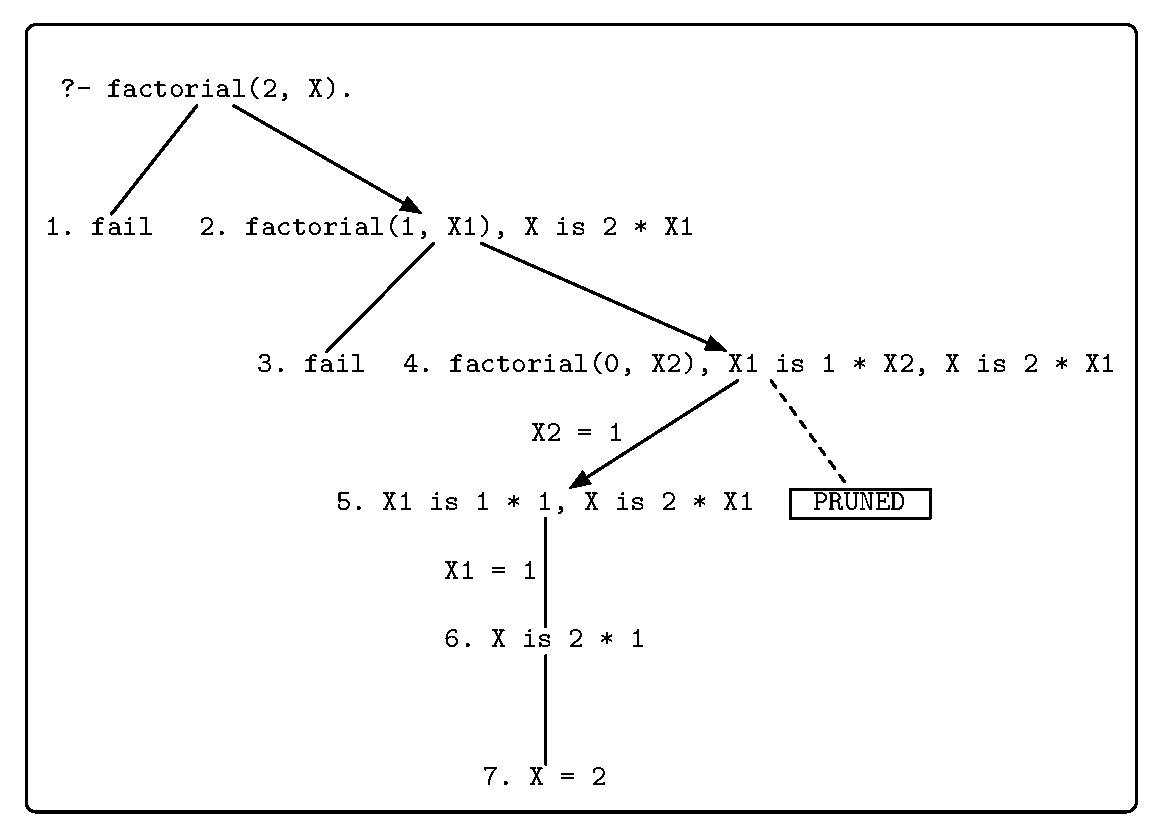
\includegraphics[scale=0.6]{factorial.pdf}
  \caption{Factorial search tree.}
  \label{fig:factorial_tree}
\end{figure}

The cut operator is not the only special instruction in Prolog, more built-in predicates are also available:

\begin{itemize}
  \item \textbf{Meta-logical predicates}: inquire the state of the computation and manipulate terms.
  \item \textbf{Extra-logical predicates}: manipulate the Prolog database, adding or removing clauses from
  the program being executed. Input/Output operators are another example of extra-logical predicates.
  \item \textbf{Other predicates}: predicates to perform arithmetic operations, to compare terms, to support debugging, etc.
\end{itemize}

These special operators make programming more practical and useful in real world applications.

\subsubsection{WAM}

The \textit{Warren Abstract Machine} (WAM) is a stack-based architecture
with various data areas, registers, and low level instructions that can be efficiently executed, manipulated and optimized.
A simplified layout is presented in Figure~\ref{fig:wam}.

\begin{samepage}
   
In terms of execution stacks, the WAM defines the following:

\begin{itemize}
  \item \textbf{PDL}: a push down list used by the unification process.
  \item \textbf{Trail}: stores the addresses of the variables that must be reset when backtracking.
  \item \textbf{Stack}: stores \textit{environment} and \textit{choice point} frames.
         Environments track the flow control in a program and consist of: the stack address of the
         previous environment; a pointer to the next instruction to execute upon return of the invoked
         clause; and a set of \textit{permanent variables} \footnote{A permanent variable is a variable
         which occurs in multiple body subgoals and must be preserved between calls.} as a sequence of cells.
         
         Choice points store open alternatives which are used to restore the state of the computation
         when backtracking. A pointer to the instruction for the next alternative is stored in case
         the current execution branch fails.
         A choice point is created when there are more than one alternative for a subgoal call.
         We pop the choice point from the stack when the last alternative clause is attempted. 
  \item \textbf{Heap}: array of data cells used to store variables and compound terms that cannot
         be stored in the stack.
  \item \textbf{Code Area}: contains the compiled instructions.
\end{itemize}

\end{samepage}

\begin{figure}[ht]
  \centering
    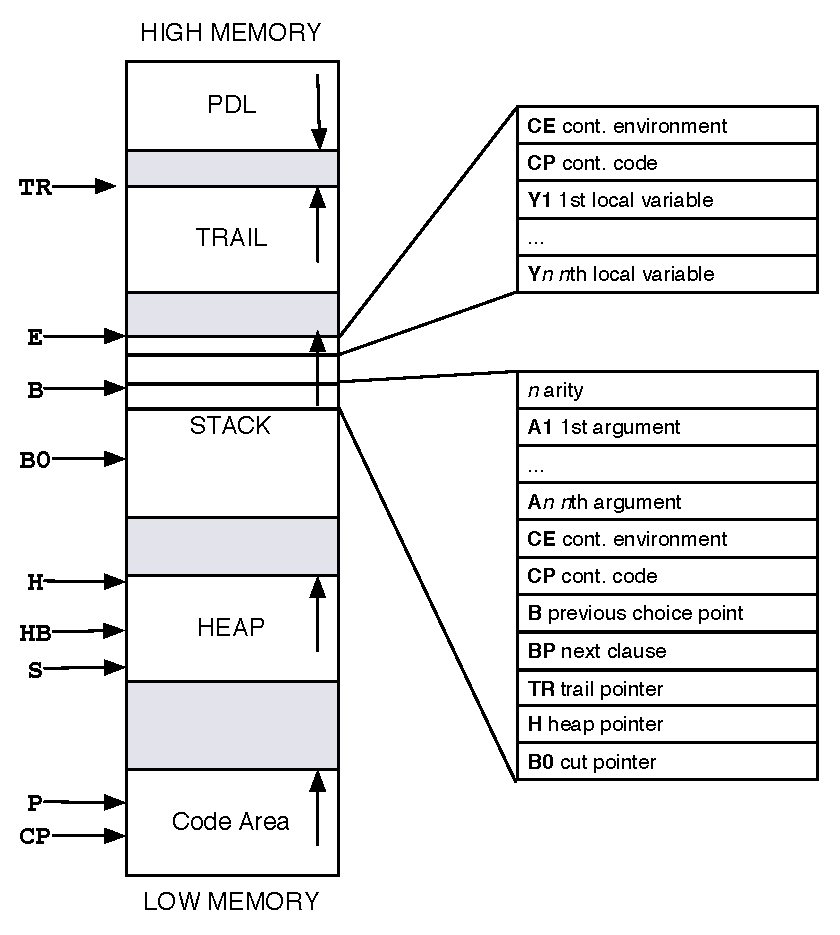
\includegraphics[scale=0.7]{wam.pdf}
  \caption{WAM memory layout, frames and registers.}
  \label{fig:wam}
\end{figure}

For the registers, WAM defines the following:

\begin{itemize}
  \item \textbf{P}: points to the current WAM instruction.
  \item \textbf{CP}: stores the value of \textbf{P} before the current invoked call and it is used to restore the execution point.
  \item \textbf{TR}: points to the top of the trail stack.
  \item \textbf{E}: points to the current active environment.
  \item \textbf{B}: the active choice point.
  \item \textbf{B0}: the choice point to return to upon backtracking over a cut.
  \item \textbf{H}: points to the top of the heap stack
  \item \textbf{HB}: marks the value of the register \textbf{H} at the time of the latest choice point. It is used to
  determine \textit{conditional} variable bindings that affect variables existing before the creation of the choice point.
  \item \textbf{S}: used during the unification of compound terms.
\end{itemize}

WAM instructions can be grouped into four main groups: choice point instructions to manipulate choice points; control
instructions to manage environments and control the execution flow; unification instructions that implement
specialized versions of the unification algorithm; and indexing instructions to efficiently determine which clauses
unify with a given subgoal call.

The WAM being a complex topic has complete books dedicated to explaining its intricacies.
An example is the \textit{Warren's Abstract Machine -- A Tutorial Reconstruction} written by H. A\"{\i}t-Kaci \cite{Aitkaci-91}. 

\section{Tabling}

Despite Prolog's declarativeness and expressiveness, the past few years have seen wide efforts at
solving shortcomings that arise when using SLD resolution.
One proposal that has gained popularity is \textit{tabling} or \textit{tabulation} \cite{Chen-96}.
In comparison to the traditional SLD resolution method, tabling can reduce the search space to cut redundant computations,
avoids looping and has better termination properties \cite{Tamaki-86}.

In a nutshell, tabling is a refinement of the SLD resolution that consists in storing intermediate answers for
subgoals so that they can be reused when a repeated subgoal appears in the resolution process.
The use of tabling enables the programmer to write more expressive, but still valid, logical programs.

One classical example that is used to demonstrate the advantages of using tabling is presented
in Figure~\ref{fig:prolog_path}. This program describes the predicate \texttt{path/2} that computes
reachability between two nodes on a directed graph. Connections are established as facts using the
\texttt{edge/2} predicate.

\begin{figure}[ht]
\begin{verbatim}
:- table path/2.

path(X,Z) :- edge(X,Y), path(Y,Z).
path(X,Z) :- edge(X,Z).

edge(a,b).
edge(b,a).
\end{verbatim}
\caption{The \texttt{path} program.}
\label{fig:prolog_path}
\end{figure}

If we tried to evaluate the query goal \texttt{path(X,Z)}, traditional Prolog would enter an infinite
loop (Figure~\ref{fig:infinite_loop}) because \texttt{edge/2} facts define a cyclic graph and the first
clause of \texttt{path/2} is right recursive, leading to a repeated call.

\begin{figure}[ht]
  \centering
    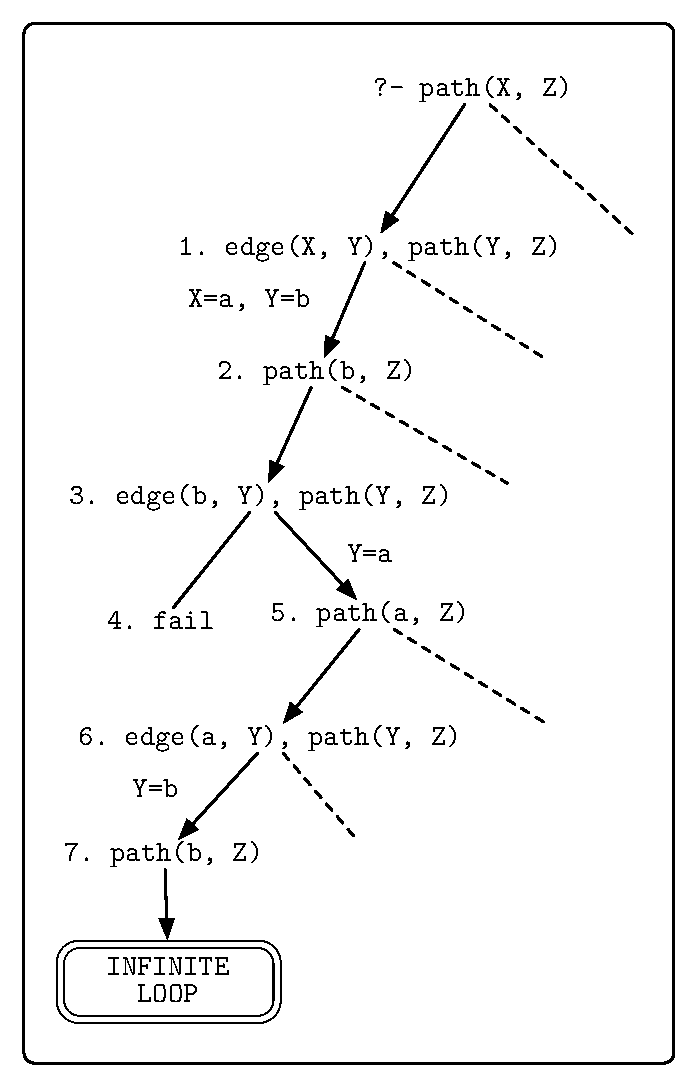
\includegraphics[scale=0.6]{infinite_loop.pdf}
  \caption{Infinite loop evaluating \texttt{path(X, Z)}.}
  \label{fig:infinite_loop}
\end{figure}

\subsection{Tabled Evaluation}

In this new method of evaluation, when a tabled subgoal is first called, a new entry is allocated on the \textit{table space}. Table
entries are used to store subgoal calls but they also store answers found during evaluation. Each time a tabled subgoal is called, we
know if it is a repeated call by inspecting the table space. Nodes in the search space can thus be classified as:
\textit{generator nodes}, if they are being called for the first time; \textit{consumer nodes} if they are repeated calls;
or \textit{interior nodes} if they are non-tabled subgoals. Generator nodes are matched against the predicate clauses as usual but
consumer nodes are not, instead they consume answers stored in the table space from the respective subgoal.

In Figure~\ref{fig:tabling_path} we depict the tabled evaluation of the query goal \texttt{path(X,Z)}.
Generator nodes are represented by rectangles with double lines and consumer nodes by simple rectangles.
Note that we need to declare \texttt{path/2} as tabled using the \texttt{table} directive.

Tabled evaluation starts by inserting a new entry in the table space and by allocating a generator
node to represent \texttt{path(X,Z)} (step 1). Like SLD resolution, \texttt{path(X,Z)} is then resolved
against the first \texttt{path/2} clause (step 2). The goal \texttt{edge(X,Y)} is not tabled and is
resolved as usual. We use the first \texttt{edge/2} clause with \texttt{\{X~=~a,~Y~=~b\}} and these values
are carried to \texttt{path(b,Z)} (step 3). This goal is not yet in the table space, hence we add a new entry for it.

Goal \texttt{path(b,Z)} is then resolved against the first clause of \texttt{path/2} (step 4).
Ñext, \texttt{edge(b,Y)} fails against the first clause but succeeds with \texttt{\{Y~=~a\}} for
the second clause. A new tabled subgoal \texttt{path(a,Z)} is registered in the tabled space (step 6)
and resolved against the first clause of \texttt{path/2} (step 7). This time the \texttt{edge/2}
subgoal matches with the first clause with \texttt{\{Y~=~b\}}. This originates a repeated tabled subgoal
call to \texttt{path(b,Z)} and the first consumer node is allocated (step 8). As we have no answers for \texttt{path(b,Z)}
in the table space, the current evaluation point is \textit{suspended}. Later on, this node can be resumed to
consume new answers.

Next, we backtrack to node 7 and try the second \texttt{edge/2} clause, but resolution fails (step 9). We backtrack again, this time to
node 6 to try the second clause of \texttt{path/2} (step 10). Here \texttt{edge(a, Z)} is resolved against the
first clause of \texttt{edge/2} and the answer \texttt{\{Z~=~b\}} is found for the subgoal \texttt{path(a,Z)} (step 11).
This answer is stored in the table space and forward execution is made, propagating the binding \texttt{\{Z~=~b\}} to
\texttt{path(b,Z)}, and a first answer to this subgoal is also found and stored in the table space (step 12).
We continue forward execution and the binding is once again propagated, this time to node 3 finding an answer to
\texttt{path(X,Z)} and to the query subgoal, \texttt{\{X~=~a,~Z~=~b\}} (step 13).

\begin{figure}[ht]
  \centering
    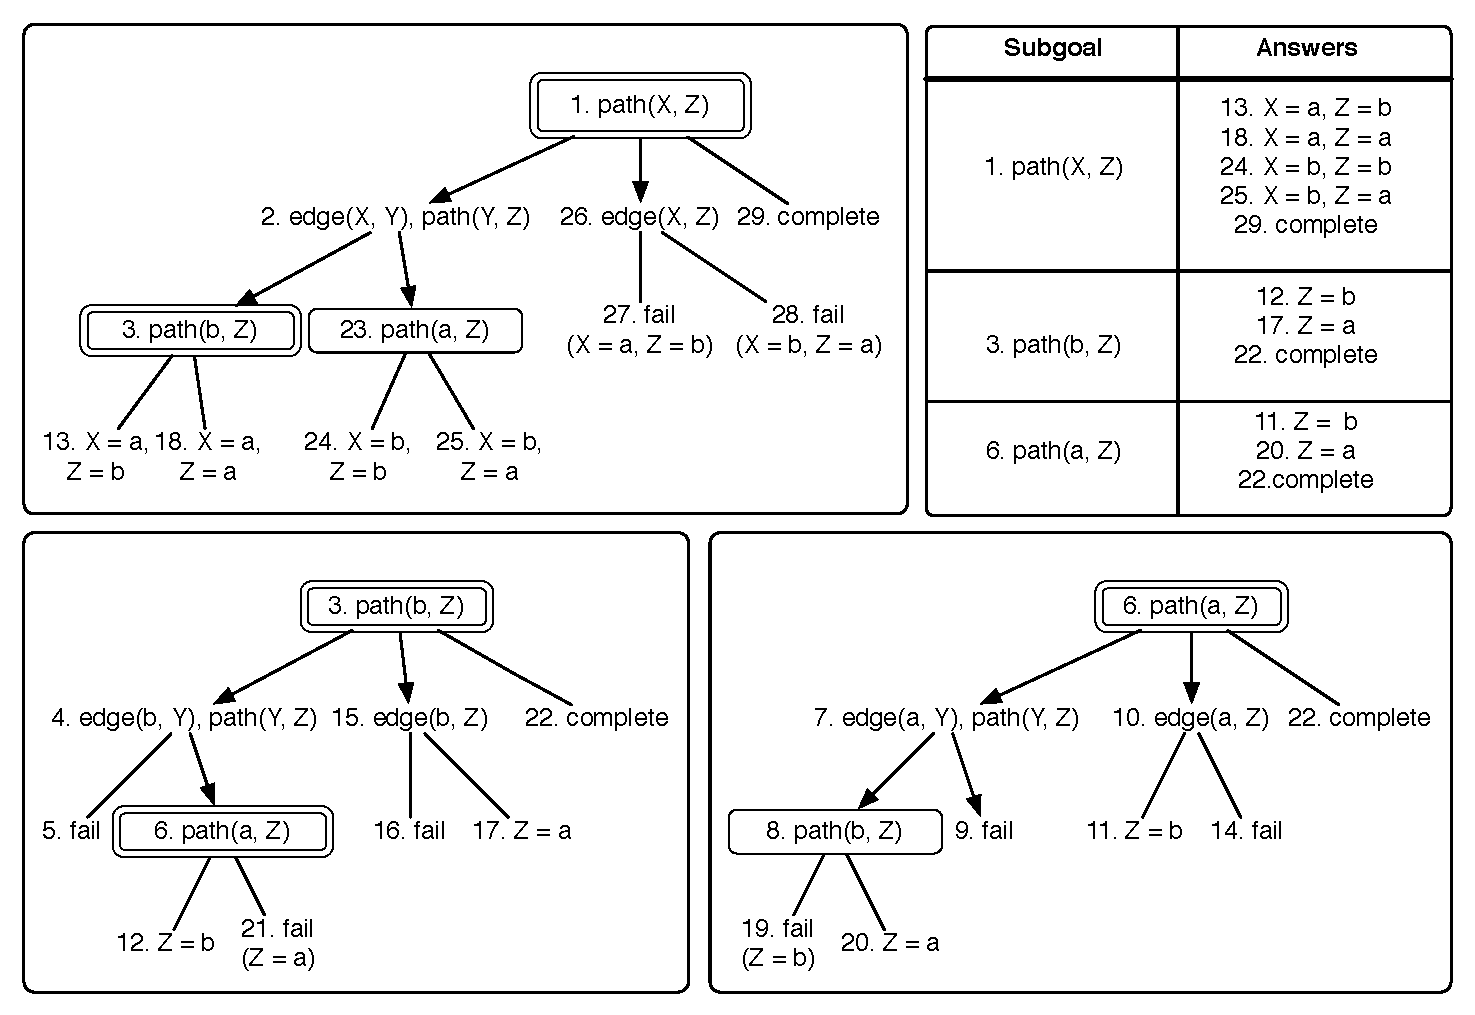
\includegraphics[scale=0.6]{tabling_path.pdf}
  \caption{Tabled evaluation of \texttt{path(X,Z)}.}
  \label{fig:tabling_path}
\end{figure}

If the user asks for more answers, the computation returns to node 10 to try the second clause of
\texttt{edge/2}, but it fails (step 14). The process backtracks to node 6 but at this node there
are no more clauses left to try. Moreover, we can not complete the subgoal \texttt{path(a,Z)} because
it depends on a older subgoal (node 3 is the generator node for the consumer node 8 under it), thus we backtrack to node 3.

At node 3, the second clause of \texttt{path/2} is tried (step 15) and the first clause of
\texttt{edge/2} fails (step 16), but the second succeeds with a new answer for \texttt{path(b,Z)},
\texttt{\{Z~=~a\}} (step 17). Again, we propagate variable bindings in step 18, generating a new
answer to subgoal \texttt{path(X,Z)}, \texttt{\{X~=~a,~Z~=~a\}}.

We go back to node 3, where no more clauses are available, but now completion can be safely
attempted because all consumers in lower branches do not depend on any generator node older
than node 3. Node 3 is called, by definition, a \textit{leader node} and the branch of nodes
below it form a \textit{Strongly Connected Component} (SCC) \cite{Tarjan-72}.

However, by inspecting the execution tree, we can see that node 8 has two unconsumed answers.
We thus resume the computation at node 8 to consume the answer \texttt{\{Z~=~b\}} and forward it to subgoal
\texttt{path(a,Z)} at node 6 (step 19). Here, we note that it is a repeated answer
to this subgoal by checking the table space, and thus we fail (step 19).
Failing repeated answers is crucial to avoid unnecessary computations and sometimes looping.

Then, we fetch the next available answer, \texttt{\{Z~=~a\}}, that is propagated
to node 6, generating a new answer to \texttt{path(a,Z)} (step 20). This binding
is once again propagated, now for node 3 but it is a repeated answer, and thus
the computation fails (step 21). With no more unconsumed answers, we
return back to node 3 to re-attempt completion. This time, no consumers have
unconsumed answers and we can safely complete all the subgoals in the current SCC
(step 22). Subgoals \texttt{path(b,Z)} (node 3) and \texttt{path(a,Z)} (node 6)
are marked as \textbf{complete} in the table space and no new answers are accepted.

Next, we backtrack to node 2 to try the second \texttt{edge/2} clause. A new consumer node is allocated (step 23) and answers can be
promptly consumed from the table space as the subgoal \texttt{path(a,Z)} is already completed.
The retrieved answers in step 23 are propagated to node 1 and new answers are generated (steps 24 and 25).

We backtrack to node 1 to try the second \texttt{path/2} clause (step 26). Resolution succeeds for both
\texttt{edge/2} clauses but as the newly found answers
are repeated we fail for both cases (steps 27 and 28). The process backtracks again to node 1 and with no more clauses to try,
we attempt completion. As there are no consumer nodes, completion is done (step 29) and computation terminates successfully.

From the described example we can summarize four main operations needed to support tabled evaluation:

\begin{itemize}
  \item The \textit{tabled subgoal call} operation represents a call to a tabled subgoal.
  If the subgoal is already in the table space, it creates a new consumer node to consume answers.
  If it is a new subgoal call it creates a new generator node and adds a new entry to the table space.
  Each new entry is initialized with an empty set $S$ that will contain the answers for the subgoal. 
  
  \item The \textit{new answer} operation adds a new answer $s$ to the table space. If the answer is repeated the operation fails,
  otherwise a new answer set $S'$ for the subgoal is generated: $S' \equiv S \cup {s}$.
  
  \item The \textit{answer resolution} operation checks wether new answers from the table space are available for consumption.
  When no new answers are available, the consumer node is \textit{suspended} and execution proceeds using a specific strategy.
  Given the last consumed answer, we determine the unconsumed answer
  set $R$ ($R \subseteq S$) and fetch the element $r \in R$, which is the first element from the set $R$. The last consumed answer
  can be seen as a \textit{continuation} that is stored in each consumer node and is used to determine the next available answer.
  
  \item The \textit{completion} operation determines if a tabled subgoal is \textit{completely evaluated}.
  Only leader nodes can complete themselves and younger generator nodes.
  Once a subgoal is completed the set of answers $S$ is closed and no more answers are accepted; future subgoal calls
  can use the set $S$ without the need to suspend.
\end{itemize}

\subsection{Tabling Instructions}

Tabling engines extend the WAM instruction set with \textit{tabling instructions} to support the four
main tabling operations. Usually, each tabled predicate is compiled by using
variants of the following instructions:
\texttt{table\_try}, \texttt{table\_retry} and \texttt{table\_trust}. These instructions
are very similar to \texttt{try\_me}, \texttt{retry\_me} and
\texttt{trust\_me}, which the WAM natively implements. 

For tabled predicates with multiple clauses, \texttt{table\_try} is used on the first clause,
\texttt{table\_retry} for the middle clauses and \texttt{table\_trust} for the last clause.
Predicates with a single clause use a special instruction: \texttt{table\_try\_single}.

\begin{figure}[ht]
\begin{Verbatim}
path/2_1:
  table_try_me path/2_2
  % WAM code for path(X,Z) :- edge(X,Y), path(Y,Z).
  new_answer
path/2_2:
  table_trust_me
  % WAM code for path(X,Z) :- edge(X,Z).
  new_answer
\end{Verbatim}
\caption{Compiled code for the tabled predicate \texttt{path/2}.}
\label{fig:compiled_tabled_path}
\end{figure}

The \texttt{table\_try} instruction implements the tabled subgoal call operation. If the subgoal is called
for the first time, the data structures associated with this subgoal and a new generator node are created.
Execution then proceeds by executing each predicate clause. This is performed by the \texttt{table\_retry}
instruction, which alters the next instruction of the generator choice point to the next clause of the predicate.
On the other hand, if the subgoal is repeated, a consumer choice point is allocated and set to execute the
\texttt{answer\_resolution} instruction, which consumes answers and implements the answer resolution operation.

The instruction \texttt{table\_trust} is executed by generator nodes and sets the next
instruction to execute upon backtracking to
\texttt{completion}, which runs the completion operation.

Finally, at the end of each clause, the instruction \texttt{new\_answer} is appended to implement
the new answer operation. This instruction has access to the arguments of a tabled subgoal call,
thus by dereferencing them it obtains the corresponding answer, which can be added into the table space.    

\subsection{Scheduling Strategies}

During evaluation of the previous example it is very clear that at several points we can choose between
different \textit{scheduling} strategies: continue forward execution, backtrack to interior nodes,
return answers to consumer nodes, or perform completion. Depending on how and when the return of answers
is scheduled, different strategies and searches can be formulated. It is also well known that using
different strategies can lead to tremendous effect on performance as some predicates are better suited to specific strategies. 
The most popular scheduling strategies are \textit{batched scheduling} and \textit{local scheduling} \cite{Freire-96}.

Batched scheduling reduces the need to suspend and move around the search tree by batching the return of answers.
When the engine generates answers, while evaluating a particular goal, the answers are added to the table and
the subgoal continues its normal evaluation until it resolves all available program clauses. Only then the answers
are consumed by consumer nodes \cite{Freire-96}. In some cases, this results in creating dependencies to older
subgoals, therefore enlarging the current SCC and delaying completion to older generator nodes. When backtracking,
three situations may arise:

\begin{itemize}
  \item if backtracking to a generator or interior node, try the next available clause.
  \item if backtracking to a consumer node, consume new answers.
  \item if no more clauses are left to try or no more unconsumed answers are available, two new situations may arise:
    \begin{itemize}
      \item if the node is a leader node, attempt completion.
      \item if not, backtrack to a previous branch.
    \end{itemize}
\end{itemize}

Note that batched scheduling was the strategy used in the evaluation of the example in Figure~\ref{fig:tabling_path}.

For some problems, local scheduling is better suited because it tries to evaluate a single exact SCC at a time, preserving the dynamic
SCC ordering during the evaluation. In other words, in a local evaluation, answers are returned to consuming nodes outside of an SCC only after that
SCC is completely evaluated \cite{Freire-96}.
It differs from batched scheduling in that once the answers are found, they are added to the table space, but execution
\textit{fails}. Because this strategy tries to complete sooner rather than later, we can expect less dependencies between subgoals.

\subsection{Variant Tabling} \label{sec:variant_tabling}

When the subgoal \texttt{path(X,Z)} is called, a check for the presence of this subgoal in the table space is done first.
In the example in Figure~\ref{fig:tabling_path}, this was done by checking wether a \textit{variant} of the new goal already
exists in the table. We say that two terms $t_1$ and $t_2$ are variants of each other if they are identical up to renaming of their
variables.

For example, \texttt{path(X,Z)} is variant of the subgoal \texttt{path(X,Y)}, as they represent the same subgoal if we try
to rename their variables to a standardized format. One format was proposed by Bachmair \textit{et al} \cite{Bachmair-93}. Formally,
we have a set $V$ of variables present in a term and a function $renameVar$, such that the first term variable $v0 \in V$
results in $renameVar(v0) = VAR0$ and the following distinct variables are named incrementally ($VAR1, VAR2, ...$).
Using this mechanism, \texttt{path(X,Z)} and \texttt{path(X,Y)} both result in \texttt{path(VAR0,VAR1)}. The resulting
standardized subgoal is then checked against the table space to verify if it is a repeated subgoal call.

The variant approach is widely used in tabling systems, but other approaches do exist. One approach named
\textit{call by subsumption} works by checking wether the new goal is subsumed by another goal in the table space.
In other words, we verify if there is a more general subgoal than the one being called. For example
\texttt{path(b,Z)} is subsumed by the subgoal \texttt{path(X,Z)}.

In this approach, instead of creating a new generator node at step 3, we create a consumer node that would consume
answers stored in the subgoal \texttt{path(X,Z)}. For correct results, it should be clear that the answers used
from the table space must unify with \texttt{path(b,Z)}. Like variant tabling, those new consumer nodes do not expand
by using the program clauses, hence the search tree for this new method will be greatly reduced.

Variant and subsumption-based tabling define the \emph{call similarity} property of the tabling engine. In
a nutshell, when a subgoal $A$ is declared to be \emph{similar} to subgoal $B$, we say that $A$ consumes from
$B$ ($A$ is a consumer) and $B$ generates its own answers.

  \subsection{Yap and XSB}
  
  Yap \cite{system-yap} and XSB \cite{system-xsb} are two well known Prolog systems that implement tabling.
  
  The YAP Prolog system is a high-performance Prolog compiler developed at the University of Porto.
  It is one of the fastest available Prolog systems and implements a wide range of functionalities: 
  stream I/O, sockets, modules, exceptions, debugging, a C-interface, dynamic code, internal database,
  DCGs, saved states, co-routining, arrays, threads and tabling.
  It is based on the WAM and follows the Edinburgh tradition. Most of the ISO-Prolog standard is implemented.
  
  Tabling in Yap is implemented through the YapTab sub-system \cite{Rocha-05a}, a suspension based tabling engine supporting evaluation of
  definite programs. YapTab follows the seminal SLG-WAM (Linear resolution with Selection function for General logic programs in WAM)
  design from XSB Prolog \cite{Sagonas-96, Sagonas-98},
  but it innovates by proposing a new fix-point check algorithm, and by considering that the control of fix-point detection should be
  performed at the level of the data structures corresponding to suspended sub-computations. YapTab was originally designed to achieve
  good results in sequential tabling, but could be extended with the OPTYap engine, for parallel execution \cite{Rocha-05a}.
  Other innovations in YapTab include: support for a dynamic combination of batched and local scheduling \cite{Rocha-05c}
  and efficient handling of \textit{incomplete tables} \cite{Rocha-06b}. Incomplete tables are created when the current computation is pruned from the execution stacks, keeping the pruned subgoals from retrieving
  the complete answer set. Currently, only call by variant checking is supported.
  
  XSB is a research-oriented logic programming system for Unix and Windows based systems. In addition to providing all
  the functionality of the Prolog language, XSB contains several features not usually found in logic programming systems,
  namely, evaluation according to the Well-Founded Semantics (tabling with negation) \cite{Gelder-91} through the use of
  a delaying-based tabling engine, the SLG-WAM.
  Other features of XSB include: a fully threaded engine, constraint handling for tabled programs on a engine level, a variety of indexing
  techniques, interfaces to other languages, various compiler directives like \texttt{auto\_table}, which does static
  analysis to decide which predicates to table, etc. \cite{system-xsb}.
  
  SLG-WAM supports both tabling by variant checking and by subsumption checking.
  Tabling by call-subsumption was initially implemented by a technique called
  \textit{Dynamic Threaded Sequential Automata} \cite{Rao-96} and is currently
  implemented using \textit{Time Stamped Tries} \cite{Johnson-99}.

  In terms of design, both YapTab and SLG-WAM introduce the following extensions to the traditional WAM machine:
  the table space; a new set of registers, the \textit{freeze registers}, one per stack (local stack, heap and trail);
  an extension of the standard trail,
  called the \textit{forward trail}; and the tabling operations: \textit{tabled subgoal call},
  \textit{new answer}, \textit{answer resolution}, and \textit{completion}.

  The set of freeze registers says where stacks are frozen and protect the space belonging to suspended
  computations until the completion of the appropriate SCC takes place. They need to be adjusted
  in two different situations: when a computation suspends, increasing the portion of frozen stacks; and when a completion takes place,
  releasing part of space previously frozen.

  The forward trail is used to restore all the variable bindings to their state at the time the computation was suspended.
  Thus, the WAM trail is extended with parent trail entry pointers to create this new trail.
  Also, a new register is created, the \textbf{TR\_FZ} trail freeze register.

  The differences between SLG-WAM and YapTab reside in the data structures and algorithms used to control the process of leader detection
  and the scheduling of unconsumed answers. These differences are described next in more detail.
  
  \subsubsection{SLG-WAM}

  The SLG-WAM considers that evaluation control should be done at the level of the data structures
  corresponding to first calls to tabled subgoals, and does so by associating \textit{completion frames}
  to generator nodes \cite{Sagonas-98}.

  The \textit{completion stack} maintains, for each subgoal $S$, a representation of the deepest subgoal
  $S_{dep}$ upon which $S$ or any subgoal on top of $S$ may depend.

  When $S$ and all subgoals on top of $S$ have exhausted all program and answer clause resolution,
  $S$ is checked for completion. If $S$ depends on no subgoals deeper than itself, $S$ and
  all subgoals on top of $S$ are completely evaluated. Otherwise, if $S_{dep}$ is deeper in the completion
  stack than $S$, $S$ may depend upon subgoals that appear below it in the completion stack, and cannot be completed \cite{Sagonas-98}.

  A one-to-one correspondence exist between completion stack frames and generator nodes, as the completion stack frame
  is pushed onto the stack when a new tabled subgoal is called. A completion frame is popped off when a subgoal is
  completed. Also, each subgoal frame contains a pointer to completion frame.

  Consumer and generator choice points are extended to support the suspend and resume mechanism.
  The generator choice contains the following extra data: an explicit pointer of the failure continuation to take
  upon backtracking out of the choice point; a cell that records the value of a new global register,
  called the \textbf{RS} (\textit{root subgoal register}) register,
  which points to the root subgoal of the node currently under execution;
  a pointer to the subgoal frame; a set of freeze registers, so that the stored values can be restored later on;
  and an area called the \textit{substitution factor}, the set of free variables which exist in the terms in the argument registers.

  The consumer choice point is extended with: a copy of the \textbf{RS} register; a pointer of the failure continuation to take
  upon backtracking; a substitution factor; the last consumed answer continuation; and a pointer to chain
  together all consumer choice points of the same subgoal. 

  \subsubsection{YapTab}

  In YapTab, it is considered that the control of leader detection and scheduling of unconsumed answers should be
  performed through the data structures corresponding to repeated calls to tabled subgoals, and it associates a new
  data structure, the \textit{dependency frame}, to consumer nodes \cite{Rocha-00a}. Each consumer choice point thus
  contains a field that points to the respective dependency frame.

  Dependency frames are used to check for completion points and to move across the consumer nodes with unconsumed answers,
  thus they are linked together, forming the \textit{dependency space}.

  Generator choice points are WAM choice points extended with the substitution factor area, a pointer
  to the subgoal frame and, a pointer to a dependency frame. This pointer
  is only used when local scheduling is employed. A generator node for local scheduling only exports its answers to the calling
  environment when all clauses for the subgoal have been exhausted, hence it must act like a consumer.

  In SLG-WAM, if we want to release space previously frozen and restore the freeze registers, we use the
  stack values stored in the generator choice point to perform completion. In YapTab, as the freeze registers
  are not saved there, we use the top stack values kept in the youngest consumer choice point younger than the current completion point.

  YapTab reduces the size of consumer choice points by using dependency frames. Each frame contains the
  following fields: \textbf{last\_answer} field that stores the last answer consumed by the choice point;
  the \textbf{cons\_cp} field that points to the consumer choice point; the \textbf{leader} field which
  points to the leader node at creation time; and the \textbf{back\_leader} field that changes during
  evaluation, pointing to the leader node where we performed the last unsuccessful completion operation.
  A new global register, called \textbf{TOP\_DF}, always points to the youngest dependency frame.

\section{Chapter Summary}

In this chapter we introduced logic programming and Prolog. We discussed the shortcomings of the
SLD resolution and then we presented tabling, which is a technique that solves these problems.

Next, we discussed how tabled programs are evaluated, by introducing the concepts of generator,
consumer, scheduling strategies, such as batched scheduling and local scheduling, and
the call similarity property in variant and subsumption-based tabling engines.
We also discussed two of the most widely known Prolog systems that implement tabling, Yap and XSB Prolog.

In the next chapter we will throughly discuss and analyze how the table space is organized to efficiently
implement variant-based tabling and then subsumption-based tabling.


\newpage
\thispagestyle{plain}
\mbox{}

\chapter{Table Space Organization}

In this chapter, the table space organization for both variant and subsumption tabling
engines are described. First, the variant table space for both SLG-WAM and YapTab is
explained. Because they share a lot of similarities, the description covers the common
ground between the two systems. Next, we explore two well-known mechanisms that modify
the previous table space for call by subsumption. Those two mechanisms have already been
implemented in XSB Prolog \cite{Rao-96, Johnson-99}.

\section{Table Space} \label{sec:table_space}

Implementing a tabling engine on a Prolog system involves the design of compact and time efficient data structures
to organize the table space. The table space is heavily used throughout the evaluation process in various operations:

\begin{itemize}
  \item to lookup if a subgoal is in the table, and if not insert it;
  \item to verify whether a newly found answer is already in the table, and if not insert it;
  \item to retrieve answers for consumer nodes.
\end{itemize}

\subsection{Tries}

Clearly, the success of tabling is highly dependent on the data structures used.
Both the YapTab \cite{Rocha-00a} and SLG-WAM \cite{RamakrishnanIV-95} engines use a trie-based approach.

Tries were initially proposed to index dictionaries \cite{Fredkin-62} and have since been generalized to index recursive data structures
such as terms. The essential idea underlying a trie is to partition a set $T$ of terms based upon their structure,
in such a way that common term prefixes are represented only once.

A trie is a tree-structured automaton with the root as the start state and each leaf state associated with a term in $T$.
Each state specifies the position to be inspected in the input term on reaching that state.
The outgoing transitions specify the function symbols expected at that position.
A transition is taken if the current symbol in the input term matches the symbol of the transition.
If we recursively reach a leaf state we say that the input term \textit{matches} the term represented by the leaf state.
A complete path, from the root to a leaf, corresponds to a pre-order traversal of the matching term.
If no transition can be taken, the lookup operation fails. On the other hand, for an insert operation
we add a new outgoing transition for the current input symbol and a new node, which is linked to this transition.
To complete the insert operation, we consume the rest of the input term, until a leaf node is created that represents
the newly inserted term.

Given the nature of tries, the following conclusions can be made:

\begin{itemize}
  \item the lookup/insert operation can be done in a single pass through a term. If the lookup fails, it is possible
  to complete an insert operation using the last lookup state;
  \item the efficiency and memory consumption of a
  particular trie depends on the percentage of terms that have common prefixes.
\end{itemize}

When creating transitions for variables, we use the format outlined by Bachmair \textit{et al.} \cite{Bachmair-93},
that was described in Section \ref{sec:variant_tabling}.

Figure~\ref{fig:tries_use} shows a trie with three terms. First, in (a) the trie is represented by a \textit{root node} and has
no terms. Next, in (b) the term \texttt{t(X,a)} is inserted and three nodes are created that represent each part of the term.
In (c) a new term, \texttt{u(X,b,Y)} is inserted. This new term differs from the first one and a new distinct branch is created.
Finally, in (d), the term \texttt{t(Y,1)} is inserted and only a new node needs to be created as this term shares
two prefix nodes with \texttt{t(X,a)}.

\begin{figure}[ht]
  \centering
    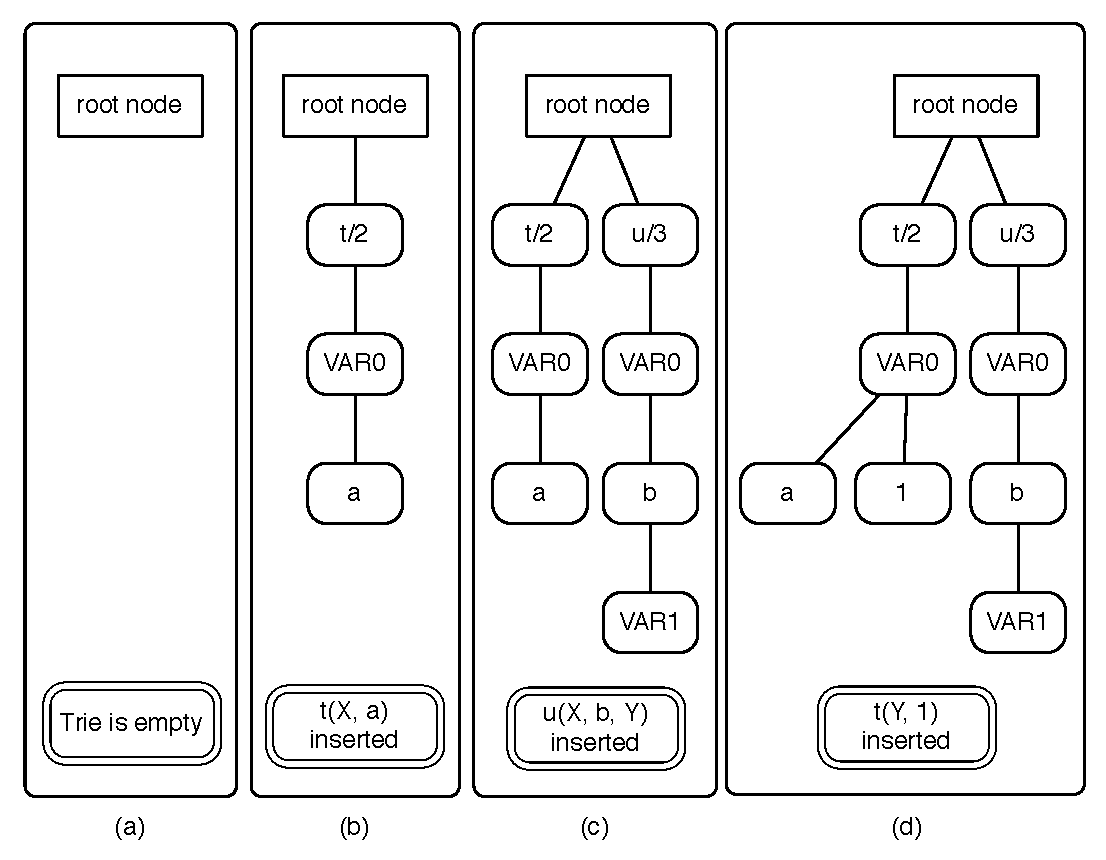
\includegraphics[scale=0.6]{tries.pdf}
  \caption{Using tries to represent terms.}
  \label{fig:tries_use}
\end{figure}

Yap and XSB use two levels of tries to implement the table space (see Figure~\ref{fig:table_space_tries}):

\begin{itemize}
  \item The first level, the \emph{subgoal trie}, stores subgoal calls for each predicate;
  \item The second level, the \emph{answer trie}, stores answers for a specific subgoal.
\end{itemize}

\begin{figure}[ht]
   \centering
     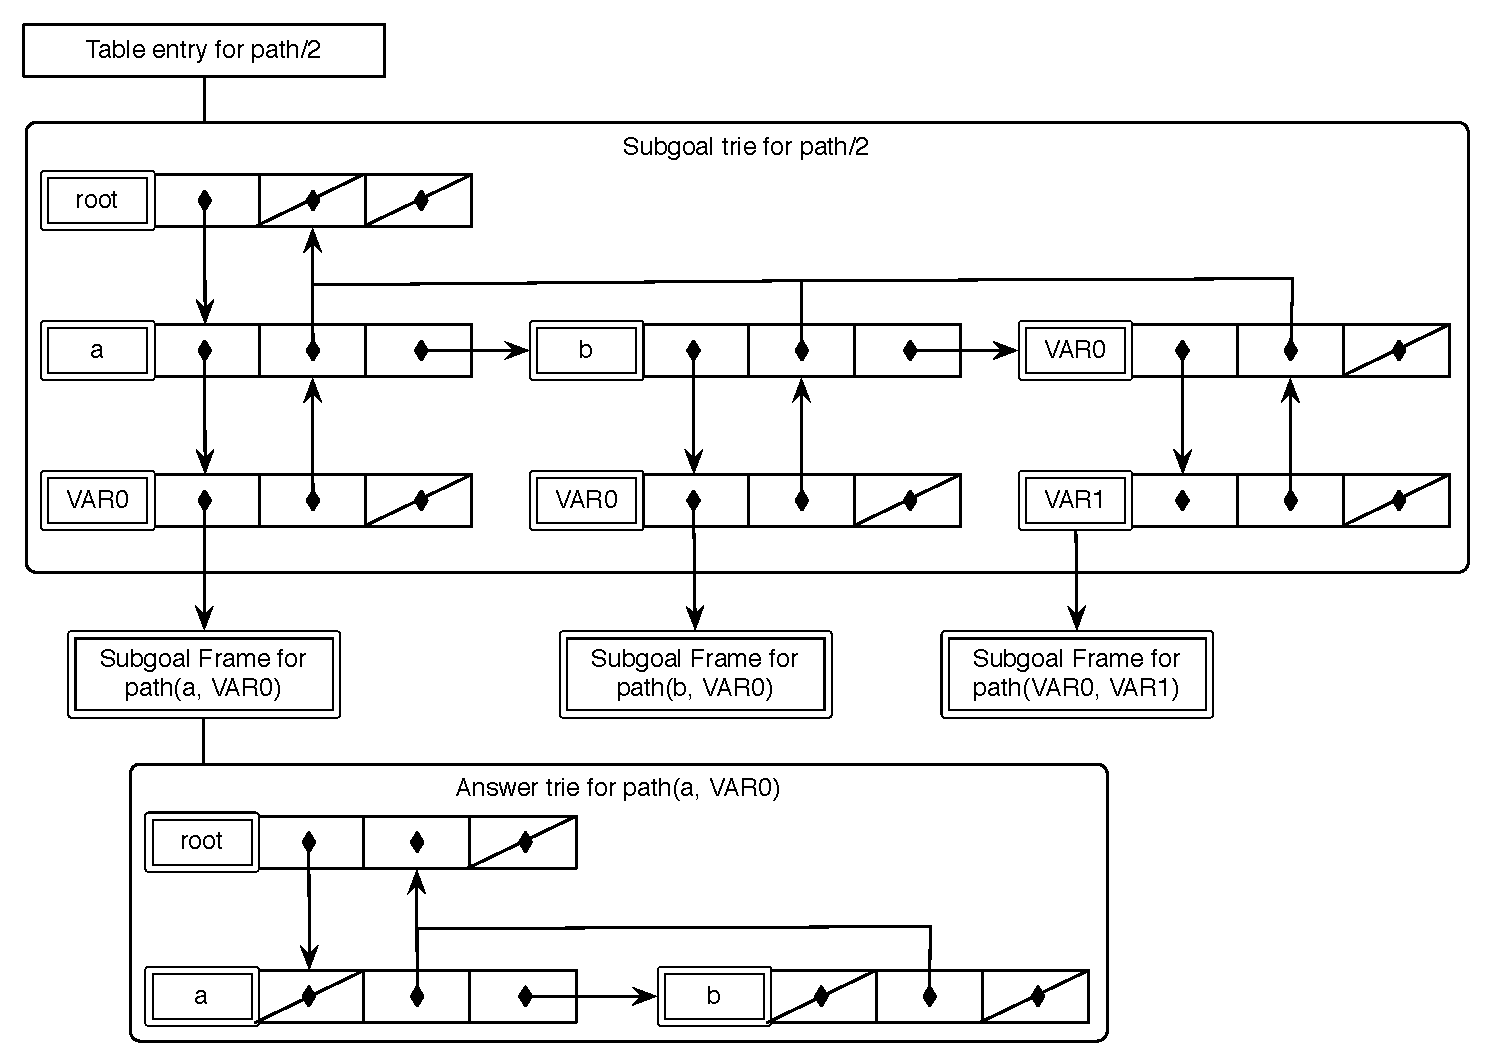
\includegraphics[scale=0.6]{two_level_tries.pdf}
   \caption{Organizing the table space with tries for variant tabling.}
   \label{fig:table_space_tries}
 \end{figure}

For both levels, each trie node usually contains four fields. The first field represents the \texttt{symbol}
(or \texttt{atom}) of the transition. The second points to the first descendant transition (called the \texttt{child} node)
and the third stores a pointer to the \texttt{parent} node.
The fourth field points to a \texttt{sibling} node, if any.

When the chain of sibling nodes gets too big, an hashing scheme is dynamically employed to provide direct
access to nodes, optimizing the search of transitions.

Each tabled predicate contains a \textit{table entry} that points to a \textit{subgoal trie}.
Each different call to a tabled predicate corresponds to a unique path through the subgoal trie.
Notice that for the subgoal trie only the subgoal arguments are stored.
The leaf points to a data structure called \textit{subgoal frame}. The subgoal frame stores
information about the subgoal, namely an entry point to its \textit{answer trie}.

The answer trie stores answers to the subgoal. When inserting answers, only substitutions
for the variables in the call are stored. This optimization is called \textit{substitution factoring} \cite{RamakrishnanIV-95}.

Figure~\ref{fig:table_space_tries} shows the table space organization after evaluating the query goal
\texttt{path(X,Z)} for the example in Figure~\ref{fig:tabling_path}.
The figure shows how the subgoals \texttt{path(X,Z)}, \texttt{path(b,Z)} and \texttt{path(a,Z)} are
stored in the \texttt{path/2} subgoal trie and how the answer trie for \texttt{path(a,Z)} is represented.
Notice that by using substitution factoring for the answer trie, only the substitutions
\texttt{\{VAR0~=~b\}} and \texttt{\{VAR0~=~a\}} need to be stored.

\subsection{Subgoal Frames}

A subgoal frame contains general information about the state of a tabled subgoal. To access answers, this
frame contains a pointer to the root of the answer trie. A chain of answers used by consumers is also kept
in the form of head and tail pointers. In XSB Prolog, a \textit{answer return list} is built and the consumer has
a pointer to the node of the list representing the last consumed answer. In Yap, answers are chained using
the \texttt{child} pointer of the leaf answer nodes and consumers only keep the last consumed answer leaf.
The last consumed answer pointer is an \textit{answer continuation}. When a consumer needs to verify
or consume the next available answer, it uses the continuation to retrieve the next answer, following the
chain of answers. To load an answer, the trie nodes are traversed in bottom-up order and the answer is
reconstructed.

To simplify memory management, both systems link subgoal frames by storing
\texttt{next} and \texttt{previous} pointers in each subgoal frame, forming a double linked list.
The evaluation state of the subgoal is also stored. For example, YapTab has the following states:
\textit{ready}, \textit{evaluating}, \textit{complete} and \textit{incomplete}.

\section{Tabling by Call Subsumption} \label{sec:subsumption}

Although variant based tabling has proven to be greatly beneficial in solving some shortcomings of the SLD resolution,
other approaches are possible. Tabling by call subsumption aims to reuse answer computations by sharing answers from
\textit{more general} subgoals \cite{Johnson-99}.

When a subgoal is first called, a variant engine will lookup in the table space for a variant subgoal, i.e.,
one that is identical by renaming the variables. If such a subgoal already exists on the subgoal trie, a new
consumer is created and the available answers from the variant subgoal are pushed for consumption.

Although a variant check is a light-weight operation computationally,
tabling engines using such checks can end up computing answers through program clause resolution, which takes time and space,
when they could retrieve answers from a subgoal that \textit{subsumes} the new call. By other words, a more specific subgoal
could consume answers from a general subgoal, which contains the set of relevant answers for the specific subgoal in
its answer set.

Formally, if two subgoals $G$ and $G'$ exist, such that $S$ and $S'$ are the respective answer sets and
$G'$ subsumes $G$, then we can conclude that $S \subseteq S'$.

The effects of using subsumptive checks are greater reuse of computed answers and reduced program clause resolution, yielding
superior time performance and memory usage. In terms of memory usage, improvements can be made since fewer calls and their
associated answer sets need to be preserved \cite{Johnson-99}. However, implementing call subsumption poses various challenges:

\begin{enumerate}[(a)]
\item How to efficiently check for subsuming subgoals in the subgoal trie;
\item How to design new mechanisms to represent answers supporting fast retrieval of subsets that are only related to a subsumed call;
\item How to support incremental retrieving of the answer subset. Note that, during evaluation, it may be not possible for
the subsuming call to contain all answers, as the process of generating answers is incremental.
\end{enumerate}

For illustration purposes, in Figure~\ref{fig:tabling_path_sub}, we describe the evaluation of \texttt{path(X,Z)}
using the program presented in Figure~\ref{fig:prolog_path}
and compare it against the variant approach in Figure~\ref{fig:tabling_path}.

\begin{figure}[ht]
\centering
  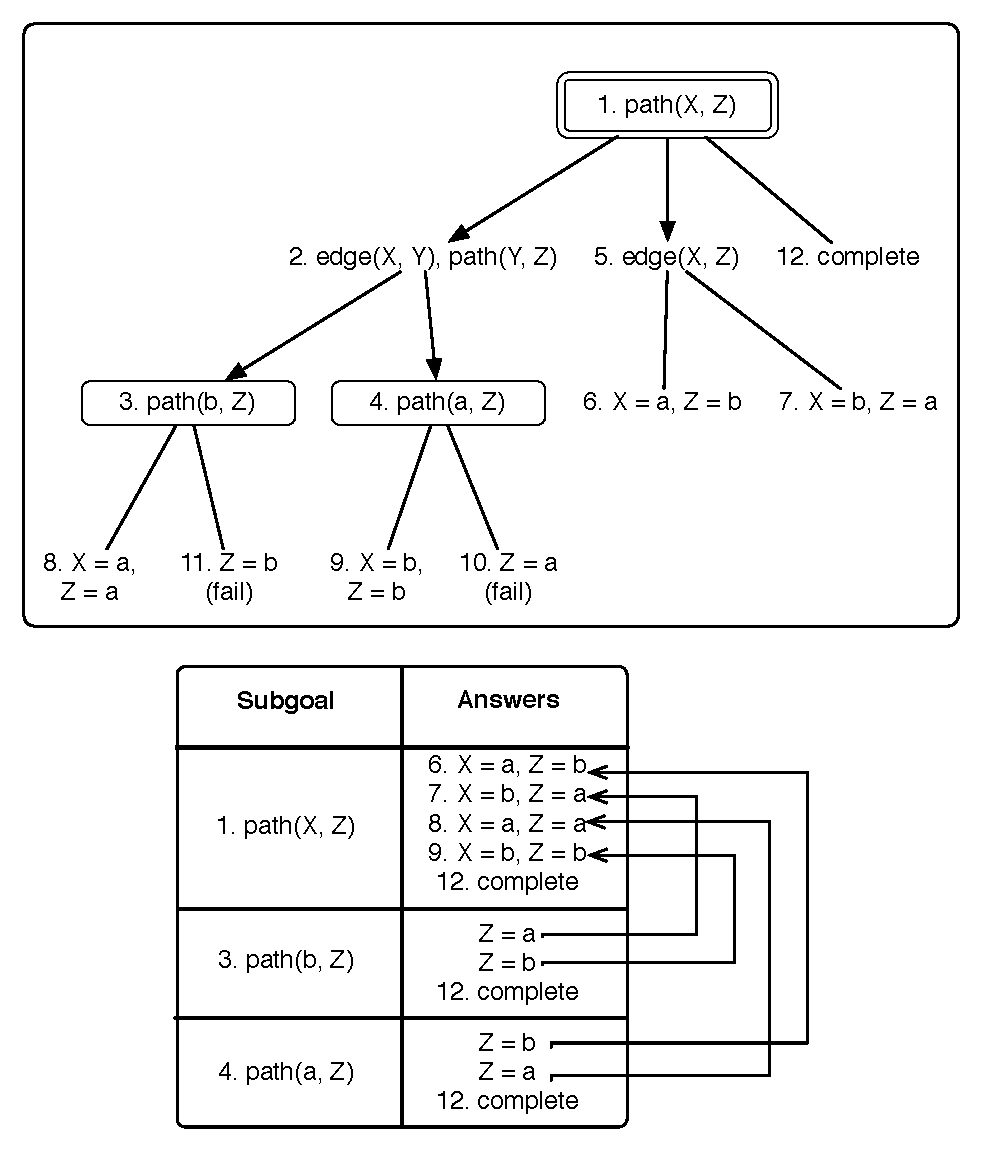
\includegraphics[scale=0.6]{tabling_path_sub.pdf}
\caption{Tabling \texttt{path(X,Z)} using call by subsumption.}
\label{fig:tabling_path_sub}
\end{figure}

At step 1 the subgoal \texttt{path(X,Z)} is called and a new generator node is created as there is no existing subgoals
in the table space that could be variant or subsuming. Being a generator node, it is evaluated using the program clauses
(step 2). The first solution for the \texttt{edge(X,Y)} predicate is evaluated using Prolog's standard rules and yields
a subgoal call to \texttt{path(b,Z)} (step 3).

In variant tabling the engine would search for a variant subgoal in the table space, thus failing and creating a
new generator node, meanwhile expanding the execution tree by means of program clause resolution. In subsumptive
tabling, the engine searches for a subsuming call, and finds \texttt{path(X,Z)}. As this subgoal is more general than
\texttt{path(b,Z)} it will generate all the answers needed for the subsumed goal. A special type of consumer called a
\textit{subsumed consumer} is thus created. This consumer knows how to retrieve the answers
that unify with the subsumed call.

As \texttt{path(X,Z)} has no answers, no answers can be consumed by \texttt{path(b,Z)}, and thus the consumer
node is suspended and execution backtracks to node 2. The second clause of \texttt{edge/2} is tried and a new tabled
subgoal is called: \texttt{path(a,Z)} (step 4). Like the subgoal \texttt{path(b,Z)}, this subgoal is subsumed by \texttt{path(X,Z)},
hence a new subsumed consumer node is created. Execution suspends once again because no answers are available and
the engine goes back to node 1 to try the second \texttt{path/2} clause (step 5).

Answers for \texttt{path(X,Z)} are found in steps 6, \texttt{\{X~=~a,~Z~=~b\}}, and 7, \texttt{\{X~=~b,~Z~=~a\}}.
They are stored in the answer set for this subgoal. Execution thus backtracks to node 1 and completion
is attempted. Node 1 verifies that node 3 and 4 have unconsumed answers and starts by resuming computation at node 3.

Node 3 being a subsumed consumer, looks up in the \texttt{path(X,Z)} answer set for answers specific to \texttt{path(b,Z)},
finding one: \texttt{\{Z~=~a\}}. At this point, the consumer marks the answer for later retrieval, so that answers can be
immediately consumed when a variant subgoal is called. Like variant tabling, the consumer keeps a last consumed answer
continuation to know which answers have already been consumed. Variable bindings for this answer are propagated and a
new answer to \texttt{path(X,Z)} is found: \texttt{\{X~=~a,~Z~=~a\}} (step 8). Node 3 tries to consume a new answer, but no
new answers are available.

Execution suspends node 3 and resumes computation at node 4. Here \texttt{path(a,Z)} begins to consume answers from
\texttt{path(X,Z)} using the subsumption mechanism. The first answer in \texttt{path(X,Z)}, \texttt{\{X~=~a,~Z~=~b\}},
unifies with the subsumed goal and is consumed. By variable propagation, a new answer for \texttt{path(X,Z)} is also
generated, \texttt{\{X~=~b,~Z~=~b\}} (step 9). Node 3 then tries to consume a new answer and finds \texttt{\{X~=~a,~Z~=~a\}}.
This new answer is added to the \texttt{path(a,Z)} table space. As the new variable bindings are propagated, a new
answer is also generated for the top subgoal, but the answer \texttt{\{X~=~b,~Z~=~a\}} is repeated (step 10), hence it
is not inserted into the table space.

Execution now suspends node 4 and resumes the the leader node, \texttt{path(X,Z)}, that will once
again attempt completion. By using the last consumed answer continuation, it verifies that node 3 has
new unconsumed answers. Execution thus resumes again at node 3.

Node 3 inspects \texttt{path(X,Z)} answer set and consumes the next matching answer, \texttt{\{X~=~b,~Z~=~b\}}.
A new answer for \texttt{path(b,Z)} is generated and variable bindings are propagated to the leader node (step 11).
However, the new answer is already stored in the table space and it is discarded.

Once again, evaluation returns to the leader node and completion is performed (step 12) as each consumer has exhausted the
available answers.

This evaluation example, when compared to variant tabling, shows a smaller execution tree with less
program clauses expanded. The subsumptive computation also took less steps to complete and a greater
reuse of answers was done between \texttt{path(X,Z)}, \texttt{path(b,Z)} and \texttt{path(a,Z)}.

Like variant tabling, the same four main operations are used when evaluating subsumptive subgoals.
These operations are very similar, with a few key differences. Operations \textit{new answer} and
\textit{completion} remain the same, while the \textit{tabled subgoal call} and \textit{answer resolution}
operations work slightly differently:

\begin{itemize}
\item The \textit{tabled subgoal call} operation represents a call to a tabled subgoal.
When a subgoal $G$ is called, a search for a subsuming subgoal $G'$ is done. If such subgoal is found,
$G$ will be resolved using \textit{answer clause resolution}, thus consuming answers from $G'$.
If no subgoal $G'$ is found, then a new entry, representing $G$, is inserted into the table space and
$G$ will be evaluated using program clause resolution.

\item The \textit{answer resolution} operation checks whether new answers from the table space are
available for consumption. Each subsumed consumer node uses an answer continuation that represents
the set of remaining answers to be consumed. Given this answer continuation, we inspect the answer trie
from the subsuming subgoal and retrieve the next answer that matches with the subsumed subgoal. Once the
answer is retrieved and loaded, the answer continuation is updated to reflect the new answer consumed.

\end{itemize}

% Although this example shows a very good performance of this method of evaluation, if we tried
% to evaluate \texttt{path(a,Z)} and then \texttt{path(X,Z)}, no reuse could be done with \texttt{path(a,Z)}
% because no previous subsuming goal was present. The more general subgoals are called first, the greater
% the reuse in call subsumption.

We next describe two known techniques that implement subsumptive tabling. These two approaches were
both implemented in XSB.

\subsection{Dynamic Threaded Sequential Automata}\label{sec:dtsa}

\textit{Dynamic Threaded Sequential Automata} (DTSA) is a data structure that provides good indexing
and incremental returning of a subset of answers from a subsuming call to a subsumed call \cite{Rao-96}.

This structure orders answers as they are generated, hence it can easily mark which answers were
already retrieved, enabling efficient retrieval of the remaining answers.

A DTSA is based on a \textit{Sequential Factoring Automaton} (SFA) \cite{Dawnson-95} but has a few more
features for dealing with fast indexing and incremental retrieving of answers.

\subsubsection{Sequential Factoring Automaton}

A SFA solves the problem of retrieving an ordered subset of answers, starting from the oldest to the
newest answer. It is an ordered tree-structure automaton and is very similar to a trie. It begins with
a root as the start state and has edges as transitions that represent unifications. Every leaf represents
a distinct term and the transitions on the path from the root to a leaf represent the operations necessary
to unify the goal with the answer at the leaf.

Apart from ordering, SFAs differ from tries in that transitions from a state may not be unique and each
transition in a trie denotes match operations, not unify operations.

\begin{figure}[ht]
  \centering
    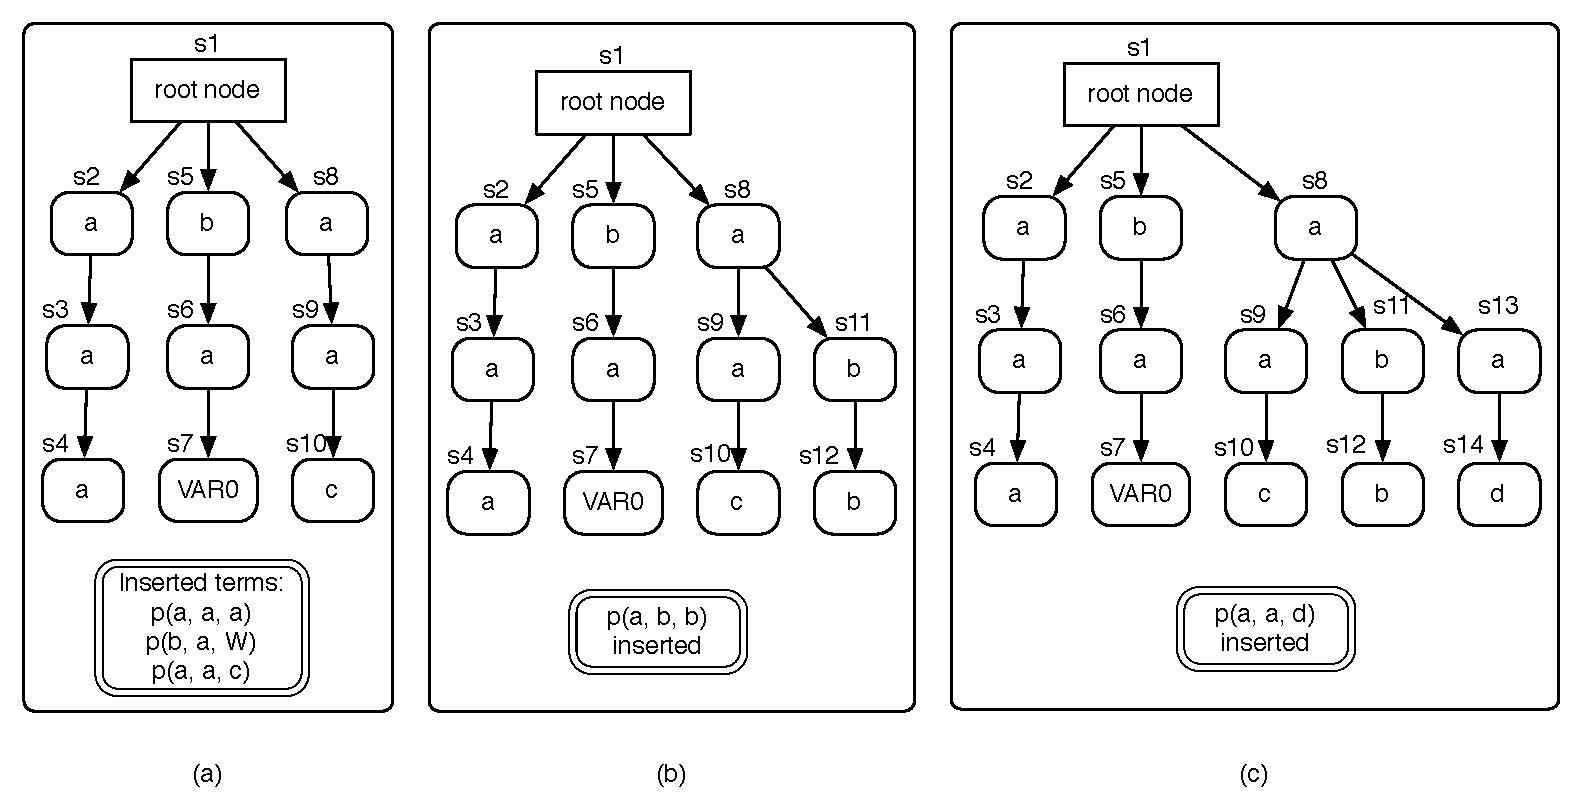
\includegraphics[scale=0.6]{sfa.pdf}
  \caption{Inserting answer terms in a SFA.}
  \label{fig:sfa_example}
\end{figure}

To insert a new term into a SFA, we must start by inserting symbols from the answer term into the root state.
In each state we verify if the \textit{last transition} $s$ matches the current term symbol $t$. If $t$ matches $s$
we take the transition and advance to the next state; if not, a new transition for $t$ is created and we advance
to the newly created state. When all term symbols $t$ are exhausted, the current state is marked as a leaf,
representing a new answer.
Figure~\ref{fig:sfa_example} represents a SFA for the subgoal \texttt{p(X,Y,Z)} and
illustrates insert operations.

When a new subgoal $G$ subsumed by the subgoal $G'$ is first called, we must determine the \textit{substitutions}
from $G'$ to the sub-terms of $G$, because only variable substitutions are inserted into a SFA.
For example, if $G'$ is \texttt{p(X,Y,Z)} and $G$ is \texttt{p(a,a,V)}, the substitutions
are \texttt{\{X~=~a,~Y~=~a,~Z~=~VAR0\}}. During unification operations, we must unify the first SFA symbol
to $a$, then to $a$ again, and finally with \texttt{VAR0}.
Once a variable is \textit{bound}, subsequent unify operations must unify with the bounded sub-term.

The unification process starts in the root state with an empty \textit{continuation stack}.
When a state $s$ is reached, the leftmost transition that unifies with the current $G$ substitution is chosen,
this is called the \textit{applicable transition}.
Before moving to the next state, we select the next applicable transition and push it on the continuation stack.
If no applicable transitions are available at state $s$ or if an answer was found, we pop a transition from
the stack and use it to search for more answers. Once no more transitions can be taken and the stack is empty, the
search process ends.

Using the SFA in Figure~\ref{fig:sfa_example} and the subgoal $G$, \texttt{p(a,a,V)}, the search mechanism starts
at the root state and is ready to retrieve all answers that unify with $G$.
The first applicable transition is $s1 \rightarrow s2$ because it unifies with the first symbol: $a$. The transition
$s1 \rightarrow s5$ can not be pushed into the continuation stack because it does not unify, but $s1 \rightarrow s8$ does.
In state $s2$ only one transition is available, thus nothing is pushed into the stack.
Transition $s2 \rightarrow s3$ unifies with symbol $a$ and we move to state $s3$. Here, the variable \texttt{VAR0} (that represents \texttt{V})
can unify with $a$, thus we can get to state $s4$, arriving at a leaf state and a new answer, \texttt{\{V~=~a\}}.

Next, the process must use the continuation stack to retrieve more answers. Transition $s1 \rightarrow s8$ is popped from the stack
and we arrive at state $s8$ with 3 available transitions. Using the previous rules, a new answer is retrieved,
\texttt{\{V~=~c\}} and the continuation stack contains the transition $s8 \rightarrow s13$.

Finally, once states $s13$ and $s14$ are visited, the process arrives at a leaf state and a new answer,
\texttt{\{V~=~d\}}, is retrieved. The process finishes and every answer that is specific to \texttt{p(a,a,V)} is found.

\subsubsection{Threaded Sequential Automata}

A \textit{Threaded Sequential Automata} extends the SFA with a concept called
\textit{equivalent states}. One state $S_1$ is equivalent to state $S_2$ if when $S_1$ is taken, $S_2$ is also
guaranteed to be visited. For example, in Figure~\ref{fig:sfa_example}, whenever states $s2$ and $s3$ are
visited, states $s8$ and $s9$ are also guaranteed to be visited, as they denote the same path.

A SFA is converted to a TSA by adding \textit{equivalence links} between equivalent states.
The SFA in Figure~\ref{fig:sfa_example} was transformed into a TSA in Figure~\ref{fig:tsa_example}.

\begin{figure}[ht]
  \centering
    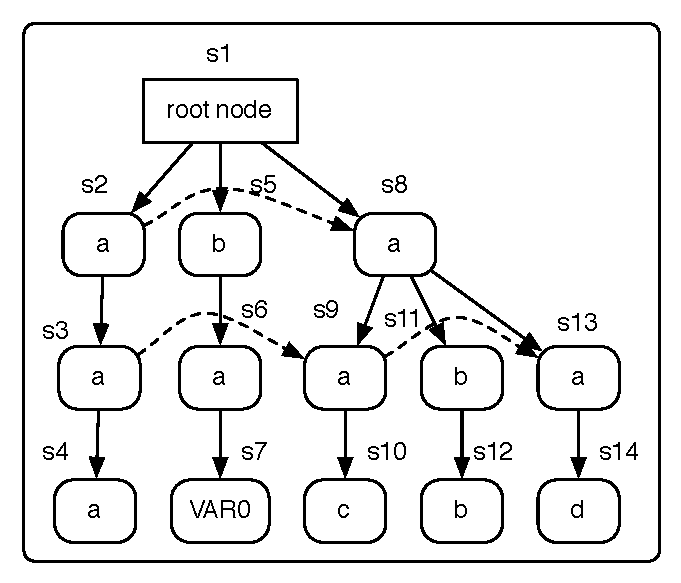
\includegraphics[scale=0.6]{tsa.pdf}
  \caption{SFA transformed into a TSA.}
  \label{fig:tsa_example}
\end{figure}

In the TSA, the concept of applicable transitions is changed. Now it is also possible to push equivalence links
into the continuation stack as if they were normal transitions. So, if we were at state $s3$ we use
the transition to $s9$ and then to $s13$ instead of going from the start state.

Although equivalence links provide an efficient indexing mechanism, they must be used with care. If not,
some situations arise where following equivalence links lead to repeated answers and answers in the
incorrect order \cite{Rao-96}. The selection of transitions must consider only \textit{safe transitions},
which reach answers that cannot be reached through the pending transitions on the stack.
So, if the process is at state $s2$ and the transition $s1$ to $s8$ is already on the
stack, we can not use the equivalence link $s2 \rightarrow s8$, as the transition $s1 \rightarrow s8$
already covers the same branch.

If we followed only safe transitions, no equivalence links would be used, hence we must check if
the usual next applicable transition covers some answers that can not be reached from using the
equivalence links on the next branch to explore, thus favoring equivalence links. Notice that at
state $s2$ we would use the equivalence link $s2 \rightarrow s8$, instead of the transition
$s1 \rightarrow s8$, as $s2 \rightarrow s8$ will cover the same answers.
 
\subsubsection{Dynamic Threaded Sequential Automata}

The previously described mechanisms only work if we have the complete set of answers for the subsuming subgoal.
A new mechanism that deals with incomplete answer sets must be devised, so that after all current answers
are retrieved, the continuation stack can be used to retrieve newly inserted answers.

The Dynamic Threaded Sequential Automata extends the TSA with special transitions in states
were new transitions can be inserted or in states were no equivalence links exist.
Figure~\ref{fig:dtsa_example} illustrates two DTSAs: (a) shows the converted TSA from Figure~\ref{fig:tsa_example}, and
(b) the resulting DTSA after inserting the answer \texttt{p(a,b,c)}.

\begin{figure}[ht]
  \centering
    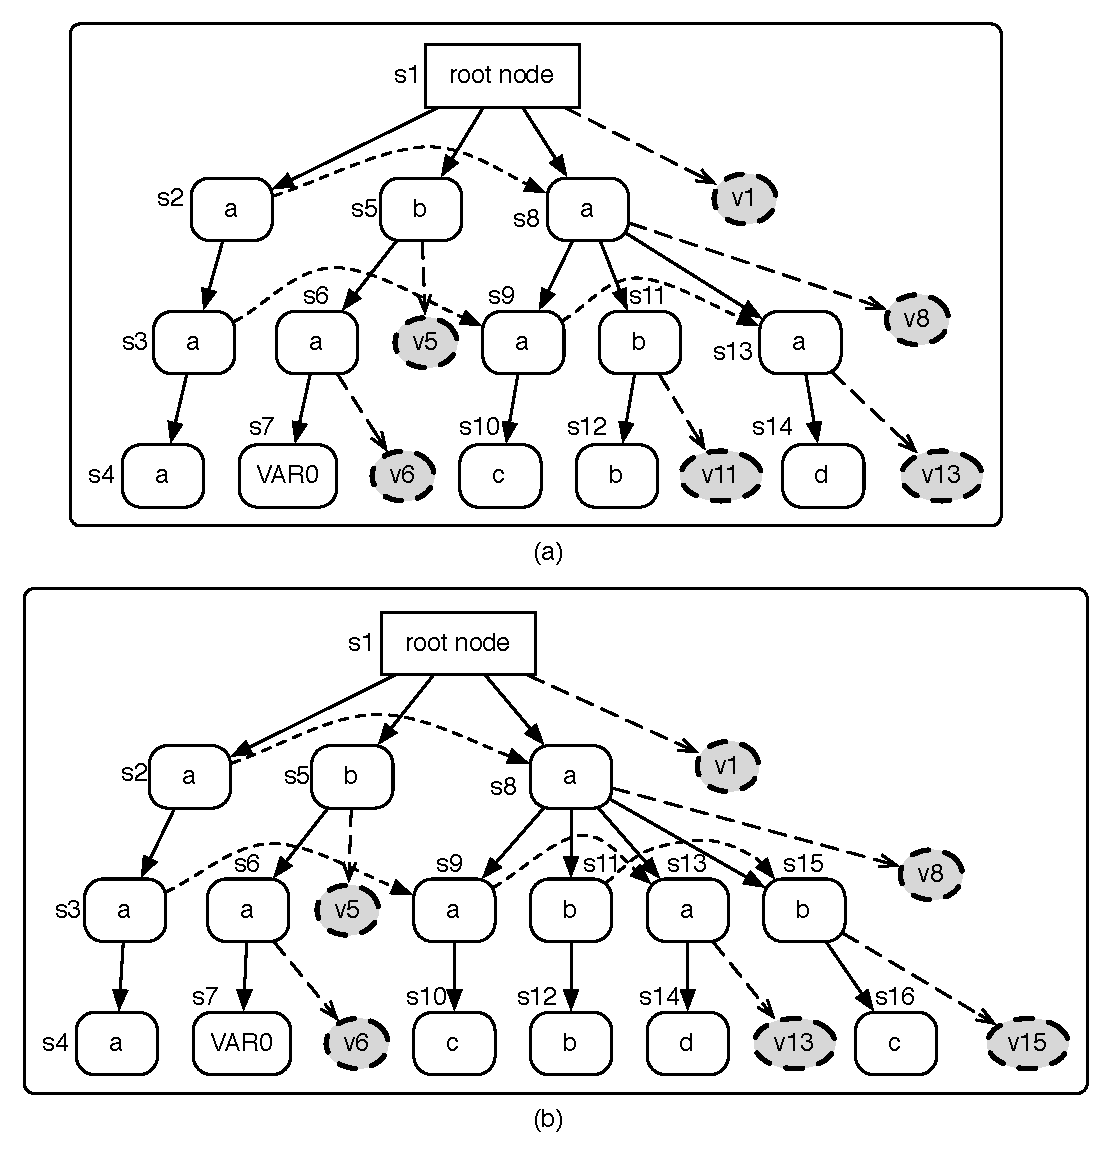
\includegraphics[scale=0.6]{dtsa.pdf}
  \caption{DTSA before and after inserting answer \texttt{p(a,b,c)}.}
  \label{fig:dtsa_example}
\end{figure}

During answer retrieval, if no answer is found and the top of the continuation stack contains
a transition to a special state, the process stops and the continuation stack is saved along the last state
visited.
Later on, when new answers must be retrieved, the last state is used to transform the stack to account for new states that
were introduced during the insertion of new terms. If the new stack contains a valid transition, it
can now be used as usual.

For example, retrieving answers to subgoal \texttt{p(a,X,c)} from the DTSA in Figure
\ref{fig:dtsa_example} (a) results in the answer \texttt{p(a,a,c)} and a continuation
formed by the last visited state $s13$ and the stack containing (from bottom to top):
$[s1~\rightarrow~v1,~s8~\rightarrow~v8,~s13~\rightarrow~v13]$.
This continuation stack contains the transitions from where it is possible that a relevant
answer will be inserted, by using either normal transitions or equivalence links.

After the new answer \texttt{p(a,b,c)} is inserted into the DTSA in Figure~\ref{fig:dtsa_example}
(b) and a consumer is resumed to consume new answers, we must check if new answers are available,
hence the continuation stack must be transformed in order to convert the virtual transitions to
instantiated transitions that may have been created after the last retrieval operation.
This stack modification is done by using the last visited state $s13$, resulting in the following
stack configuration: $[s1~\rightarrow~v1,~s8~\rightarrow~s15]$.
Now the answer \texttt{p(a,b,c)} can be easily retrieved using the transition $s8 \rightarrow s15$.
Note that the transition $s1~\rightarrow~v1$ remains unmodified as new transitions can be created
from $s1$.

\subsubsection{Table Space Organization}

This new DTSA mechanism was implemented in XSB Prolog by extending the variant engine \cite{Rao-96}.
First, each subgoal frame now contains both an answer trie and a DTSA.
Answer tries are used to check for duplicate answers and the DTSA is created lazily, when a
subsumed subgoal is first called.

Each subsumed subgoal keeps an answer return list that is built using the DTSA retrieval algorithm.
This answer list is used when variant goals of the subsumed goal are called, thus instead of using
the DTSA, answers are retrieved directly by traversing the linked list.
When a subgoal is marked as complete, the DTSA is deleted and the answer trie is converted into WAM
instructions, a feature called \textit{compiled trie code} \cite{RamakrishnanIV-99}. Answers for
subsumed goals are then retrieved using the trie instructions through unification and backtracking.

\subsection{Time Stamped Tries} \label{sec:time_stamped_tries}

\textit{Time Stamped Tries} (TST) is another mechanism that was implemented in XSB
Prolog to support tabling by call subsumption \cite{Johnson-99}.

TST is a relatively simple technique based around the idea of augmenting a trie with information about the relative time
its terms were inserted. The time of insertion of each term is called its \textit{time stamp} and is represented by a
positive integer. The time stamps are then used for incremental answer retrieval.

For each node in a trie, we extend it by including a time stamp. Along the augmented trie, the maximum time stamp
$T$ is also stored, thus allowing the insert mechanism to know the next time stamp to use for new trie paths.
An example TST for the subgoal \texttt{p(X,Y,Z)} is represented in Figure~\ref{fig:tst_1}.
By looking at the leaf nodes, the order of answer insertion
can be readily known: \texttt{p(a,a,a)}, \texttt{p(b,a,VAR0)}, \texttt{p(a,a,c)}, \texttt{p(a,b,b)} and then
\texttt{p(a,a,d)}.

\begin{figure}[ht]
  \centering
    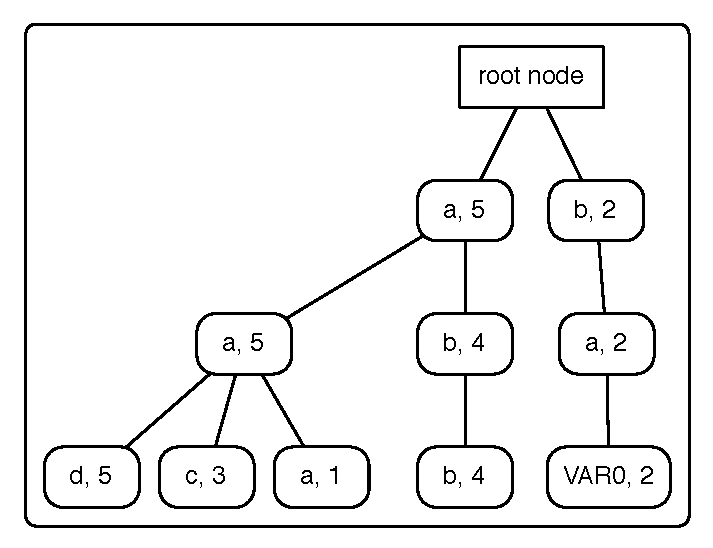
\includegraphics[scale=0.6]{tst_1.pdf}
  \caption{Time Stamped Trie for subgoal \texttt{p(X,Y,Z)}.}
  \label{fig:tst_1}
\end{figure}

\subsubsection{New Answers}

The process of inserting a new answer into a TST starts by traversing matching nodes as long the stored symbols
match the new answer. If the current symbol does not match, the process changes from search to insert mode and
new nodes are inserted to represent a new trie path. Once the leaf node is created, each node from leaf to root
is traversed and its time stamp is updated to $T + 1$.

\begin{figure}[ht]
  \centering
    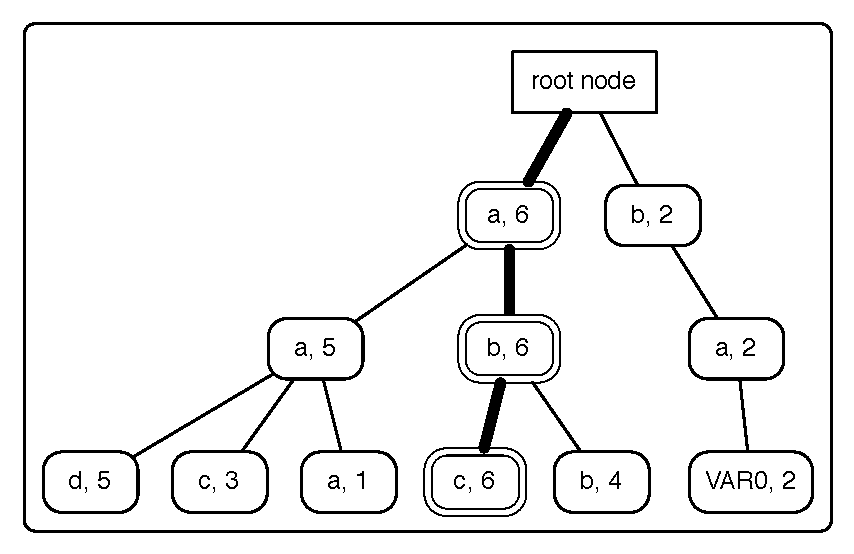
\includegraphics[scale=0.6]{tst_2.pdf}
  \caption{Time Stamped Trie from Figure~\ref{fig:tst_1} after inserting the answer \texttt{p(a,b,c)}.}
  \label{fig:tst_2}
\end{figure}

Figure~\ref{fig:tst_2} shows the TST from Figure~\ref{fig:tst_1} after a new answer \texttt{p(a,b,c)} was inserted.
Note that each node from the answer leaf node to root node was updated with time stamp 6. Apart from
the time stamps, search and insertion in TSTs work exactly the same as standard tries.

\subsubsection{Retrieving Answers}

Retrieving all answers that are specific to a subsumed subgoal $G$ from a TST with answers from subgoal $G'$
works by navigating the TST and unifying the answers against the subsumptive substitutions.
If we wanted to retrieve answers to the subgoal \texttt{p(a,a,X)} from the TST in Figure~\ref{fig:tst_2},
during the subgoal call we must determine the substitutions relative to \texttt{path(X,Y,Z)},
\texttt{\{X~=~a,~Y~=~a,~Z~=~VAR0\}}, and then we must unify the terms \texttt{[a,~a,~VAR0]} against
the trie symbols.

Like tries, TSTs only store substitutions for variables, thus we must unify
the first sub-term $a$, then $a$ again and then the variable, which unifies with any symbol.
During the unification process, if a variable appears multiple times, it must unify with
any previous sub-term assignment.

Time stamps guide the answer unification process by filtering transitions to already explored branches, where
answers were already retrieved, thus avoiding repeated answers.

The unification process that finds new answers by using a time stamp is separated from the process
of unifying the retrieved answers with the subsumed subgoal. This \textit{two-tier mechanism} is key to the space and time
efficiency of the design of TSTs \cite{Johnson-99} and allows identification of all relevant answers that have
been added since the last time a search operation was done by using the time stamp.

\subsubsection{Table Space Organization}

The table space in this technique extends the variant table space by
using TSTs instead of answer tries for subsuming goals.
 
Each subsumed subgoal frame, also represented in a subgoal trie, stores the last search time stamp $t$. The process of
incrementally searching for new answers in a TST will use $t$ and update it after the process completes.
When a subsumed subgoal is first called, $t$ is set to $0$, thus initially allowing the retrieval of all
relevant answers.

The subgoal in the subgoal trie also stores an answer return list. Each time new answers are identified, they are appended
to this linked list. The original subsumed consumer and its variant subgoals will then consume answers from it. If no
new answers can be retrieved from the list, the TST process is employed to identify more answers from the subsuming TST,
inserting them into the list.

An hashed TST node maintains a time stamp index which stores all transitions in reverse order.
It is not until a subsumed subgoal is first called that all time stamp related structures are created, thus
allowing a more efficient use of space.

Like DTSAs, the TST indexing mechanism is only used during the evaluation of subsumed calls.
For calls with completed tables, subsumed subgoals will use compiled trie instructions from the more general subgoal.

The main advantage of using TSTs instead of DTSAs is in terms of space complexity. In TSTs, the maximum table space
used is at most twice that of the variant engine, because each node can have both the time stamp and a time stamp index node.
For DTSAs, the space used is at least double, but in the worst
case can be quadratic. DTSA is at advantage in terms of speed, because it supports identification of answers and
unification in one step, thus answers can share some elementary unifications. In TSTs, identifying answers
and doing answer unification is a two step process, thus it takes more time to construct all answers. 

\section{Chapter Summary}

In this chapter we explored how the table space is efficiently designed to support
the tabling operations in a variant or a subsumption-based engine.
For the variant engine, we presented the YapTab's table space that is based on two levels
of tries, the subgoal trie and the answer trie.

Next, we discussed the two most well-known table space organizations to implement call subsumption.
The first technique is the Dynamic Threaded Sequential Automata (DTSA). This method creates a special data
structure based on tries to efficiently collect the relevant answers for a subsumed subgoal.
The second technique is the Time Stamped Trie (TST). It improves upon the previous technique by
being simpler and having reduced space needs.

In the next chapter we will discuss the algorithms and data structures used in the TST technique,
covering the algorithm used to discover subsuming subgoals and the algorithm to collect relevant
answers. Finally, we will explain how the TST mechanisms are integrated into the YapTab tabling engine to enable
call by subsumption.



\newpage
\thispagestyle{plain}
\mbox{}

\chapter{Time Stamped Tries}
In this chapter, we throughly describe the Time Stamped Tries approach
to implement a subsumptive tabling engine. This mechanism was proposed by
Ernie Johnson \textit{et al} \cite{Johnson-99} and is currently implemented in XSB.
It is based on the idea of extending each answer trie node with \textit{timestamp}
information as a means to identify new answers from old answers.

First, we start by describing the algorithms and data structures associated
with the detection of subsuming goals. Next, we explain the data structures
introduced in the answer tries to support subsumption, focusing on answer insertion
and retrieval for subsumed subgoals. Then, we describe the modifications made in the YapTab
tabling engine to support subsumptive tabling. Finally, we compare the performance of
the subsumptive YapTab against XSB, and the variant counterparts.

\section{Finding subsuming goals}\label{sec:lookup_subsuming}

Both DTSA and TSTs use a similar method that given a call trie $C$ and a subgoal $G$
is able to find a subgoal $G'$ that subsumes $G$.

The search is performed by recursively backtracking through the call trie $C$, trying
to match the node symbols with sub-terms or symbols from $G$. The process stops
once a leaf node is reached successfully.

A non-variable symbol from $G$ must only match with an identical symbol from $C$ and
these types of unifications are always tried first.
If the current trie symbol is a variable, for example \texttt{X}, on the first occurrence \texttt{X}
is bound to the respective $G$ sub-term
and match succeeds; on the next occurrences of \texttt{X}, the current sub-term from $G$ must
be identical to the term bound to \texttt{X}. Throughout the backtracking process, bound variables are
always tried before unbound variables.

Favoring constant values before variables, results in a mechanism that finds \textit{minimally subsuming calls}.
Also, if there is some variant call $G''$ in $C$, $G''$ is found before any other subgoal. If no variant 
or no subsuming call are found, it is possible to save the trie node to insert a new variant call.
This trie node is where the first backtracking occurred or when the first occurrence of
an already seen $G$ variable that could not be paired to a bound trie variable, and instead
must be bound to an unbound trie variable for the process to continue.
The new variant path is then used to keep information about the subsumed goal state in
the leaf call trie node.

\begin{figure}[ht]
  \centering
    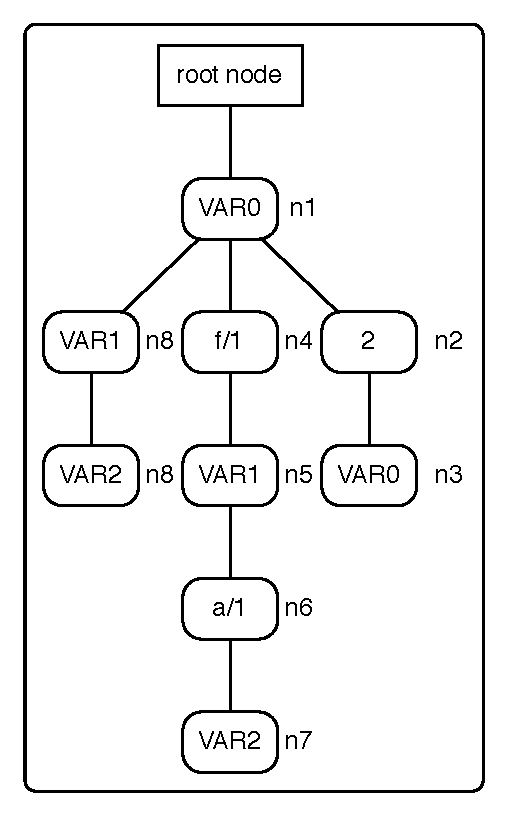
\includegraphics[scale=0.6]{sub_call_search.pdf}
  \caption{Call trie for predicate \texttt{p/3}.}
  \label{fig:sub_call_search}
\end{figure}

For illustration purposes, the Figure \ref{fig:sub_call_search} represents a call trie for the predicate \texttt{p/3}.
The first subgoal called was \texttt{p(X,2,X)}, followed by \texttt{p(X,f(Y),a(Z))} and finally \texttt{p(X,Y,Z)}.

If the subgoal \texttt{p(X,2,X)} is called once again, the algorithm described above
should find the variant subgoal represented by the leaf node $n3$. First, we unify the trie variable
\texttt{VAR0} with \texttt{X} (node $n1$), hence we must also mark the \texttt{X} variable as \textit{seen},
because if the same variable appears again it must unify with the same trie variable for a variant path
to exist. Next, \texttt{2} easily unifies with trie node $n2$ and unification proceeds. In trie node $n3$,
the current call term is \texttt{X} and we also have a variable in the trie node. As \texttt{X} was already seen before,
it must unify with \texttt{VAR0} again, it does and a variant path is found. Please note that if
the trie symbol at node $n3$ was \texttt{VAR1}, the process could proceed but a variant path would be impossible
to exist, and a subsuming subgoal would be found, as \texttt{p(VAR0,2,VAR1)} subsumes \texttt{path(VAR0,2,VAR0)}.
In this case, a variant path could be created by resuming the insert operation at node $n2$ to insert
a \texttt{VAR0} node.

For a more complex example, the subgoal \texttt{p(2,f(X),a(2))} is now called for the same call trie. First,
the algorithm tries to find a trie node with the symbol \texttt{2}, it does not and a variant path
can not be possibly found in this call trie. Next, the algorithm tries to unify with bound variables, but as the process
has just started, only unbound variables can be found and \texttt{VAR0} is unified with \texttt{2} (node $n1$).
The functor term \texttt{f/1} is the next symbol on the subgoal and the first trie node that must be tried is $n4$,
because it contains a non-variable symbol. The next term is \texttt{X} and it can unify with \texttt{VAR1} (node $n5$).
Next, the term symbol \texttt{a/1} matches with trie node $n6$ and the process proceeds. Note that if we failed
at this point, the process would backtrack to node $n2$ and node $n8$ would be tried next, which would
lead to a more general subgoal. Back to node $n6$, the last term symbol \texttt{2} can match with node $n7$, as it is the only trie
node available and it is an unbound variable. If the variable was bound, like \texttt{VAR0} for instance,
the process would check if the current term symbol unifies with the variable binding made before (\texttt{VAR0 = 2}) and
it would also succeed. As node $n7$ is a leaf node, the process finishes and a subsumptive path is found.
The following variable bindings were made: \texttt{VAR0 = 2}, \texttt{VAR1 = X}, and \texttt{VAR2 = 2}.

This algorithm uses various data structures: three auxiliary stacks, a call choice point stack,
a variable bindings vector, and variable enumerator vector. The following summarizes
each data structure: 

\begin{itemize}
  \item \textit{variable bindings vector}: saves bindings for each numbered trie variable. Starts with each position pointing to itself;
  \item \textit{variable enumerator vector}: when a never seen term variable appears it must be bound to a position in this enumerator, ensuring that it can be recognized if it appears a second time;
  \item \textit{term stack}: stores the remaining terms to be unified against trie symbols;
  \item \textit{term log stack}: stores the already matched terms. Each frame contains the top index and the top element of the term stack during frame's creation;
  \item \textit{trail stack}: stores bindings that were made during the process. It is used to untrail variables during backtracking;
  \item \textit{call choice point stack}: used to restore the search process at a certain node to explore alternatives.
\end{itemize}

During execution, two matching methods are considered: the first tries to match exact trie symbols against the current term;
the second method uses trie variables instead of exact symbols and is employed when the first method fails.
When a trie node match succeeds, matching defaults to the first method, which means
that exact matches are always tried before variables when a new \textit{trie level} is reached and variables are mainly
used when backtracking. A trie level represents a set of nodes that are linked by \texttt{sibling} links or are at
the same hash table.

\begin{figure}[ht]
  \centering
    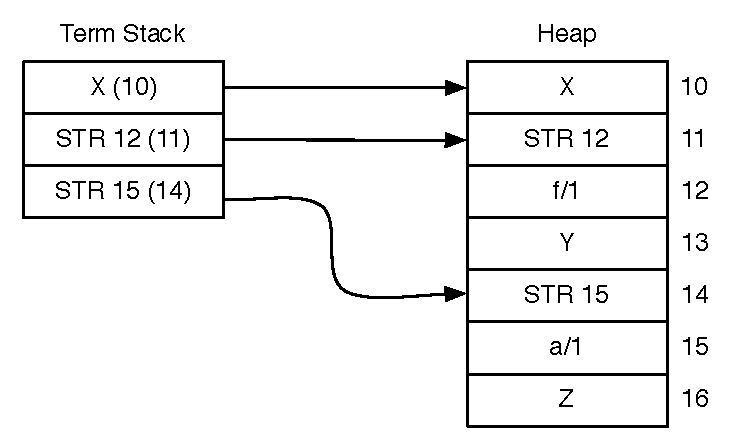
\includegraphics[scale=0.6]{lookup_subgoal_termstack_start.pdf}
  \caption{Initial term stack and heap for subgoal \texttt{p(X,f(Y),a(Z))}.}
  \label{fig:lookup_subgoal_termstack_start}
\end{figure}

The process starts by pushing the $G$ subgoal arguments, $X1, X2, ...Xn$ into the term stack, so that $X1$ is at the top
and $Xn$ at the bottom (Figure \ref{fig:lookup_subgoal_termstack_start}).
Then, the algorithm proceeds in a modified depth-first manner, trying to match the exact nodes first, and then
the variable trie nodes. The skeleton for this algorithm is presented in Figure \ref{fig:lookup_subsuming_call}.

\begin{figure}[ht]
\begin{Verbatim}[fontsize=\small]
lookup_subsuming_call(call_trie, subgoal_call) {
  match_mode = MATCH_EXACTLY
  parent = trie_root(call_trie)
  node = child(parent)
  variable_chain = NULL
  termstack_push_call(subgoal_call)

while_loop:
  while(termstack is not empty) {
    subterm = deref(termstack_pop())
    termstacklog_push(termstack_index(), termstack_top())
  
    if(subterm is atom or integer)
      match_constant(subterm)
    else if(subterm is functor or list)
      match_structured_term(subterm)
    else if(subterm is variable)
      match_variable(subterm)
  
    if(current match failed)
      if(choice point stack is empty) // no more alternatives
        return NO_PATH
      else
        (alt_node, var_chain) = ccpstack_pop_frame()
        match_mode = MATCH_TRIE_VARS
  }
  
  if variant path found
    return (VARIANT_PATH, parent)
  else
    return (SUBSUMPTIVE_PATH, parent)
}
\end{Verbatim}
\caption{Pseudo-code for \texttt{lookup\_subsuming\_call}.}
\label{fig:lookup_subsuming_call}
\end{figure}

\subsubsection{Call choice point stack}

The call choice point stack (Figure \ref{fig:call_choice_point_stack}) contains alternative
search paths to use if the process fails somewhere in the trie.
Each stack frame can restore the search at a given node by restoring all the auxiliary stacks state at the time
of the call frame creation.

\begin{figure}[ht]
  \centering
    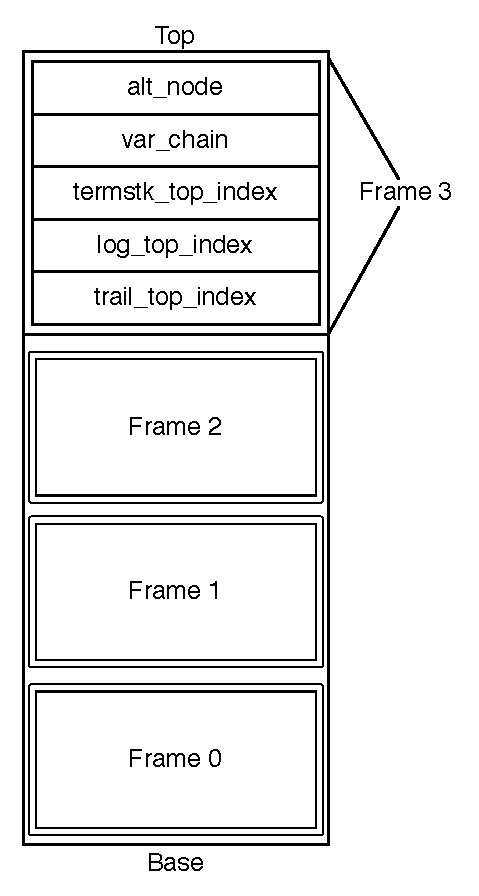
\includegraphics[scale=0.6]{call_choice_point_stack.pdf}
  \caption{Call choice point stack organization.}
  \label{fig:call_choice_point_stack}
\end{figure}

Each frame contains the next trie node to explore (\texttt{alt\_node}),
the current variable chain (\texttt{var\_chain}),
and the following stack indexes during frame creation:
the top of the term stack (\texttt{termstk\_top\_index}),
the top of the term log stack (\texttt{log\_top\_index}),
and the top of the trail stack (\texttt{trail\_top\_index}).
The function \texttt{ccpstack\_push\_frame} (Figure \ref{fig:ccpstack_push_frame})
is used to create a new frame from the computation state.

\begin{figure}[ht]
\begin{Verbatim}[fontsize=\small]
ccpstack_push_frame(alt_node, var_chain) {
  CCPFrame new_frame = new CPPFrame()
  new_frame.alt_node = alt_node
  new_frame.var_chain = var_chain
  new_frame.termstk_top_index = termstack_top - termstack_base + 1
  new_frame.log_top_index = termstacklog_top - termstacklog_base - 1
  new_frame.trail_top_index = trail_top - trail_base
  ccpstack_push(new_frame)
}
\end{Verbatim}
\caption{Pseudo-code for \texttt{ccpstack\_push\_frame}.}
\label{fig:ccpstack_push_frame}
\end{figure}

When popping a frame from the stack, the state of the auxiliary stacks and the other data
structures is restored. Consider a computational state $S1$ that pushed unto the stack
the frame $F1$. Given that we are at state $S2$ and we need to backtrack to the previous state, $S1$,
first we need remove $F1$ from the stack and use the frame's information to restore $S1$.

Any terms that were popped from the term stack from $S1$ to $S2$, which were
stored in the term log stack must be restored back into the term stack.
Then, any bindings made from $S1$ to $S2$ must be untrailed, which is
accomplished by \textit{unwinding} the trail stack. The unwind process untrails
any trie variables bound to the trie variable bindings vector
and any term variable which may have been made to point to the variable enumerator. 

Finally the alternative node and
the variable chain at state $S1$ is also restored. All this is accomplished by the
function \texttt{ccpstack\_pop\_frame} (Figure \ref{fig:ccpstack_pop_frame}).

\begin{figure}[ht]
\begin{Verbatim}[fontsize=\small]
ccpstack_pop_frame() {
  CCPFrame top_frame = ccpstack_pop()
  termstacklog_unwind(top_frame.log_top_index)
  termstack_set_top_of_stack(top_frame.termstk_top_index)
  trail_unwind(top_frame.trail_top_index)
  
  return (top_frame.alt_node, top_frame.var_chain)
}
\end{Verbatim}
\caption{Pseudo-code for \texttt{ccpstack\_push\_frame}.}
\label{fig:ccpstack_pop_frame}
\end{figure}

The node associated with $S2$ and its successors are never visited again and
the process continues until a leaf node is reached or the call choice point stack
is exhausted and the entire trie is visited, yielding no results.

\subsubsection{Matching constants}

The \texttt{match\_constant} function is called when the next term from the term stack is a integer or an
atom. First, in phase \textbf{(1)}, the function checks if the match method is to exactly match the
subterm constant against a trie symbol, which means
that this is the first time this trie level is explored. If the current trie level is represented by a simple
linked list, both \texttt{node} and \texttt{var\_chain} point to the start of the chain, but if the trie level
is an hash table, \texttt{node} will point to the symbol bucket and \texttt{var\_chain} to the variable
bucket, which usually is the first bucket.

\begin{figure}[ht]
\begin{Verbatim}[fontsize=\small]
match_constant(constant) {
  if match_mode == MATCH_EXACTLY // (1)
    (node, var_chain) = set_node_and_var_chain(constant)
    match_node = find_matching_node(constant, node)
    if match_node is not NULL
      conditionally_create_choice_point(var_chain)
      descend_node(match_node)
    else // no match found
      node = var_chain
      no_variant_found(parent)
  // no exact match, try bound trie variables (2)
  match_node = find_bound_trie_var(constant, node)
  if match_node is not NULL
    ccpstack_push_frame(next(match_node), var_chain)
    descend_node(match_node)
  // no bound trie variable found, use unbound trie variables (3)
  match_node = find_unbound_trie_var(var_chain)
  if match_node is not NULL
    bind_trie_var(match_node, constant)
    descend_node(match_node)
}
\end{Verbatim}
\caption{Pseudo-code for \texttt{match\_constant}.}
\label{fig:match_constant}
\end{figure}

The function \texttt{find\_matching\_node} iterates a linked list and locates a trie node that contains the
\texttt{constant} symbol. If this node is found we conditionally create a
new choice point (Figure \ref{fig:conditionally_create_choice_point}), that is
we try to find a node with a variable that can be used when backtracking. At this point, only
trie variables can be explored as only one node with the matched symbol exists at this level.

\begin{figure}[ht]
\begin{Verbatim}[fontsize=\small]
conditionally_create_choice_point(var_chain) {
  foreach(node in var_chain)
    if(is_trie_var(node))
      ccpstack_push_frame(node, node)
      return
}
\end{Verbatim}
\caption{Pseudo-code for \texttt{conditionally\_create\_choice\_point}.}
\label{fig:conditionally_create_choice_point}
\end{figure}

Please note that the found variable node is used as the alternative node in this choice point
and as the variable chain, which will be used to try bound and unbound trie nodes, when backtracking happens.

To descend into a node when a matching succeeds the function \texttt{descend\_node} (Figure \ref{fig:descend_node})
is used. It sets the current \texttt{node} and \texttt{parent} information, sets the matching mode for a new trie level
and changes the program flow to the main \texttt{lookup\_subsuming\_call} while loop. But,
if an exact match fails, we know that the current path cannot be variant of the called subgoal, and we call
\texttt{no\_variant\_found} with the parent node as argument.

\begin{figure}[ht]
\begin{Verbatim}[fontsize=\small]
descend_node(target_node) {
  parent = target_node
  node = child(target_node)
  match_mode = MATCH_EXACTLY
  goto while_loop
}
\end{Verbatim}
\caption{Pseudo-code for \texttt{descend\_node}.}
\label{fig:descend_node}
\end{figure}

Phase \textbf{(2)} of \texttt{match\_constant} can be reached by a failed exact match or by backtracking
(remember that the match mode changes to \texttt{MATCH\_TRIE\_VARS} when backtracking). In this step
we call \texttt{find\_bound\_trie\_var} that will iterate over the \texttt{node} chain to look for
\textit{bound trie variables}. When inserting new subgoals on the call trie, each new trie variable
along a path is marked, so it is easy to check for old variables, which have already been bound
to some term before arriving at the current node. The variable binding can be retrieved by
checking the trie variable bindings position for this variable number, which points to an heap term.
Given that we are trying to match a constant symbol, we verify if the bound term matches our symbol.
In this case, we create a new choice point for the sibling node of the matched trie variable, and use
the currently set variable chain.

Finally, if phase \textbf{(1)} and \textbf{(2)} fail, we try to match our constant against an unbound trie variable
(Figure \ref{fig:find_unbound_trie_var}).
Phase \textbf{(3)} can be also reached by a failed exact and bound trie variable match or by subsequent backtrack
attempts. If a node is found, we bind the variable position on the trie variable bindings
vector to point to the new constant. This position is also trailed on the trail stack, so that it can be untrailed
if backtracking is executed.

\begin{figure}[ht]
\begin{Verbatim}[fontsize=\small]
find_unbound_trie_var(var_chain) {
  foreach(node in var_chain)
    if(is_variable(node) and is_new_variable(node))
      return node
}
\end{Verbatim}
\caption{Pseudo-code for \texttt{find\_unbound\_trie\_var}.}
\label{fig:find_unbound_trie_var}
\end{figure}

\subsubsection{Matching structured terms}

When a structured term appears on the term stack, either a functor or a list, the matching process works
just like constants, except the functor or list arguments must be pushed unto the term stack after an exact
match is found (Figure \ref{fig:match_structured_term}).

\begin{figure}[ht]
\begin{Verbatim}[fontsize=\small]
match_structured_term(term) {
  if match_mode == MATCH_EXACTLY // (1)
    (node, var_chain) = set_node_and_var_chain(term)
    match_node = find_matching_node(term, node)
    if match_node is not NULL
      termstack_push_arguments(term)
      conditionally_create_choice_point(var_chain)
      descend_node(match_node)
    else // no match found
      node = var_chain
      no_variant_found(parent)
  // no exact match, try bound trie variables (2)
  match_node = find_bound_trie_var(term, node)
  if match_node is not NULL
    ccpstack_push_frame(next(match_node), var_chain)
    descend_node(match_node)
  // no bound trie variable found, use unbound trie variables (3)
  match_node = find_unbound_trie_var(var_chain)
  if match_node is not NULL
    bind_trie_var(match_node, term)
    descend_node(match_node)
}
\end{Verbatim}
\caption{Pseudo-code for \texttt{match\_structured\_term}.}
\label{fig:match_structured_term}
\end{figure}

Figure \ref{fig:match_functor} shows the evolution of the term stack for finding
a subsuming goal for the subgoal \texttt{p(a,f(b))}. Step \textbf{(1)} shows the initial 
term stack, followed by a match of the term on top of the stack, \texttt{a}, against \textbf{VAR0}.
As it is an unbound trie variable, the first position of the variable bindings vector is
bound to the target term, \texttt{a}.
In step \textbf{(2)}, we try to match the functor \texttt{f/1} against node \textbf{(b)}, but we fail.
Node \textbf{(c)} succeeds as it is an exact match and the functor argument, \texttt{b}, is pushed on
the term stack. In step \textbf{(3)}, \texttt{b} matches against \texttt{b}, and we find a subsuming call:
\texttt{p(VAR0,f(b))}.

\begin{figure}[ht]
  \centering
    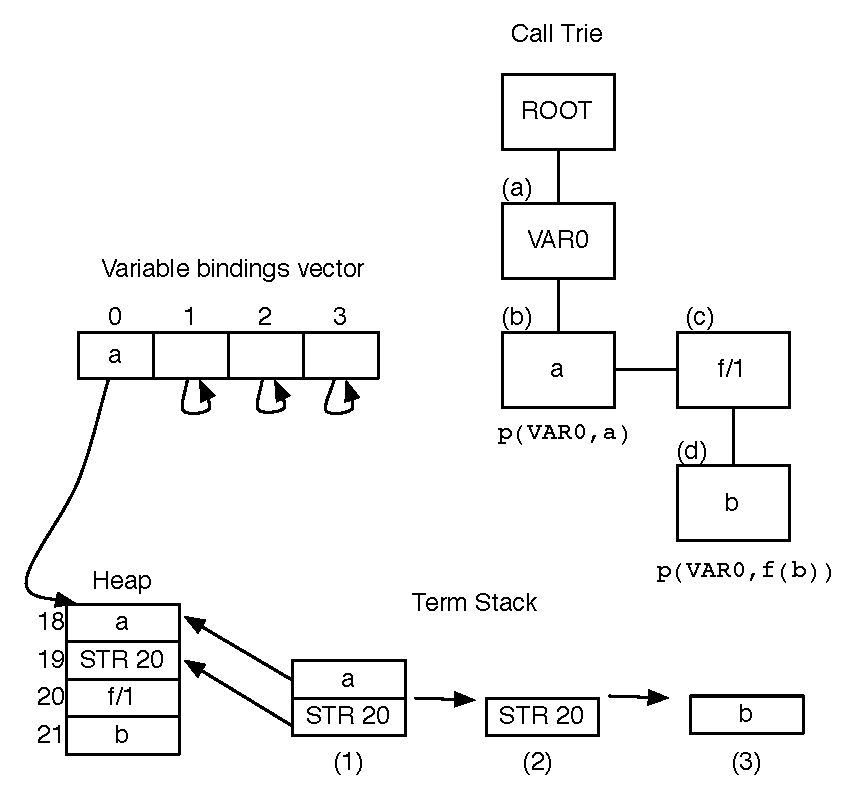
\includegraphics[scale=0.6]{match_functor.pdf}
  \caption{Finding a subsuming goal for subgoal \texttt{p(a,f(b))}.}
  \label{fig:match_functor}
\end{figure}

\subsubsection{Matching variables}

The last case for matching terms are variables. Because we are trying to find a more general goal,
a term variable must only be matched or bound against a trie variable and nothing else. More, a
never seen variable must match only with an unbound trie variable, consider the case of trying to
match \texttt{p(X,Y)} against \texttt{p(X,X)}, the first call variable could match the first trie variable,
but the call variable \texttt{Y} must be matched against an unbound variable, thus the next trie variable
(in this case \texttt{VAR0}) cannot be matched, because it was already bound to another variable.
Please note that \texttt{p(X,X)} is subsumed by \texttt{p(X,Y)} and not the other way around.

To recognize already seen call variables, we bind them to the variable enumerator array, indexed
by the corresponding trie variable number and use the trail stack to trail them.
When such call variable must be matched again with a
trie variable, we first try to match it with the same trie variable, and if we fail to find such trie
variable, we use an unbound trie variable, thus, we avoid binding two different call variables to the same
trie variable.

\begin{figure}[ht]
\begin{Verbatim}[fontsize=\small]
match_variable(term) { // term represents a variable on the heap
  if match_mode == MATCH_EXACTLY
    if node is not NULL and is_hash_table(node)
      node = var_chain = hash_bucket(node, VARIABLE_BUCKET)
    else
      var_chain = node
    if variable is not marked(term)
      // variable not seen before
      // only one new trie variable per level, no choice point needed
      foreach(test_node in node) {
        if is_trie_var(test_node) and is_new_variable(test_node)
          bind_trie_var(test_node, term)
          mark_prolog_var(term, var_index(test_node))
          descend_node(test_node)
      no_variant_found(parent)
      backtrack
  // variable has been seen before
  foreach(test_node in node)
    if is_trie_var(test_node) and !is_new_variable(test_node)
      if identical_terms(trie_var_bindings[test_node], term)
        ccpstack_push_frame(next(test_node), var_chain)
        descend_node(test_node)
  // variant path is not possible here
  no_variant_found(parent)
  // match against unbound trie variable
  foreach(test_node in var_chain)
    // only one new trie variable per level, no choice point needed
    if is_trie_var(test_node) and is_new_variable(test_node)
      bind_trie_var(test_node, trie_var_bindings[prolog_var_index(term)])
      descend_node(test_node)
}
\end{Verbatim}
\caption{Pseudo-code for \texttt{match\_variable}.}
\label{fig:match_variable}
\end{figure}

The pseudo-code to match against a variable is displayed in Figure
\ref{fig:match_variable}. From it, we can conclude that a variant path
cannot be found when: (1) a new trie variable cannot be found
for a new call variable, (2) we cannot match an already seen
call variable against the same trie variable already bound to it.

\subsubsection{Variant continuations}

The \texttt{lookup\_subsuming\_call} algorithm has the ability to find a
minimally subsuming call and if a variant path exists, it will be found.

A \textit{variant continuation} is built when the algorithm detects that a variant path of the
called subgoal cannot be found on the call trie during the search process.
A variant continuation stores all the needed information to later resume
the algorithm that creates a variant path starting from the last node where the
search for a variant path has failed.

In the above pseudo-code we used the function \texttt{no\_variant\_found} to create
a variant continuation. This function creates a continuation the first time it is called.

The continuation stores the node from where the rest of the variant path is created,
the term stack at creation's time and all the bindings made to the call variables
to the variable enumerator vector that were trailed on the trail stack.

\begin{figure}[ht]
  \centering
    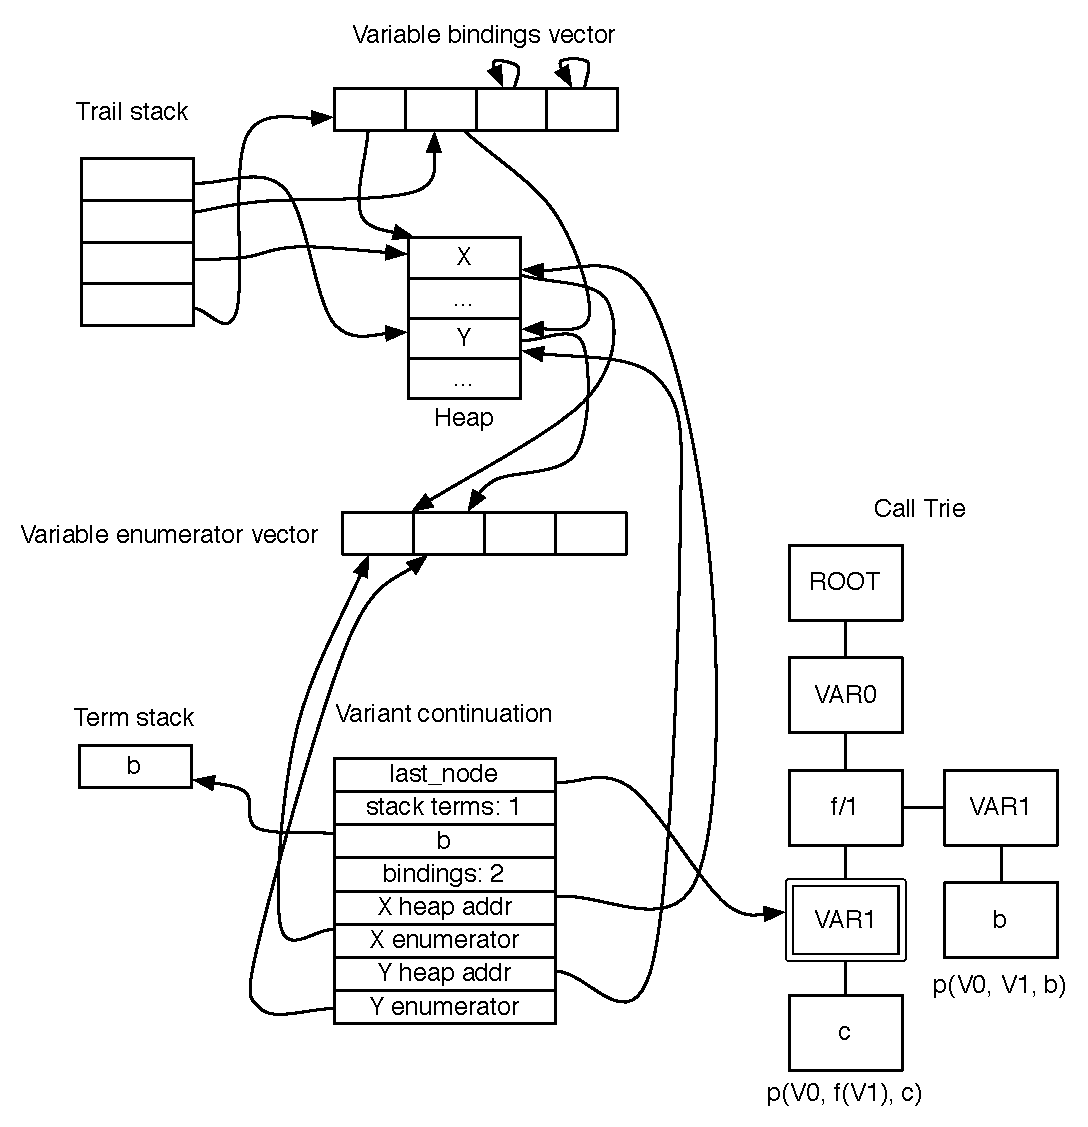
\includegraphics[scale=0.6]{variant_continuation.pdf}
  \caption{Creation of an variant continuation for subgoal \texttt{p(X,f(Y),b)}.}
  \label{fig:variant_continuation}
\end{figure}

Figure \ref{fig:variant_continuation} shows a variant continuation that is built
after the match process failed at node \texttt{c}. If a variant path
for subgoal \texttt{p(X,f(Y),b)} needs to be created: the term stack is restored
with the terms saved on the continuation; the trail stack is initialized with
the two variable heap addresses and each variable is bound to the saved
enumerator addresses. The variable enumerator vector is used during the insertion
of variant paths to detect if a variable was already seen and easily compute its number by
looking at the enumerator position. If it is a new variable, a new trie variable is generated,
and the call variable is pushed on the trail stack and bound to the corresponding enumerator address. 

\section{Answer Templates}

In a variant engine, a substitution factor
represents an array of unique variables which exist in the terms of the argument registers.
These variables are bound to terms when consuming answers from an answer trie.
Figure \ref{fig:answer_template_generator} shows a substitution factor that is constructed
on the local stack below the choice point, in this case a generator choice point.
Note that the substitution factor size (2) is also stored.

\begin{figure}[ht]
  \centering
    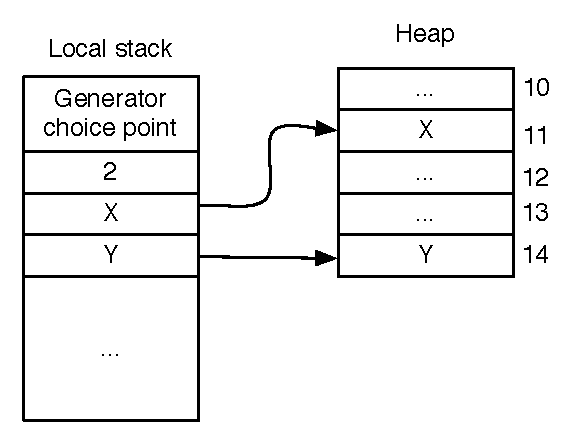
\includegraphics[scale=0.6]{answer_template_generator.pdf}
  \caption{Answer template for generator \texttt{p(X,f(Y))}.}
  \label{fig:answer_template_generator}
\end{figure}

When using call by subsumption, the same factor is used for
subgoals which do not consume from more general subgoals: \textit{generator subgoals}
and variant consumers of generator subgoals.
We call this type of substitution factor a \textit{generator answer template}.

For subgoals with more general subgoals, variants of consumer subgoals and consumers
which consume from consumer subgoals, the answer template must specialize the generator answer template
from the most general subgoal, and is called a \textit{consumer answer template}.
If a generator subgoal \texttt{p(X,f(Y))} exists and the consumer subgoal \texttt{p(a,f(g(2, X)))}
is called, the answer template illustrated on Figure \ref{fig:answer_template_consumer} is built.
Consumer answer templates have the exact same size of generator answer templates
and instead of being composed only of variables, can also be composed with other types of sub-terms.

\begin{figure}[ht]
  \centering
    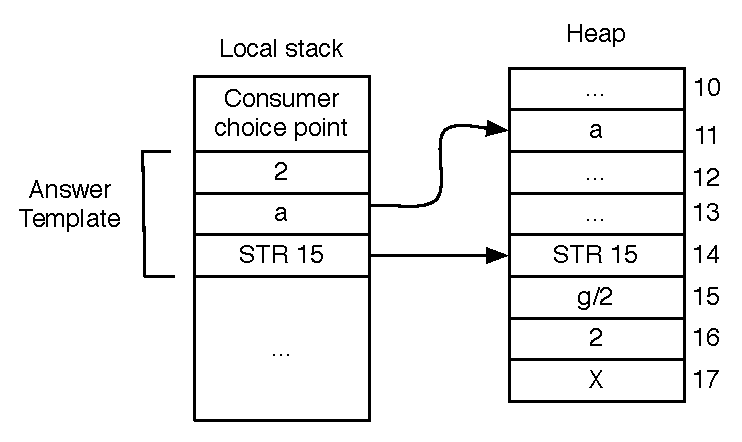
\includegraphics[scale=0.6]{answer_template_consumer.pdf}
  \caption{Answer template for consumer \texttt{p(a,f(g(a,X)))}.}
  \label{fig:answer_template_consumer}
\end{figure}

The construction of answer templates is done when trying to find a general goal on the call trie.
If no subsuming subgoal frame is found, a generator answer template is built. If a subsuming subgoal
is found, the subgoal frame $S$ can be either:

\begin{enumerate}
  \item ... a generator: the answer template is constructed by iterating over the trie variable bindings vector (Figure \ref{fig:extract_template_from_lookup});
  \item ... a consumer: the answer template is reconstructed by using the generator subgoal frame $S'$ from $S$ as we will consume from the generator $S'$ and not $S$. \texttt{reconstruct\_template\_for\_producer} uses another stack, the symbol stack, to push all the trie symbols from the general subgoal path, from leaf to root. The term stack is used to push all the called subgoal arguments that will be matched against the trie symbols. The answer template is then built by matching the new trie variables against the current term on the term stack. Note that when a functor or list symbol appears on the symbol stack the current term is also certainly a functor or list, because the called subgoal specializes the more general subgoal.
\end{enumerate}

\begin{figure}[ht]
\begin{Verbatim}[fontsize=\small]
extract_template_from_lookup(answer_template) {
  total = 0
  foreach(binding in trie variable bindings vector)
    *answer_template-- = binding
    total++
  *answer_template = total
  return answer_template
}
\end{Verbatim}
\caption{Pseudo-code for \texttt{extract\_template\_from\_lookup}.}
\label{fig:extract_template_from_lookup}
\end{figure}

\begin{figure}[ht]
\begin{Verbatim}[fontsize=\small]
reconstruct_template_for_producer(subgoal_call, generator_sf_fr, answer_template) {
  symbol_stack_push_path(leaf_node(generator_sf_fr))
  
  termstack_push_call(subgoal_call)
  
  total = 0
  while(termstack is not empty) {
    subterm = deref(termstack_pop())
    symbol = symbol_stack_pop()
    if is_trie_var(symbol) and is_new_variable(symbol)
      *answer_template-- = subterm
      total++
    else if is_functor(symbol) or is_list(symbol)
      termstack_push_arguments(subterm)
  }
  
  *answer_template = total
  return answer_template
}
\end{Verbatim}
\caption{Pseudo-code for \texttt{reconstruct\_template\_for\_producer}.}
\label{fig:reconstruct_template_for_producer}
\end{figure}

\section{Time stamped tries}

A time stamped node extends an answer trie node with timestamp information, thus
each node contains the following fields: \texttt{symbol}, \texttt{child}, \texttt{parent}, \texttt{sibling}
and \texttt{timestamp}. For implementation and algorithmic purposes, each node also needs a bit field,
\texttt{status}, that describes some node properties that will be described shortly.

Insertion of an answer $S$ into a TST can be divided into two phases:

\begin{enumerate}
  \item Finding a more general answer $S'$ on the trie.
  \item Inserting $S$ if $S'$ could not be found.
\end{enumerate}

Step (1) uses the algorithm described in Section \ref{sec:lookup_subsuming} to discover a more general answer, or,
to find a \textit{repeated answer}, which is a variant of $S$.
Step (2) is executed when (1) fails and uses a variant continuation to resume the insertion of the answer
on the last node a variant answer could be found during the search for $S'$.

\begin{figure}[ht]
\begin{Verbatim}[fontsize=\small]
subsumptive_answer_search(trie_root, ans_vector, maintain_tsi)
  (path, leaf) = lookup_subsuming_call(trie_root, ans_vector) // step 1
  if path == NO_PATH
    // step 2
    leaf = tst_insert(trie_root, restore_variant_continuation(), maintain_tsi)
  return leaf
}
\end{Verbatim}
\caption{Pseudo-code for \texttt{subsumptive\_answer\_search}.}
\label{fig:subsumptive_answer_search}
\end{figure}

The function \texttt{subsumptive\_answer\_search} (Figure \ref{fig:subsumptive_answer_search})
implements the two phase process and needs three arguments: the root of the answer trie \texttt{trie\_root},
the answer as a vector of terms \texttt{ans\_vector}, and a boolean argument, \texttt{maintain\_tsi}.

When a chain of sibling nodes becomes larger then a threshold value, we dynamically index the nodes through an hash table to provide direct node access and therefore optimize the search. Given that an hash table
can have a large number of answer nodes, we maintain a double linked list of answer nodes that we keep on the hash
table, in a decreasing order of the time stamp values. This linked list is called a \textit{time stamped index}.
Besides the usual double linked list pointers, each index node contains a pointer to the answer node
and the timestamp for the answer node. Each answer node indexed in the hash table has a different use
for the \texttt{timestamp} field: instead of containing a positive integer, contains a pointer to the respective index node. Figure \ref{fig:hash_table_tst} illustrates an hash table and its time stamp index.

\begin{figure}[ht]
  \centering
    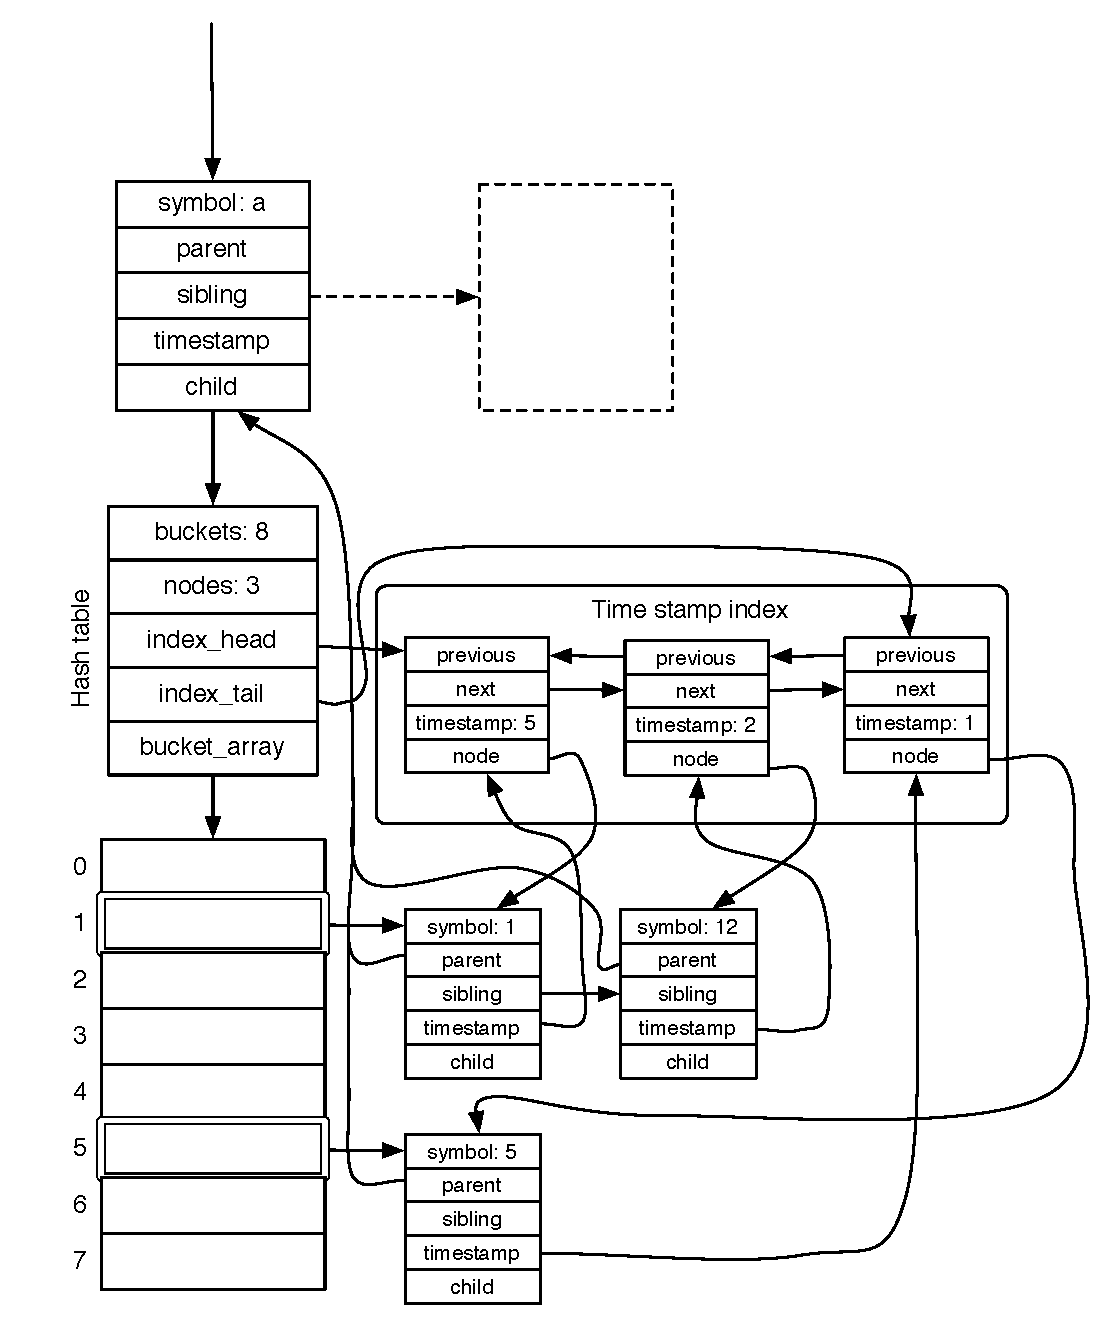
\includegraphics[scale=0.6]{hash_table_tst.pdf}
  \caption{Indexing nodes through an hash table and time stamp indexes.}
  \label{fig:hash_table_tst}
\end{figure}

The argument \texttt{maintain\_tsi} on \texttt{subsumptive\_answer\_search} indicates wether
time stamp indexes exist on the trie and if they need to be maintained.

\subsubsection{Inserting new answers}

Once the variant continuation is restored, the rest of the answer path can be inserted on the trie starting
from the restored node. Inserting is then a simple operation because no checking for equal trie symbols is required.
The first symbol will be inserted either: (1) into a childless parent (ie, the trie root); (2) into a node where
we must append the new node in the sibling chain list; (3) into an hashed node, where the symbol must go be indexed.
Every other symbol will be inserted on a childless parent.

\begin{figure}[ht]
\begin{Verbatim}[fontsize=\small]
tst_insert(trie_root, node, maintain_tsi) {
  symbol = process_term_stack()
  if child(node) == null
    // inserting on the root
    node = tst_add_symbol(node, symbol)
  else if is_hash_table(node)
    node = tst_hash_table_add_symbol(node, symbol, maintain_tsi)
  else
    node = tst_insert_symbol(node, symbol, maintain_tsi)
  
  // at this point, just add nodes on childless parents
  while(termstack is not empty) {
    symbol = process_term_stack()
    node = tst_add_symbol(node, symbol)
  }
  
  update_timestamps(node, trie_root, maintain_tsi)
  return node
}
\end{Verbatim}
\caption{Pseudo-code for \texttt{tst\_insert}.}
\label{fig:tst_insert}
\end{figure}

Function \texttt{tst\_insert} (Figure \ref{fig:tst_insert}) does the job of inserting
all the terms contained in a stack of terms into the trie, starting from \texttt{node}.
The difference between functions \texttt{tst\_add\_symbol} and \texttt{tst\_insert\_symbol}
is that the former inserts symbols on childless nodes and the later on nodes with children.

The function \texttt{process\_term\_stack} pops a term from the term stack and converts the term
to a trie representation, which is usually called a \textit{symbol}. If the term is a functor or a list,
the arguments are pushed into the stack of terms, to be processed next.

\begin{figure}[ht]
  \centering
    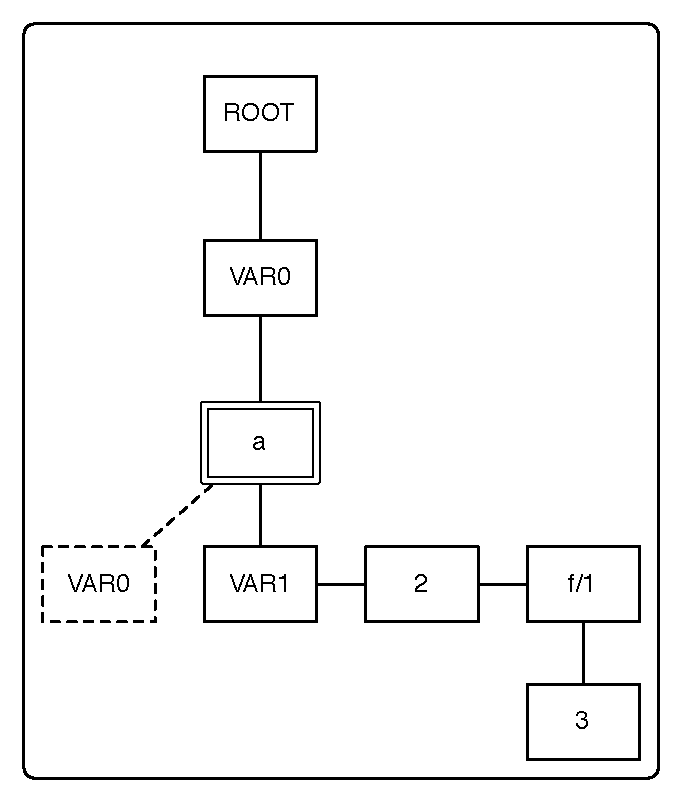
\includegraphics[scale=0.45]{tst_insert.pdf}
  \caption{Inserting answer $\{$\textit{VAR0, a, VAR0}$\}$.}
  \label{fig:tst_chain_insert}
\end{figure}

While appending a new node in a sibling listdoes not involve any
time stamp index (see Figure \ref{fig:tst_chain_insert}), indexing a new node into an hash table does,
because hash tables can index nodes by the time stamp. Figure \ref{fig:hash_table_insert}
illustrates the indexing and insertion of a symbol (25) and the creation of the respective
index node. Note that the \texttt{index head} field was changed to point to the new index node, which
is the node with the greatest time stamp.

\begin{figure}[ht]
  \centering
    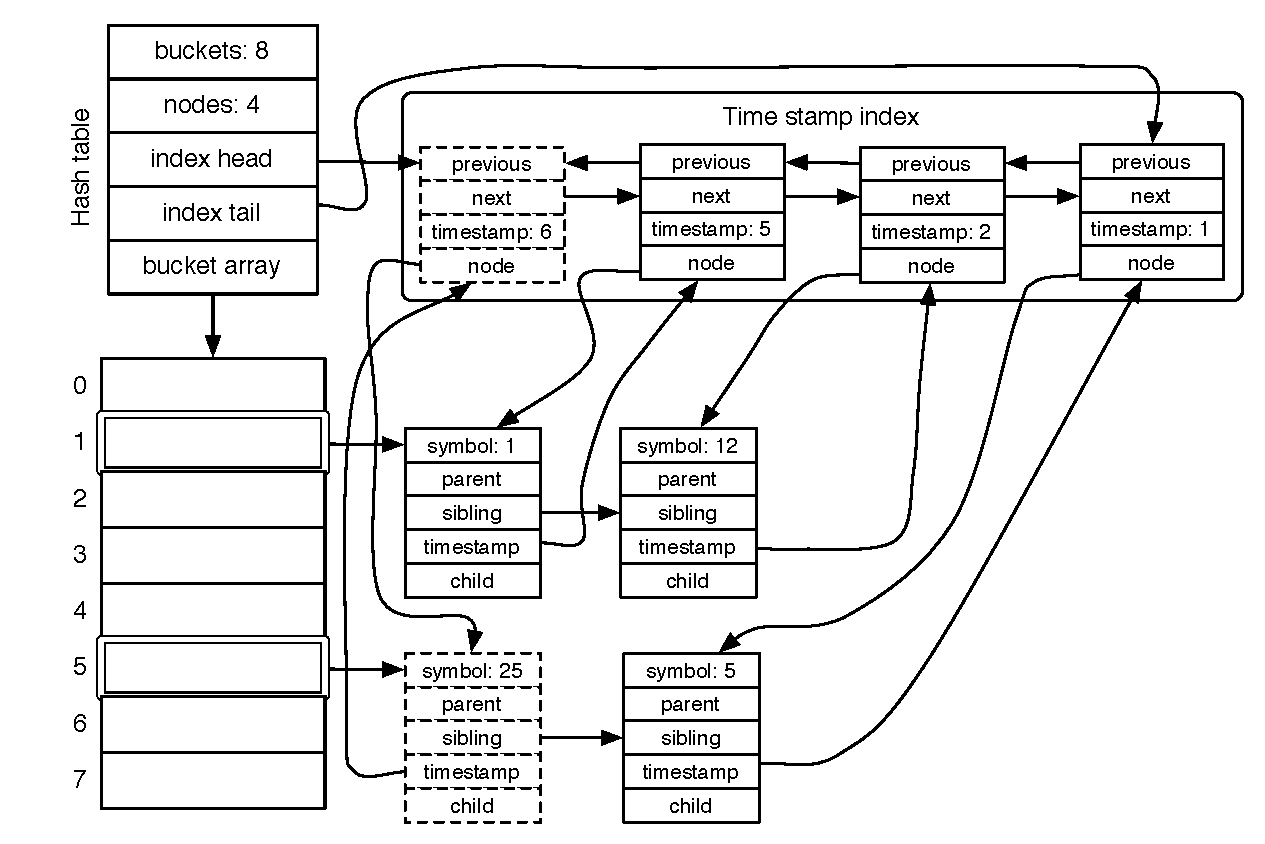
\includegraphics[scale=0.6]{hash_table_insert.pdf}
  \caption{Inserting a node into the hash table and updating the index.}
  \label{fig:hash_table_insert}
\end{figure}

\subsubsection{Updating the time stamps}

Once an answer path is inserted, the time stamps must be updated.
The new time stamp is calculated by inspecting the time stamp of the trie root node.
Next, each path node is navigated using the \texttt{parent} field until reaching the root node.

If the current node is an hashed node and the time stamp indexes
must be maintained, its index node is relocated from its position to the head of the index's double linked list. We can test wether an answer node is indexed by an hash table by inspecting
its \texttt{status} field.

Figure \ref{fig:update_timestamps} contains the pseudo-code for the function \texttt{update\_timestamps}.

\begin{figure}[ht]
\begin{Verbatim}[fontsize=\small]
update_timestamps(leaf, root, maintain_tsi) {
  new_timestamp = timestamp(root) + 1
  
  if(maintain_tsi)
    do {
      if is_hashed_node(leaf)
        // relocate index node
        promote_entry(leaf, new_timestamp)
      else
        timestamp(leaf) = new_timestamp
      leaf = parent(leaf)
    } while leaf != root
  else
    do {
      timestamp(leaf) = new_timestamp
      leaf = parent(leaf)
    } while leaf != root
  timestamp(root) = new_timestamp
}
\end{Verbatim}
\caption{Pseudo-code for \texttt{update\_timestamps}.}
\label{fig:update_timestamps}
\end{figure}

When relocating an index node $N$, the \texttt{index head} of the hash table must be modified
to point to $N$. If the $N$ was at the end of the chain,
the field \texttt{index tail} must be updated to the \texttt{previous} field of $N$.
Previous pointers of the \texttt{next} node of $N$ and the next pointer of
the \texttt{previous} node of $N$ must
also be modified to keep the chain consistent.
Figure \ref{fig:hash_table_promote} illustrates the relocation of an index node, during
the time stamp update to 7.

\begin{figure}[ht]
  \centering
    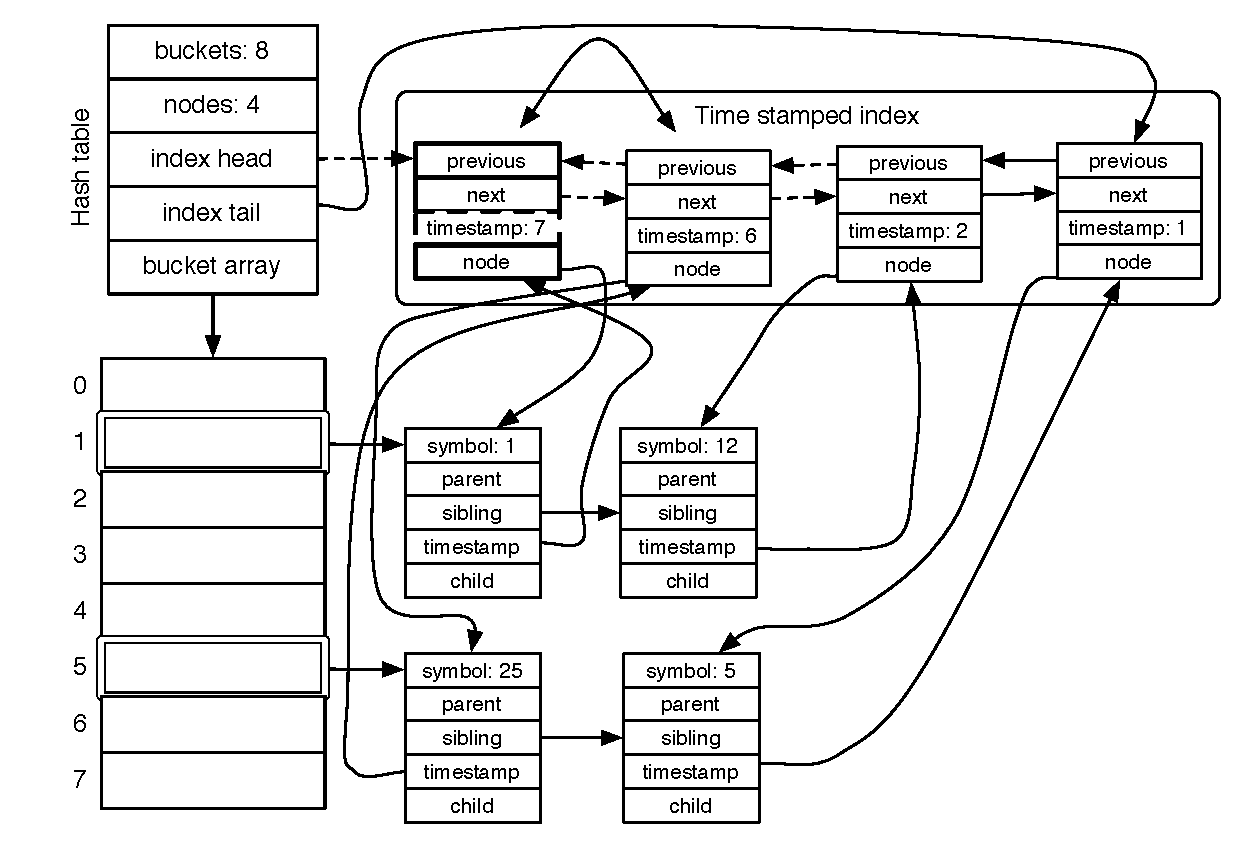
\includegraphics[scale=0.6]{hash_table_promote.pdf}
  \caption{Promoting an index node.}
  \label{fig:hash_table_promote}
\end{figure}

\subsubsection{Lazy creation of time stamp indexes}

Time stamped indexes are only maintained when consumer subgoals are first called.
When the first consumer appears, we must iterate over all the hash tables present
on the trie and create the time stamp index.

To efficiently locate all hash tables in an answer trie, we chain these hash tables
with an extra attribute named \texttt{next}. The start of this chain is stored
as the sibling node of the root answer trie node.

Creating the index for an hash table amounts to iterating over the hashed nodes
and orderly inserting new index nodes on the index chain, as it is being created.

When a subgoal completes, the time stamp indexes, which are only used
during collection of relevant answers
for consumer subgoals, are thrown away to save space.

\section{Collecting Relevant Answers}

The process of collecting relevant answers for a consumer subgoal $G$ from an answer trie $T$
of the generator subgoal $G'$, involves searching $T$ for a set $S$ of answers that unify
with the consumer answer template $AT$ and are newer than time stamp
$TS$ stored in the consumer subgoal frame.
When the process ends, $TS$ is updated to the
timestamp of the root node of $T$, thus avoiding repeated answers in future iterations
of the algorithm. Collected answers are also appended into the list of answers of the consumer subgoal frame, so they can be reused in future calls of $G$.

Various data structures are used for this algorithm, namely:

\begin{itemize}
  \item \textbf{WAM data structures}: the push down list (PDL),
  heap, trail, and associated registers. The heap is used to build complex terms, in which the
  answer template or trie variables are bound. Whenever a variable is bound, we trail it using the WAM trail. The \textit{unify} operation provided by the WAM is used to check for term equality in structured terms;
  
  \item \textbf{term stack}: used to store the next terms to be processed as we navigate through the time stamped;
  
  \item \textbf{term log stack}: when an unification fails, there is a need to backtrack to inspect other branch alternatives, this stack is used to store already processed terms of the term stack, so they can be restored back during backtracking;
  
  \item \textbf{variable bindings vector}: stores binds for trie variables;
  
  \item \textit{choice point stack}: stores choice point frames, where each frame is a search alternative and contains information to restore the state of the computation during the frame's creation.
  
\end{itemize}

The pseudo-code for the algorithm is presented in Figure \ref{fig:tst_collect_relevant_answers}.
It starts by pushing the answer template on the term stack, so that the first component to be unified is at the top. Next, we determine the base trail value by comparing TR against the trail freeze register TR\_FZ, this value can then be used to unbind variables before exiting. The trail register is set to the next free position of the WAM trail, thus avoiding writing on frozen segments. Registers HB, H and TR are saved as they will be manipulated and need to be restored to avoid any interference with the normal WAM execution. Answers gathered during execution are maintained in a linked list of trie leafs and are returned once search is over.

The whole algorithm can be summarized into seven steps:

\begin{enumerate}
  \item Fetch a term $T$ from the term stack;
  \item Search for a node $N$ at the current trie level that: (1) has a valid time stamp (2) unifies with $T$;
  \item Search for the next valid node to be pushed on the choice point stack;
  \item Unify $T$ with the trie symbol of $N$;
  \item Proceed into the child of $N$ or, if step 4 fails, backtrack by popping a frame from the choice point stack and use the alternative node to unify;
  \item Once a leaf is reached, mark a new answer and possibly backtrack to retrieve more answers and go to step (1).
  \item If no more choice point frames exist, return the marked answers.
\end{enumerate}

\begin{figure}[ht]
\begin{Verbatim}[fontsize=\small]
tst_collect_relevant_answers(trie_root, ts, answer_template)
{
  answers = new List()
  
  termstack_push_template(answer_template)
  
  // save WAM registers
  trail_base = TR > TR_FZ ? TR : TR_FZ
  saved_HB = HB
  saved_H = HB = H
  saved_TR = TR
  TR = TR > TR_FZ ? TR : TR_FZ
  
  parent = trie_root
  chain = child(parent)
  
while_loop:
  while(termstack is not empty) {
    subterm = deref(termstack_pop())
    
    if(subterm is atom or integer)
      unify_constant(subterm)
    else if(subterm is functor or list)
      unify_structured_term(subterm)
    else if(subterm is variable)
      unify_variable(subterm)
      
    if choice point stack is empty
      unwind_trail(trail_base)
      restore_wam_registers()
      return answers
    
    choice_point_backtrack()
  }
  
  // new relevant answer found
  list_insert_answer(answers, parent)
  
  // no more choice points?
  if choice point stack is empty
    unwind_trail(trail_base)
    restore_wam_registers()
    return answers
    
  choice_point_backtrack()
  goto while_loop
}
\end{Verbatim}
\caption{Pseudo-code for \texttt{tst\_collect\_relevant\_answers}.}
\label{fig:tst_collect_relevant_answers}
\end{figure}

\subsubsection{Choice Point Stack}

Each choice point frame (Figure \ref{fig:choice_point_stack}) stores the alternative node to explore, the top of the term stack, the top of the term log stack, the current trail position, and the register HB. The HB register serves the same purpose as a WAM choice point saved HB, it is used to store the value of the H register during the choice point creation, so it can restored when backtracking. Figure \ref{fig:cpstack_push_frame} presents pseudo-code for the function \texttt{cpstack\_push\_frame}, which creates a new choice point frame.

\begin{figure}[H]
  \centering
    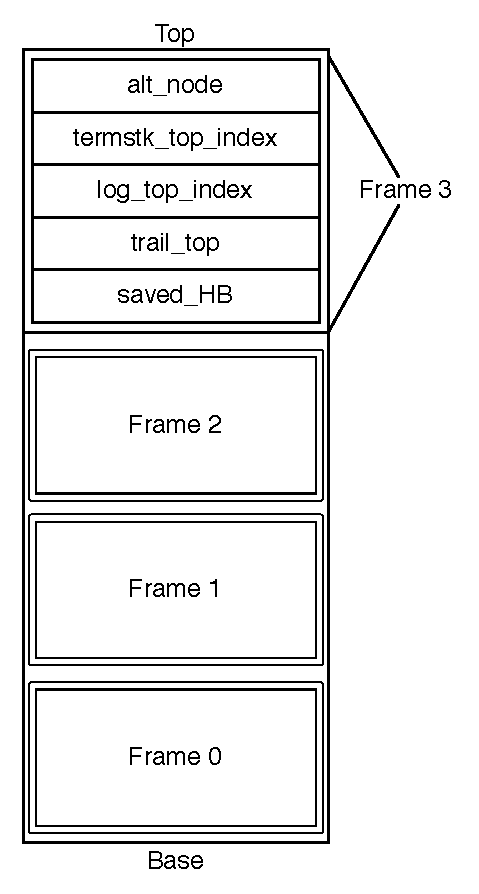
\includegraphics[scale=0.6]{choice_point_stack.pdf}
  \caption{Choice point stack organization.}
  \label{fig:choice_point_stack}
\end{figure}

During execution, the value of the WAM's HB register is compared against the value H to determine if a variable is \textit{conditional}, that is, to determine if a variable needs to be trailed, so that when execution backtracks to a previous choice point we can reset variable bindings. In our case, instead of executing WAM code, we unify a time stamped node, thus the meaning of a conditional variable is extended to include trie variables through the variable bindings vector.

\begin{figure}[H]
\begin{Verbatim}[fontsize=\small]
cpstack_push_frame(alt_node) {
  if alt_node is NULL
    return
  
  CPFrame frame = new Frame()
  frame.alt_node = alt_node
  frame.termstk_top_index = termstack_top() - termstack_base() + 1
  frame.log_top_index = termstacklog_top() - termstacklog_base()
  frame.trail_top = TR
  frame.saved_HB = H
  
  cpstack_push(frame)
}
\end{Verbatim}
\caption{Pseudo-code for \texttt{cpstack\_push\_frame}.}
\label{fig:cpstack_push_frame}
\end{figure}

When a choice point frame is popped from the stack (Figure \ref{fig:cpstack_pop_frame}),
the state of the computation is resumed:

\begin{itemize}
  \item the current node and parent node are reset;
  \item all terms stored in the term log stack are pushed into the term stack;
  \item the trail is unwinded to reset variables that existed during the choice point creation and were bound to terms;
  \item registers H and HB are also reseted to previous values.
\end{itemize}

\begin{figure}[H]
\begin{Verbatim}[fontsize=\small]
cpstack_pop_frame() {
  Frame top_frame = cpstack_pop()
  
  chain = top_frame.alt_node
  parent = parent(chain)
  termstacklog_unwind(top_frame.log_top_index)
  termstack_set_top_of_stack(top_frame.termstk_top_index)
  trail_unwind(top_frame.trail_top)
  H = HB
  HB = top_frame.saved_HB
}
\end{Verbatim}
\caption{Pseudo-code for \texttt{cpstack\_pop\_frame}.}
\label{fig:cpstack_pop_frame}
\end{figure}

\subsubsection{Unify with constant}

Once a trie node $N$ is reached we must select the next trie node $N'$ that unifies with our term and has a valid time stamp. Node $N$ can lead either to a simple node chain or an hash table.
With constant terms we can index the hash table to prune the search space (\texttt{set\_match\_and\_unify\_chains}) by using the \textit{match bucket}.

\begin{figure}[H]
\begin{Verbatim}[fontsize=\small]
unify_constant(constant) {
  if is_hash_table(chain)
    // retrieve the indexed and variable buckets
    (chain, alt_chain) = set_match_and_unify_chains(constant)
    if chain != alt_chain
      search_chain_exact_match(chain, constant, ts, alt_chain)
      // exact match failed
      chain = alt_chain
    if chain is NULL
      backtrack
  search_chain_unify_with_constant(chain, constant, ts)
}
\end{Verbatim}
\caption{Pseudo-code for \texttt{unify\_constant}.}
\label{fig:unify_constant}
\end{figure}

Because variables can unify with the constant term, there is the need to retrieve the variable chain (from the variable bucket), which will be used as the alternative chain to push on the choice point stack. We call it the \textit{unify chain}. If the constant is found on the match chain, the unify chain is used as alternative, but if no match was found, the variable chain will be attempted next and, depending on the remaining nodes, also be used as the backtracking alternative.

\begin{figure}[H]
\begin{Verbatim}[fontsize=\small]
search_chain_exact_match(chain, term, ts, alt_chain) {
  foreach(node in chain) {
    if(term == symbol(node))
      if(valid_timestamp(timestamp(node), ts))
        cpstack_push_frame(chain_next_valid_node(alt_chain, ts))
        termstacklog_push(termstack_index(), termstack_top())
        descend_tst(node)
      else
        return NULL
  }
  return NULL
}
\end{Verbatim}
\caption{Pseudo-code for \texttt{search\_chain\_exact\_match}.}
\label{fig:search_chain_exact_match}
\end{figure}

In Figure \ref{fig:unify_constant} we present the pseudo-code for \texttt{unify\_constant}. Note that we check for an hash table first and inspect the match bucket using \texttt{search\_chain\_exact\_match} (Figure \ref{fig:search_chain_exact_match}).
Finally, if no match is found we set \texttt{chain} to \texttt{alt\_chain} (the unify chain) and execute \texttt{search\_chain\_unify\_with\_constant} on the unify chain. If no hash table was found, we would consider the simple chain of sibling nodes as the unify chain and simply execute \texttt{search\_chain\_unify\_with\_constant}.

\begin{figure}[H]
\begin{Verbatim}[fontsize=\small]
search_chain_unify_with_constant(chain, constant, ts) {
  chain = chain_next_valid_node(chain, ts)
  while(chain is not null) {
    alt_chain = chain_next_valid_node(sibling(chain), ts)
    symbol = trie_deref(symbol(chain))
    if symbol is variable // case (1)
      cpstack_push_frame(alt_chain)
      bind_and_conditionally_trail(symbol, constant)
      termstacklog_push(constant)
      descend_tst(chain)
    else if symbol == constant // case (2)
      // exact match
      cpstack_push_frame(alt_chain)
      termstacklog_push(constant)
      descend_tst(node)
    else
      chain = alt_chain
  }
  // case (3)
}
\end{Verbatim}
\caption{Pseudo-code for \texttt{search\_chain\_unify\_with\_constant}.}
\label{fig:search_chain_unify_with_constant}
\end{figure}

When using a unify chain, we locate the next node with a valid time stamp on the chain, that is, with the time stamp greater than our target time stamp. Next we "dereference" the node symbol by using
\texttt{trie\_deref}, which returns a position on the variable bindings vector if the node symbol is a trie variable, hence allowing trie variables to be used as "normal" variables.

Please note that the function \texttt{bind\_and\_conditionally\_trail} tests if the variable (first argument) is a conditional variable and then trails it using the WAM trail.

In case (1), a variable was found, which can be a position on the variable bindings vector or a prolog variable that was bound to a trie variable; either way, we bind the variable to the constant term, push a new choice point frame with the next valid node, and descend into the child node of \texttt{chain}.

In case (2) the node symbol matches our constant and we simply push a new choice point frame and advance into the next node.

If we could not found a valid trie node in the unify chain, case (3), the next choice point is popped from the choice point stack and the alternative is tried. If the stack is empty, the algorithm finally ends.

As an example, let's consider the time stamped trie in Figure \ref{fig:collect_example_1}. The input answer template is $\{$\texttt{a,b,b}$\}$ and the target time stamp is 3.

\begin{figure}[H]
  \centering
    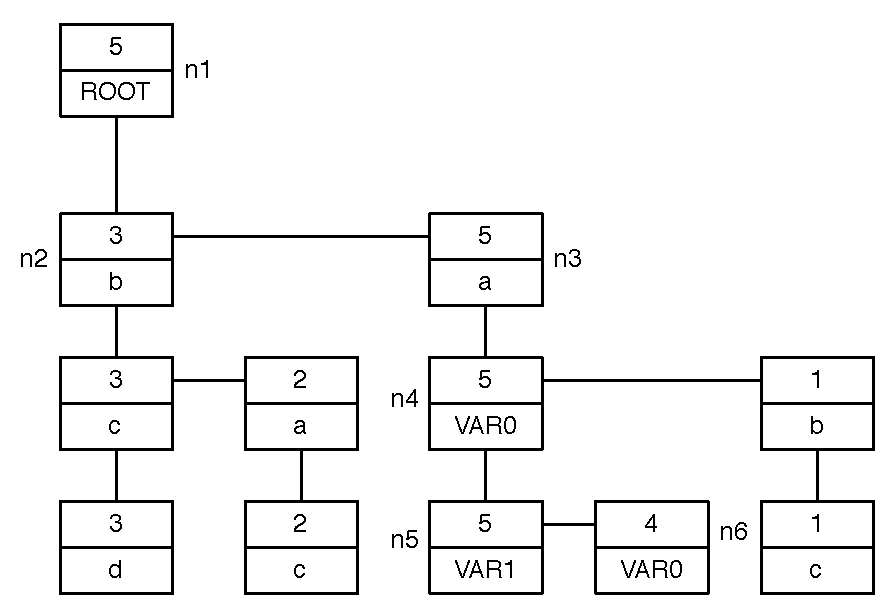
\includegraphics[scale=0.6]{collect_example_1.pdf}
  \caption{Example time stamped trie.}
  \label{fig:collect_example_1}
\end{figure}

We start on node (a) (Figure \ref{fig:collect_ex1}), the root of the trie. The unify chain
is composed by nodes (b) and (c). Node (b) is discarded because the time stamp is invalid.
Node (c) has a valid time stamp and its symbol matches with the current term, \texttt{a}.

\begin{figure}[H]
  \centering
    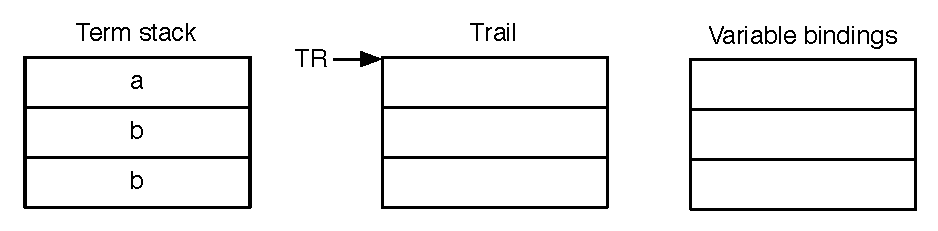
\includegraphics[scale=0.6]{collect_ex1.pdf}
  \caption{At trie node (a).}
  \label{fig:collect_ex1}
\end{figure}

On node (c), our first alternative, node (d) has a valid time stamp and, after doing
\texttt{trie\_deref} we find an unbound variable, \textbf{VAR0}, which is represented
by the first position of the variable bindings vector.
This variable is trailed and bound to \texttt{b},
resulting in what is presented in Figure \ref{fig:collect_ex2}.

\begin{figure}[H]
  \centering
    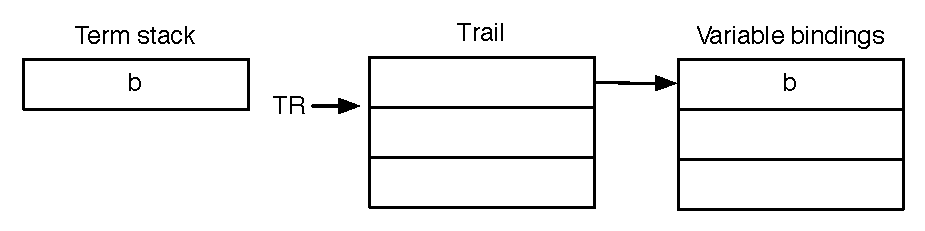
\includegraphics[scale=0.6]{collect_ex2.pdf}
  \caption{At trie node (d).}
  \label{fig:collect_ex2}
\end{figure}

On node (d), the unify chain is composed by nodes (e) and (f). Both have valid time stamps (> 3).
Node (e) is attempted first and easily unifies, because it is an unbound trie variable.
Leaf node (e) is our first answer (Figure \ref{fig:collect_ex3}).

\begin{figure}[H]
  \centering
    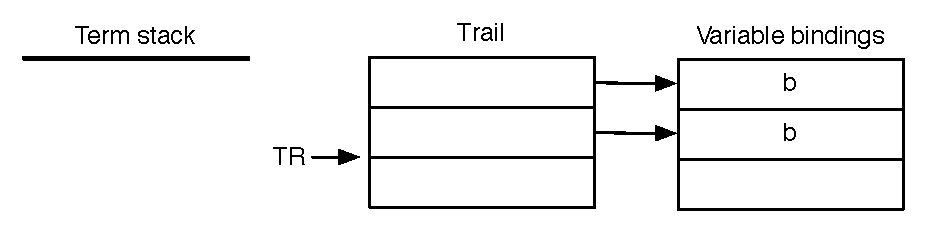
\includegraphics[scale=0.6]{collect_ex3.pdf}
  \caption{At trie node (e).}
  \label{fig:collect_ex3}
\end{figure}

Now, we need to backtrack to collect the other answers. The top choice point frame is retrieved from the stack resulting in a variable being untrailed and the term \texttt{b} being pushed into the term stack (Figure \ref{fig:collect_ex4}).

\begin{figure}[H]
  \centering
    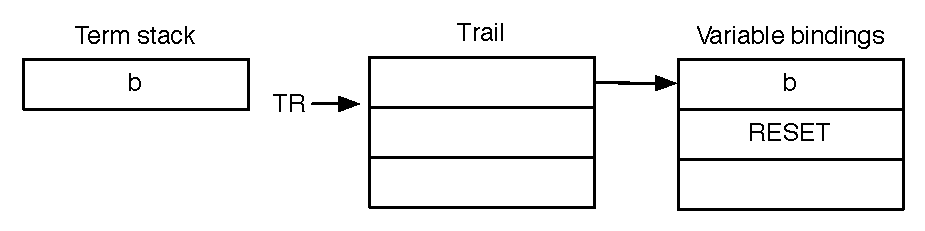
\includegraphics[scale=0.6]{collect_ex4.pdf}
  \caption{Backtracking to node (f).}
  \label{fig:collect_ex4}
\end{figure}

In node (f) we dereference the trie variable \texttt{VAR0} and get the constant term \texttt{b}, which matches the target term. No binding or trailing is needed and we succeed in collecting another relevant answer (Figure \ref{fig:collect_ex5}).

\begin{figure}[H]
  \centering
    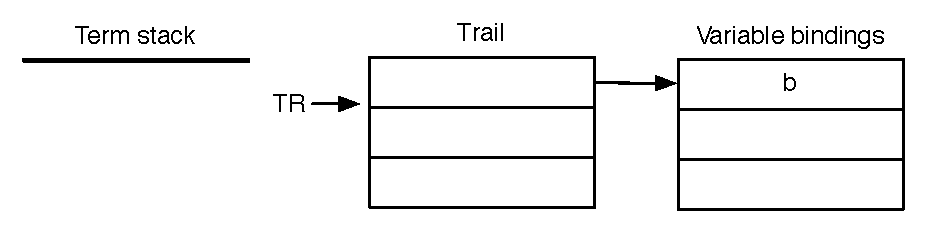
\includegraphics[scale=0.6]{collect_ex5.pdf}
  \caption{New answer as the leaf node (f).}
  \label{fig:collect_ex5}
\end{figure}

As there are no more available choice points we need to untrail any bindings made and return
the answers found (Figure \ref{fig:collect_ex6}), finishing the search.

\begin{figure}[H]
  \centering
    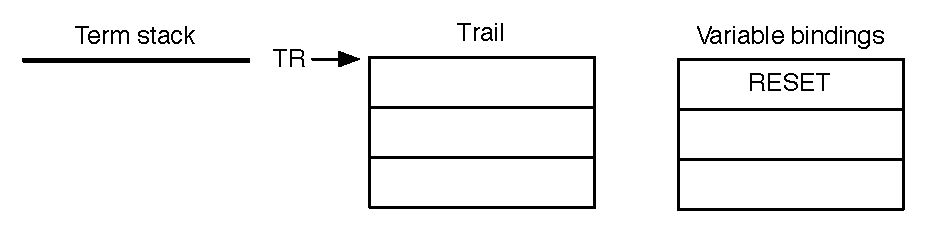
\includegraphics[scale=0.6]{collect_ex6.pdf}
  \caption{Untrailing variables and returning.}
  \label{fig:collect_ex6}
\end{figure}

\subsubsection{Unify with structured term}

For structured terms, the unification process is similar to constant unification. The
current term in the term stack must be a functor or a list. First, we check if the current
trie node is an hash table and the match and unify chains are computed.
If the match chain contains a valid trie node, before we descend into the child
node we must push the functor or list arguments into the term stack, so they can
be unified with the next trie nodes.

\begin{figure}[H]
\begin{Verbatim}[fontsize=\small]
unify_structured_term(term) {
  if is_hash_table(chain)
    // retrieve the indexed and variable buckets
    (chain, alt_chain) = set_match_and_unify_chains(term)
    if chain != alt_chain
      search_chain_exact_match_push(chain, term, ts, alt_chain)
      // exact match failed
      chain = alt_chain
    if chain is NULL
      backtrack
  search_chain_unify_with_structured_term(chain, term, ts)
}
\end{Verbatim}
\caption{Pseudo-code for \texttt{unify\_structured\_term}.}
\label{fig:unify_structured_term}
\end{figure}

When using the unify chain with \texttt{search\_chain\_unify\_with\_structured\_term}
\ref{fig:search_chain_unify_with_structured_term},
we also loop the chain for valid time stamped nodes.
Four situations may arise:

\begin{enumerate}
  \item The current term is variable, which is trail and bound to the structured term;
  \item The trie symbol is a structured term and matches our functor or list.
  The term arguments are pushed into the term stack for unification;
  \item We find a trie variable bound to a structured term. The WAM function \texttt{unify} is executed to check for a match and perform additional unifications;
  \item No match was found, the next alternative node is inspected.
\end{enumerate}

\begin{figure}[H]
\begin{Verbatim}[fontsize=\small]
search_chain_unify_with_structured_term(chain, term, ts) {
  chain = chain_next_valid_node(chain, ts)
  while(chain is not null) {
    alt_chain = chain_next_valid_node(sibling(chain), ts)
    symbol = trie_deref(symbol(chain))
    if symbol is variable // case (1)
      cpstack_push_frame(alt_chain)
      bind_and_conditionally_trail(symbol, term)
      termstacklog_push(term)
      descend_tst(chain)
    else if symbol is a structured term
      if original type of symbol is a structured term and symbol == term
        // case (2)
        cpstack_push_frame(alt_chain)
        termstacklog_push(term)
        termstack_push_arguments(term)
        descend_tst(chain)
      else if unify(term, symbol) // case (3)
        // trie variable bound to an heap structured term
        cpstack_push_frame(alt_chain)
        termstacklog_push(term)
        descend_tst(node)
    else
      chain = alt_chain
  }
  // case (4)
}
\end{Verbatim}
\caption{Pseudo-code for \texttt{search\_chain\_unify\_with\_structured\_term}.}
\label{fig:search_chain_unify_with_structured_term}
\end{figure}

Let's consider the time stamped trie in Figure \ref{fig:collect_functor}
and the following answer template: $\{$\texttt{STR 3, STR 6, STR 9}$\}$.
The target time stamp is 1.

\begin{figure}[H]
  \centering
    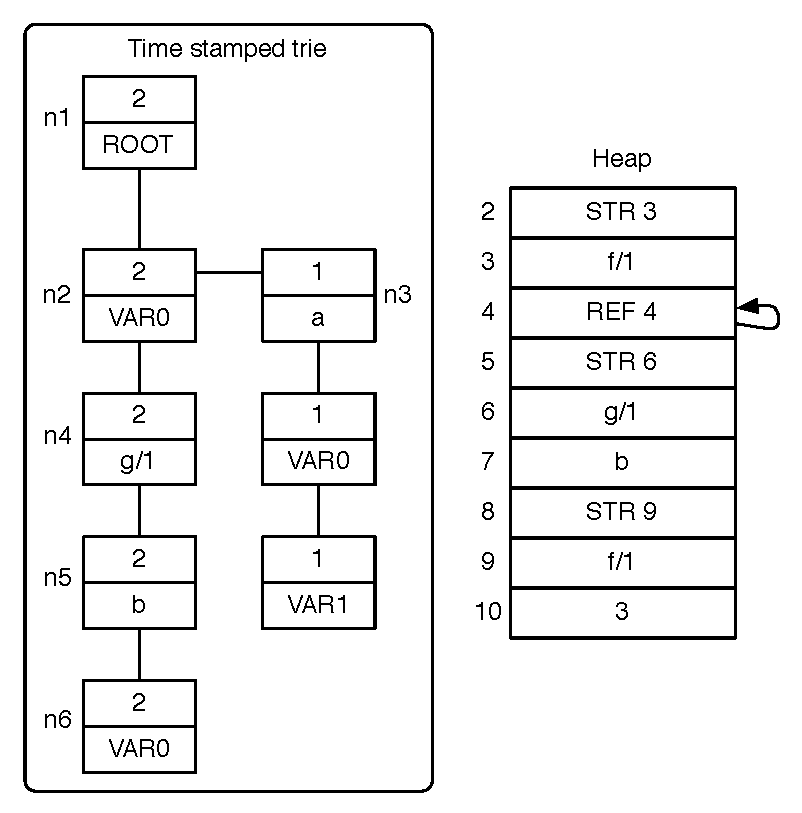
\includegraphics[scale=0.6]{collect_functor.pdf}
  \caption{Example time stamped trie and heap with terms referenced in the answer template.}
  \label{fig:collect_functor}
\end{figure}

At node (a) the term stack contains the full answer template and the variable bindings vector
is empty \ref{fig:collect_functor1}. Only node (b) satisfies the time stamp requirements,
as $2 > 1$.

\begin{figure}[H]
  \centering
    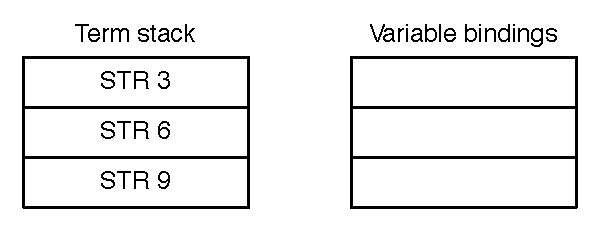
\includegraphics[scale=0.6]{collect_functor1.pdf}
  \caption{Term stack and variable bindings vector at node (a).}
  \label{fig:collect_functor1}
\end{figure}

Node (b) contains a trie variable and the current term is \texttt{STR 3} or \texttt{f(VAR)}.
In this situation, the variable bindings position for \textbf{VAR0} is trailed and bound to \texttt{STR 3}. The data structures configuration is presented in Figure \ref{fig:collect_functor2}.

\begin{figure}[H]
  \centering
    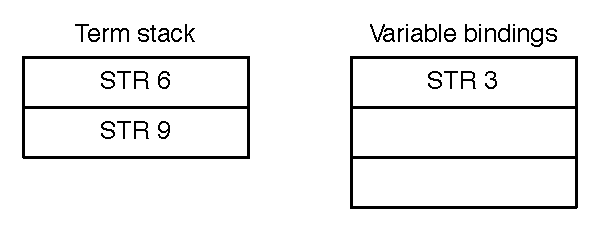
\includegraphics[scale=0.6]{collect_functor2.pdf}
  \caption{Term stack and variable bindings vector at node (b).}
  \label{fig:collect_functor2}
\end{figure}

Node (d) contains the symbol \texttt{g/1} and the current term is \texttt{STR 6}
or \texttt{g(b)}, which matches. The argument \texttt{b} of \texttt{g(b)}
is pushed into the term stack to be processed in the next node (Figure \ref{fig:collect_functor3}).

\begin{figure}[H]
  \centering
    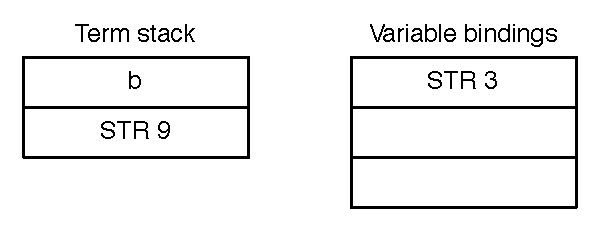
\includegraphics[scale=0.6]{collect_functor3.pdf}
  \caption{Term stack and variable bindings vector at node (d).}
  \label{fig:collect_functor3}
\end{figure}

Node (e) has the symbol \texttt{b} which matches with \texttt{b} from the term stack and
execution proceeds to node (f) (Figure \ref{fig:collect_functor4}).

\begin{figure}[H]
  \centering
    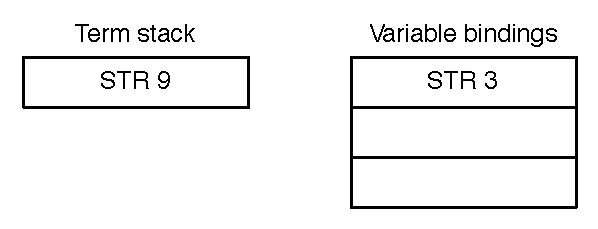
\includegraphics[scale=0.6]{collect_functor4.pdf}
  \caption{Term stack and variable bindings vector at node (e).}
  \label{fig:collect_functor4}
\end{figure}

At (f) we find a trie variable, which, after being dereferenced, contains the
functor \texttt{f(VAR)}. The current term to be unified is \texttt{f(3)}.
In this situation we call \texttt{unify}, which will try to unify both terms.
The unification has the side effect of setting the heap variable cell 4 to \texttt{3}
(Figure \ref{fig:collect_functor5}).
This variable is conditional because it is positioned before the register \texttt{HB},
which given the algorithm design must be greater than 10.

\begin{figure}[H]
  \centering
    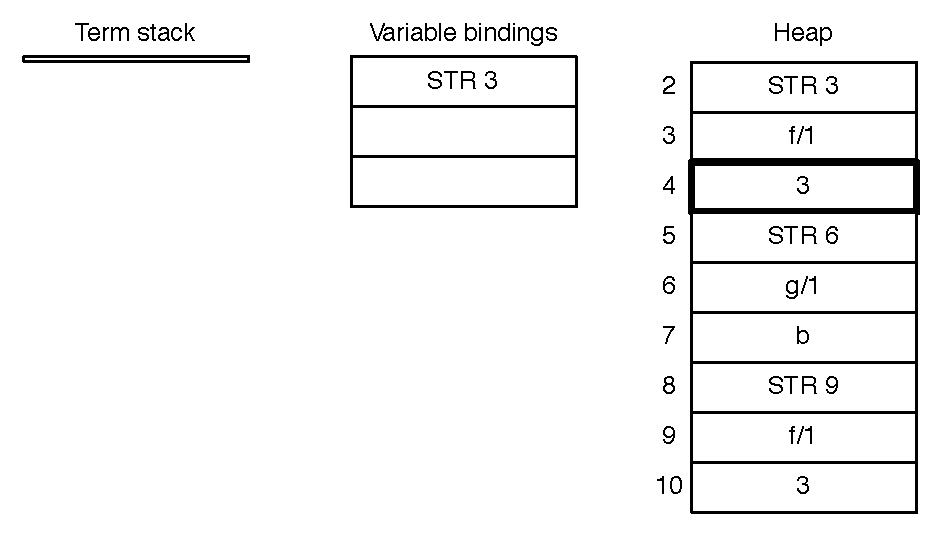
\includegraphics[scale=0.6]{collect_functor5.pdf}
  \caption{Term stack, variable bindings vector and heap at node (f).}
  \label{fig:collect_functor5}
\end{figure}

\subsubsection{Unify with variable}

Because variables unify with anything, when the top of the term
stack is a variable, the next trie branches only need to be pruned using the time stamp.

Figure \ref{fig:unify_variable} presents the function
\texttt{unify\_variable}. Here, we have three cases:

\begin{enumerate}
  \item The current chain link is an hash table. In this situation we can select the next transitions by using the time stamped index, which can easily prune based on the time stamp;
  \item The current node is inside an hash table, thus is on the time stamped index. The node is matched against the variable and the alternative node is selected by following the index chain links;
  \item Current node is a simple sibling chain. Both the chain and the alternative chain are set by iterating over the node chain, looking for valid time stamps.
\end{enumerate}

Once chains are set, we create a new choice point, run the variable unification algorithm
and proceed into the next trie node.

\begin{figure}[H]
\begin{Verbatim}[fontsize=\small]
unify_variable(var) {
  if is_hash_table(chain) // case (1)
    index = index_head(chain)
    if timestamp(index) > ts
      chain = node(index)
      alt_chain = next_valid_index(index, ts)
    else backtrack
  else if is_hashed_node(chain) // case (2)
    // can only be here via backtracking
    alt_chain = next_valid_index(get_index(chain), ts)
  else // case (3)
    // simple chain of siblings
    chain = chain_next_valid_node(chain, ts)
    if chain is NULL backtrack
    alt_chain = sibling(chain)
  
  cpstack_push_frame(alt_chain)
  termstacklog_push(var)
  symbol = trie_deref(symbol(chain))
  unifiy_with_variable(var, symbol, chain)
  descend_tst(chain)
}
\end{Verbatim}
\caption{Pseudo-code for \texttt{unify\_variable}.}
\label{fig:unify_variable}
\end{figure}

From the pseudo-code in Figure \ref{fig:unify_with_variable}, variable unification
must consider the following situations:

\begin{itemize}
  \item symbol is a constant: the term variable is bound to the symbol and conditionally trailed.
  \item symbol is a structured term: if the symbol was a trie variable bound to a term then we bind the variable to the heap location; else, we create a new structure (functor or list) on the heap and bind the variable to it, resulting in a term with various heap variables as arguments, which will be pushed into the term stack and will be bound in the next iterations of the algorithm.
  \item symbol is a variable: if the variable is a trie variable, we bind and trail it; if it is an heap variable that was dereferenced from a trie variable using \texttt{trie\_deref}, \texttt{unify} chooses the binding direction, resulting in one of the variables being trailed.
\end{itemize}

\begin{figure}[H]
\begin{Verbatim}[fontsize=\small]
unify_with_variable(var, symbol, node) {
  if symbol is a constant
    bind_and_conditionally_trail(var, symbol)
  else if symbol is a structured term
    if node symbol is a structured term
      bind_and_conditionally_trail(var, H)
      create_heap_structure(symbol)
      termstack_push_arguments(deref(var))
    else
      // trie variable bound to an heap structure
      bind_and_conditionally_trail(var, symbol)
  else if symbol is a variable
    if symbol is a trie variable
      bind_and_trail(symbol, var)
    else
      // two heap variables
      unify(symbol, var)
  else
    backtrack
}
\end{Verbatim}
\caption{Pseudo-code for \texttt{unify\_with\_variable}.}
\label{fig:unify_with_variable}
\end{figure}

As an example, consider the trie and heap in Figure \ref{fig:collect_variable}.
The input answer template is $\{$\texttt{REF2,REF2,b}$\}$ and the start time stamp is 2.

\begin{figure}[H]
  \centering
    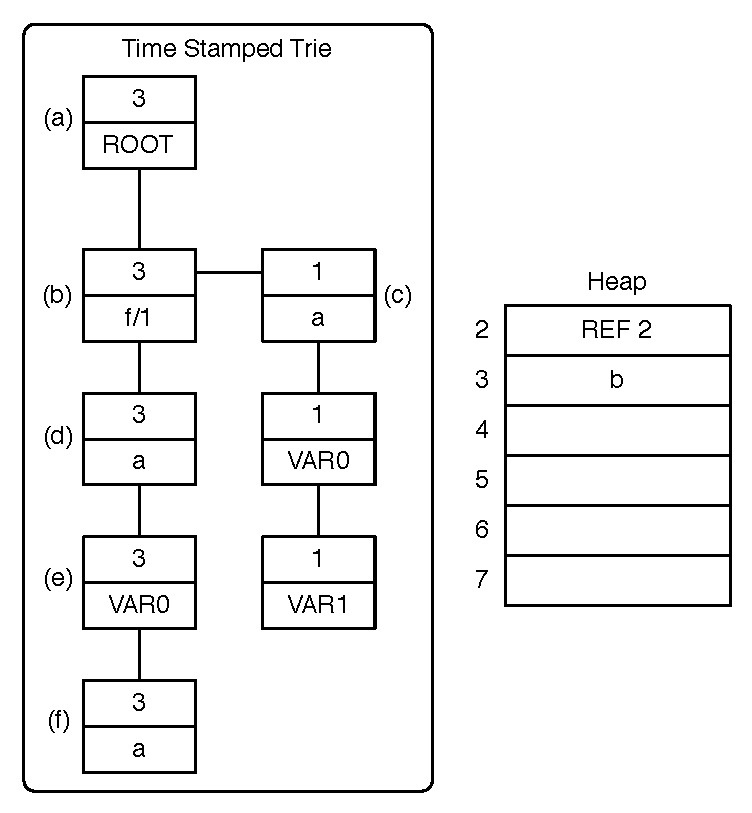
\includegraphics[scale=0.6]{collect_variable.pdf}
  \caption{Example time stamped trie and heap.}
  \label{fig:collect_variable}
\end{figure}

Starting on root node (a), we have the following data structure configuration:

\begin{figure}[H]
  \centering
    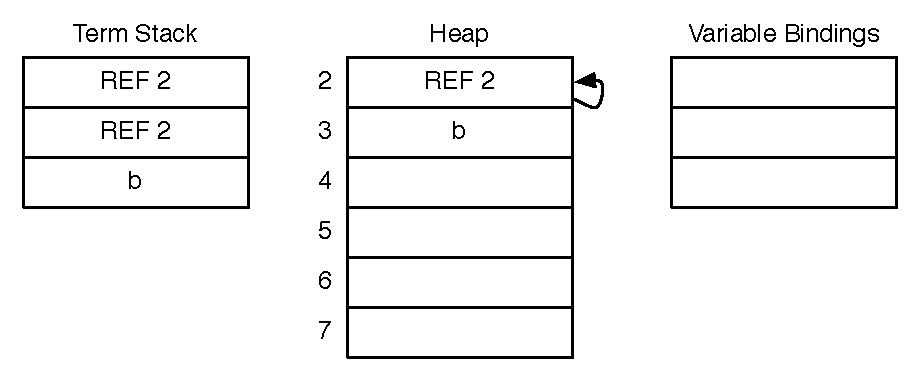
\includegraphics[scale=0.6]{collect_variable1.pdf}
  \caption{At node (a).}
  \label{fig:collect_variable1}
\end{figure}

Node (b) is the only valid transition, with time stamp 3.
The functor \texttt{f/1} is unified against the variable \texttt{REF 2},
which results in the functor \texttt{f/1} being created on the heap
and its argument (\texttt{REF 5}) being pushed into the term stack
(Figure \ref{fig:collect_variable2}).

\begin{figure}[H]
  \centering
    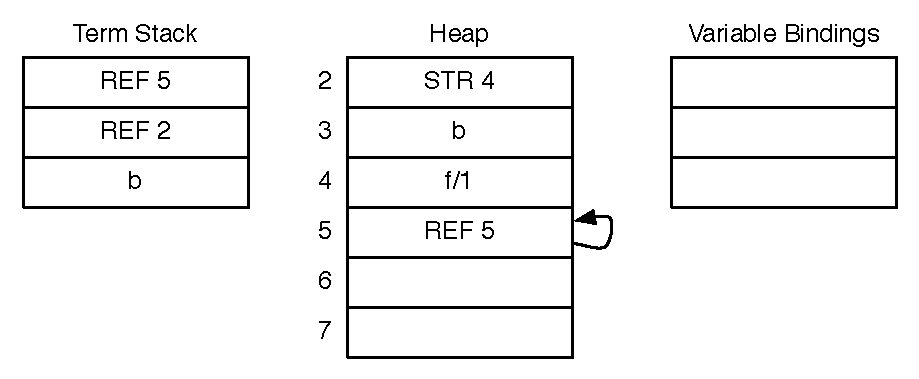
\includegraphics[scale=0.6]{collect_variable2.pdf}
  \caption{After unifying with node (b).}
  \label{fig:collect_variable2}
\end{figure}

The yet unbound functor argument matches atom \texttt{a} in node (d),
resulting in the update of the heap cell 5 (Figure \ref{fig:collect_variable3}).

\begin{figure}[H]
  \centering
    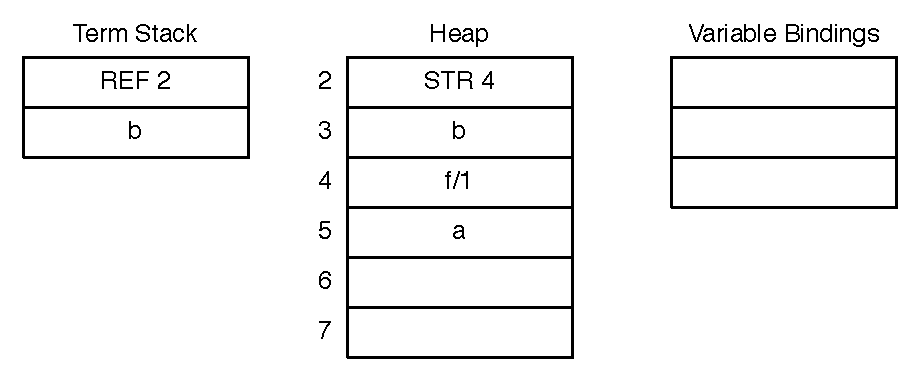
\includegraphics[scale=0.6]{collect_variable3.pdf}
  \caption{After unifying with node (d).}
  \label{fig:collect_variable3}
\end{figure}

Now on the term stack we have \texttt{REF 2}, which dereferences to
a structure on cell 4. On node (e) we have the unbound trie variable
\texttt{VAR0}, which gets bound to \texttt{STR 4} (Figure \ref{fig:collect_variable4}).

\begin{figure}[H]
  \centering
    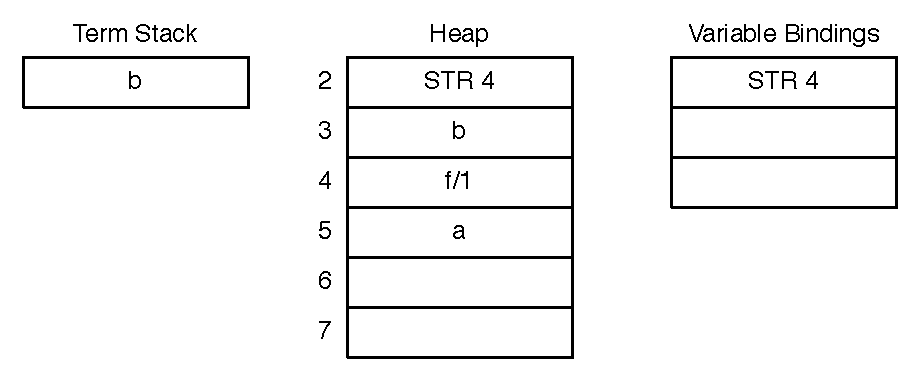
\includegraphics[scale=0.6]{collect_variable4.pdf}
  \caption{After unifying with node (e).}
  \label{fig:collect_variable4}
\end{figure}

Finally, the last term on the term stack is \texttt{b}, which
can not be matched against \texttt{a} on node (f), hence no
relevant answers are found on this trie.

\section{Consuming Answers}

Each consumer subgoal frame stores a linked list with answers that are collected
during evaluation. This list is built incrementally as new answers are generated
for the generator subgoal, which updates the generator time stamp.
Whenever a consumer choice point exhausts the answer list, the retrieval
of relevant answers is attempted so the subgoal frame answer list can be extended.

While the collection of specific answers is done by searching the answer trie
and pruning branches by time stamp and unification failure, it is all done in one
phase. The consumption of a set of answers $S$ is done by consuming one answer $A \in S$
at a time and is completely separated from the collection phase.

Assume we have a trie path from the leaf node $L$ representative of $A$ and
the trie root $R$. Consuming $A$ amounts to unify the symbols on the trie path from $R$ to $L$
to the answer template $AT$ that is built for the consumer choice point. In the end, the variables
on $AT$ are updated so the WAM evaluation branch can proceed with new bindings.

\begin{figure}[H]
  \centering
    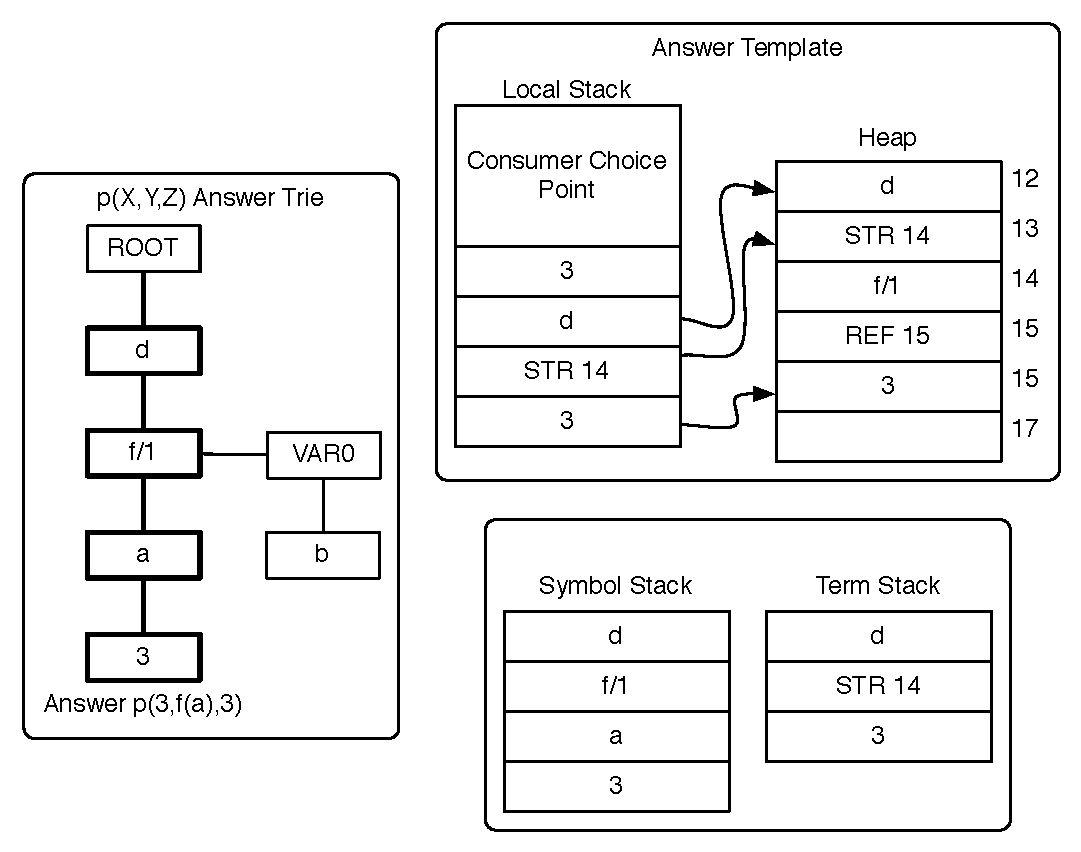
\includegraphics[scale=0.6]{consume_answer.pdf}
  \caption{Data structures related to answer consumption.}
  \label{fig:consume_answer}
\end{figure}

As we are certain that $A$ unifies with $AT$, consumption can be reduced to locating a relevant
answer in a trie with only the answer $A$, no time stamp pruning or backtracking is done.
Implementation wise, we use the term stack that is initially pushed with $AT$
and a symbol stack containing symbols from $R$ to $L$. Then, we proceed by
iteratively popping one term from the term stack and one symbol from the symbol stack
and unifying one against the other.

In Figure \ref{fig:consume_answer} we present the data structures involved in consuming
a subsumptive answer. The subsumptive subgoal is \texttt{p(X,Y,Z)} and the
subsumed subgoal is \texttt{p(d,p(X),3)}. The answer to consume is \texttt{p(d,f(a),3)}.
After the answer is consumed, the subsumed subgoal gets a new answer: \texttt{X = a}.

\section{Compiled Tries}

\section{Subsumptive YapTab}

\section{Results}




\newpage
\thispagestyle{plain}
\mbox{}

\chapter{Retroactive Call Subsumption}
This chapter explores the concept of retroactive call subsumption (RCS). RCS
enables full sharing of answers among subgoal calls, independent of the order they are called,
using the relation of subsumption.

First, we introduce the motivations behind RCS by illustrating the shortcomings of traditional call
subsumption mechanisms. Next, we present the concepts introduced by RCS and how execution
rules are extended to support retroactive tabling. Other extensions are then discussed, namely:
the new table space organization based around the ideas of the \textit{common global trie} proposal
\cite{CostaJ-08} and the algorithm to traverse the call trie to search for subsumed subgoals. Finally, we
give some details about the implementation of this new extension in the YapTab system.

\section{Motivation}

In traditional call subsumption, a new call to the subgoal $G$ is considered to create a producer subgoal
when a more general subgoal $G'$ is not found on the call trie and it is the first time $G$ is called.
When $G'$ exists, a new consumer is stored to consume answers from the subsuming subgoal $G'$, thus creating
a consumer subgoal.

Consider that subgoal \texttt{p(X,1,2)} is called first, followed by \texttt{p(X,1,Z)}.
Notice that when \texttt{p(X,1,2)} is called it is considered a producer subgoal as no subsuming subgoals
are found on the call trie. The subgoal \texttt{p(X,1,Z)} is also considered as a producer, because
\texttt{p(X,1,2)} does not subsume \texttt{p(X,1,Z)}. If the call order is swapped, \texttt{p(X,1,Z)} continues
to be considered a producer subgoal, but now \texttt{p(X,1,2)} finds \texttt{p(X,1,Z)} as a subsuming subgoal
on the call trie, and thus is considered a consumer subgoal.

While call subsumption provides good results in terms of memory utilization and time it suffers from a
major problem: the order in which the the subgoals are called can greatly affect the performance
and applicability of the technique. Therefore, we introduce a new mechanism called \textit{retroactive call
subsumption} (RCS) that solves the problem by retroactively modifying active tabled nodes to enable full sharing
of answers between subsuming and subsumed subgoals, independently of the order they are called.

\section{General Idea}

Retroactive Call Subsumption is based around the idea of stopping the computation of subsumed subgoals
that are currently running by transforming those producer subgoals into consumer subgoals, thus instead
of generating their own answers by means of code execution, they will consume answers from the more general
subgoal that has been called.

When the producer subgoal $G$ executes, an arbitrary number of choice points are created that are directly related
to $G$, that is, they are used to compute $G$'s answers. Therefore, when $G$
must be transformed into a consumer subgoal we must \textit{selectively prune} the parts of the computation
that are related to $G$ and transform $G$'s generator choice point in such a way that the choice point
will consume answers from the producer subgoal $G'$, instead of generating its own answers.
Pruning the computation of $G$ can thus potentially save execution time as $G$ no longer properly executes
but consumes answers from another subgoal.

Consider the program in Figure~\ref{fig:retro_program1} that uses RCS and the query goal `\texttt{a(X),~p(Y,Z)}'.
The goal \texttt{a(X)} starts by calling \texttt{p(1,X)}, which succeeds with the answer \texttt{\{X~=~3\}}.
By forward execution, \texttt{p(Y,Z)} is called and verifies if any subsumed subgoal is currently running
and needs to be pruned (Figure \ref{fig:retro_eval1}~(a)). It finds \texttt{p(1,X)} and thus it marks this subgoal frame as a consumer subgoal
frame that will consume from \texttt{p(Y,Z)}.
In order for \texttt{p(1,X)} to act as a consumer, its generator choice point is transformed into
a \textit{retroactive choice point}, which amounts to update the \textit{continuation alternative}
(\texttt{CP\_AP} choice point field) to an instruction called \textit{retroactive\_resolution},
which implements the needed mechanisms to control the evaluation of a \textit{retroactive node}
(Figure \ref{fig:retro_eval1}~(b)).

\begin{figure}[ht]
\begin{Verbatim}
:- use_retroactive_tabling p/2.

a(X) :- p(1, X).

p(1, 3).
p(2, 3).
p(1, 2).
\end{Verbatim}
\caption{Example program using retroactive tabling.}
\label{fig:retro_program1}
\end{figure}

Next, \texttt{p(Y,Z)} continues execution and a new answer is generated, \texttt{\{Y~=~1,~Z~=~3\}}.
By means of backtracking, all answers for \texttt{p(Y,Z)} are generated and the subgoal finally completes.
Execution returns to the retroactive choice point of \texttt{p(1,X)} and retroactive resolution is employed.
As the producer subgoal, \texttt{p(Y,Z)} has already completed, \texttt{p(1,X)} can be turned into a loader
node to consume all answers relevant to the subgoal that were not generated when the subgoal was a generator.
In this case, the only answer available is \texttt{\{X~=~2\}} (Figure \ref{fig:retro_eval1}~(c)).
Note that a retroactive node can be transformed into other types of nodes, as it will become clear in the next
sections.

\begin{figure}[ht]
  \centering
    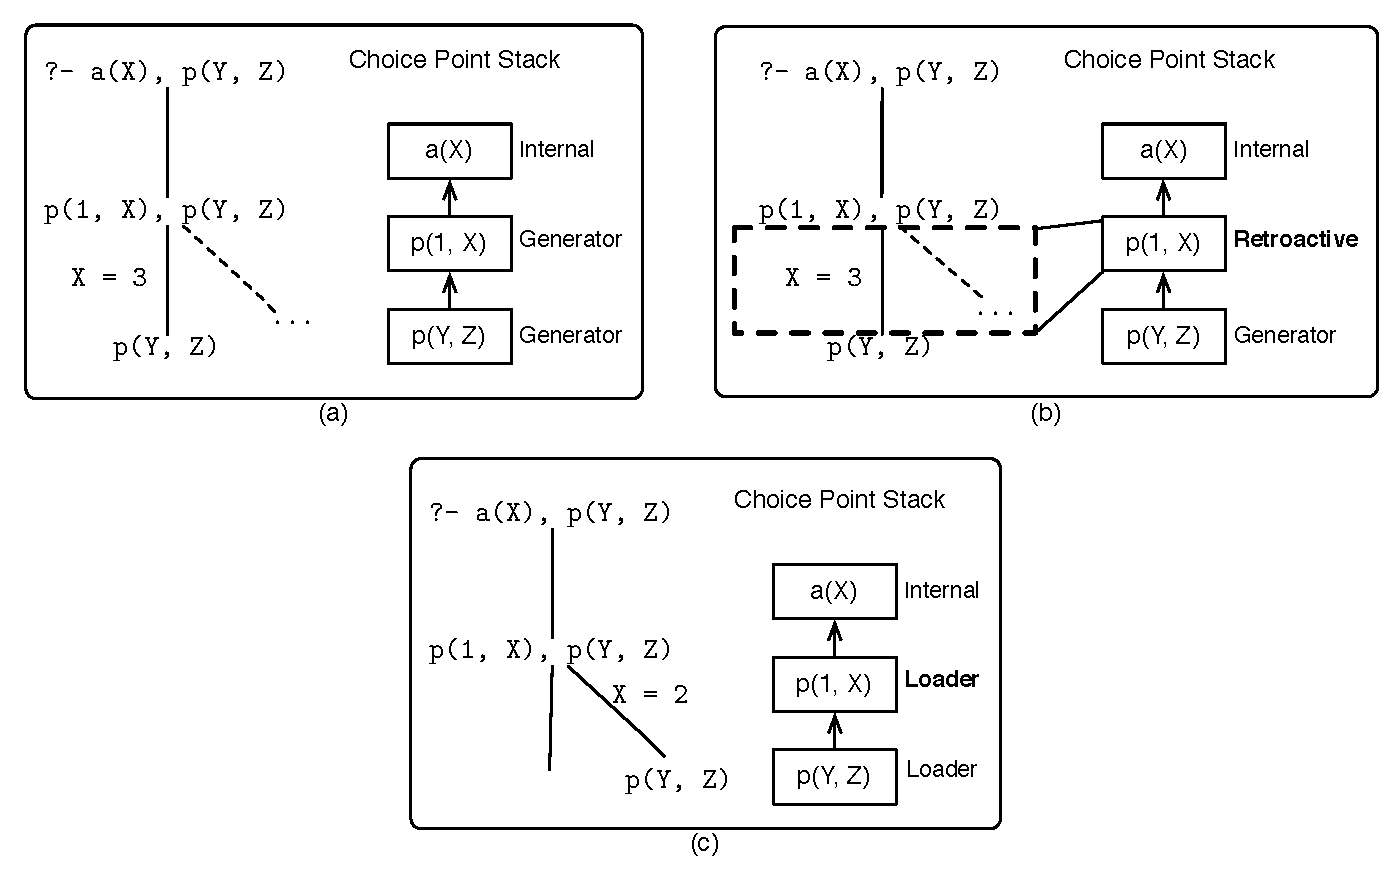
\includegraphics[scale=0.6]{pruning_example1.pdf}
  \caption{Evaluating `\texttt{a(X),~p(Y,Z)}' using retroactive tabling.}
  \label{fig:retro_eval1}
\end{figure}

The previous example has illustrated one special type of pruning called \textit{external pruning}.
External pruning occurs when the subsuming subgoal $G'$ is an \textit{external subgoal} to the evaluation
of the subsumed subgoal $G$. Another type of pruning is called \textit{internal pruning} and happens
when $G'$ is an \textit{internal subgoal} to the evaluation of $G$, that is, $G'$ is called
during the resolution of $G$. Although these two basic types of pruning can derive any other
situation, they both generate the same issues related to evaluation pruning. These issues will be explored
in detail in the next section.

\section{Pruning: Rules and Issues}

When pruning parts of the computation, we must know the areas of the local stack
that contain the choice points to prune. Given the nature of the tabling evaluation, choice points not
directly related to the pruned subgoal can get mixed with other choice points. This happens when a branch
containing external choice points has been suspended, but after backtracking to internal choice points we
execute a subsuming subgoal. Therefore, we must have a mechanism that can tell us if a certain choice
point is internal to a subgoal, from a range of choice points that can potentially contain choice points from
the pruned subgoal.

For this, we construct a dependency tree of subgoals and dependency frames by storing in a field
called \texttt{top\_gen} a pointer to the top tabled subgoal. Thus, by traversing this field we know
what subgoals the target subgoal or consumer is internal to.

When pruning execution branches, issues arise mostly when the computation of the subsumed subgoal involves
consumer and/or generators nodes. The next example programs will illustrate these issues.

Consider the program in Figure~\ref{fig:retro_program2} that mixes tabled predicates using retroactive
call subsumption and tabled predicates with variant checks.
For this program, we will use the query goal `\texttt{a(X,Y),~p(Z,W)}'.

\begin{figure}[ht]
\begin{Verbatim}
:- use_variant_tabling [a/2, b/1].
:- use_retroactive_tabling p/2.

a(X, Y) :- p(1, X), b(Y).
a(3, 4).

b(1).
b(2).

p(1, X) :- a(_, X).
p(1, X) :- b(X).
\end{Verbatim}
\caption{Example program using retroactive tabling with variant tabling.}
\label{fig:retro_program2}
\end{figure}

Initially, evaluation calls \texttt{a(X,Y)} and a new generator node is stored. Next, the retroactive subgoal
\texttt{p(1,X)} is called and creates a new generator node, because no subsuming subgoal is found.
The first clause of \texttt{p/2} executes \texttt{a(\_,X)}, which is a consumer of \texttt{a(X,Y)}, but, as
no answers are available to consume, execution suspends this node and backtracks to try to second clause
of \texttt{p/2}. Here, \texttt{b(X)} is called for the first time, creating a new generator choice point.
An answer for \texttt{b(X)} is generated, \texttt{\{X~=~1\}}, and by forward execution it is also an answer
for \texttt{p(1,X)}. Next, \texttt{b(Y)} is called, creating a new consumer node that consumes the answer
\texttt{\{X~=~1\}} and by forward execution, the first answer for \texttt{a(X,Y)}, \texttt{\{X~=~1,~Y~=~1\}},
is generated.

\begin{figure}[ht]
  \centering
    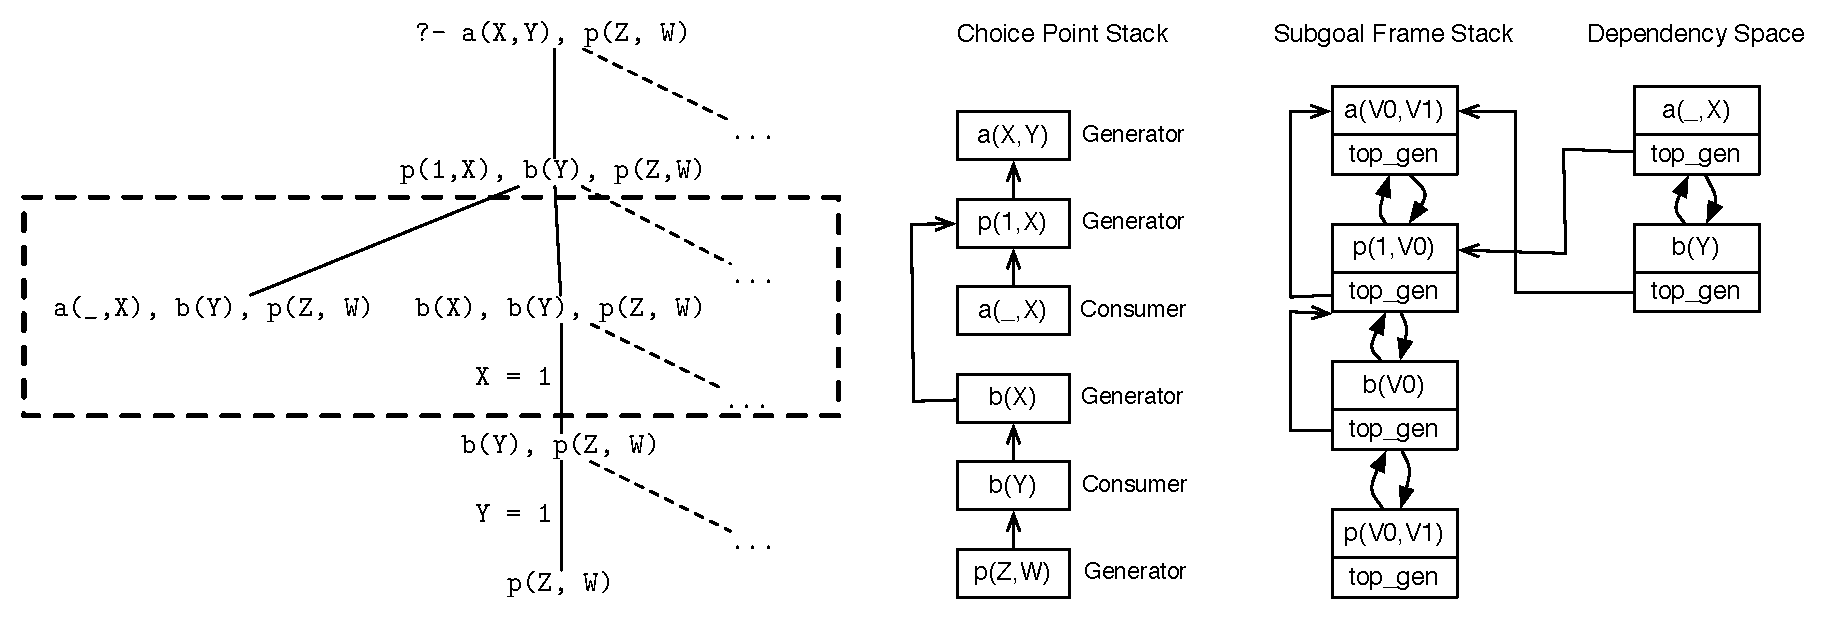
\includegraphics[scale=0.5]{retro_example2.pdf}
  \caption{Evaluating `\texttt{a(X,Y),~p(Z,W)}' using retroactive tabling.}
  \label{fig:retro_eval2}
\end{figure}

Next, subgoal \texttt{p(Z,W)} is called, which subsumes \texttt{p(1,X)} and the evaluation of this subgoal
must be pruned. Now, the subgoal \texttt{p(1,X)} includes various choice points involved in its computation,
namely \texttt{a(\_,X)} and \texttt{b(X)}.

The consumer node associated with the subgoal \texttt{a(\_,X)} must leave the computation and no longer
participates in answer resolution, thus its dependency frame is removed from the dependency space.

Pruning the generator node associated with the subgoal \texttt{b(X)} is a more tricky case. Notice that
the consumer \texttt{b(Y)} depends on this subgoal to consume new answers, thus by removing the generator node
the consumer will become an \textit{orphaned consumer} and the computation will complete too early.
Therefore, we mark the subgoal \texttt{b(X)} as \textit{pruned} and turn the consumer node of \texttt{b(Y)}
into a retroactive node.

Next, the subgoal \texttt{p(Z,W)} starts to execute the first clause of \texttt{p/2} and creates
a new consumer for \texttt{a(\_,X)}, that will consume one answer. By forward execution, an answer
for \texttt{p(Z,W)}, \texttt{\{Z~=~1,~W~=~1\}}, is generated. By means of backtracking, the second
clause of \texttt{p/2} is executed and calls \texttt{b(Y)}; as \texttt{b(Y)} is a pruned subgoal,
we first load the answers already generated for this subgoal and then execute the clauses of \texttt{b/1}.
After \texttt{b(Y)} generates all the answers, it completes successfully and execution backtracks to
\texttt{p(Z,W)}, to attempt completion of this subgoal. As the leader node is currently \texttt{a(X,Y)},
completion fails.

We backtrack to the retroactive node \texttt{b(Y)} will order to do retroactive resolution. Evaluation
notices that the subgoal has already completed, thus the retroactive node is transformed into a loader node
to consume all answers that were not consumed. By forward execution, a new consumer for \texttt{p(Z,W)} is
created that will generate more answers for the query goal. Once \texttt{b(Y)} does not have more answers
to consume, execution backtracks to the retroactive node of \texttt{p(1,X)}. Here, we note that
the producer subgoal, \texttt{p(Z,W)} has still not completed and this retroactive node must be turned
into a consumer node, which amounts to create a new dependency frame that is added into the dependency space,
in order to participate in the resolution process.

After \texttt{p(1,X)} executes the answer resolution
operation, evaluation backtracks to \texttt{a(X,Y)} that will execute the second clause of \texttt{a/2}.
Once \texttt{a(X,Y)} executes the completion operation and each each consumer has consumed its answers,
the subgoal completes and evaluation is finished.

\subsection{Pruning Actions}

The previous example has illustrated the different actions that must be applied to each choice point that
makes part of the computation of the subsumed subgoal. This action is dependent on the choice point
type and is summarized in the next subsections.

\subsubsection{Interior Nodes}

Interior nodes are related to normal Prolog execution and can be easily pruned
by ignoring them altogether. This approach, while simple, suffers from the problem of \textit{trapped
choice points}. This problem also affects delaying based tabling engines like YapTab and SLG-WAM, where
choice points under consumers are frozen and remain until completion. The CHAT approach to tabling
solves this problem by removing trapped choice points \cite{Demoen-99b}. Another solution would involve
modifications to the WAM garbage collector to collect unused space on the choice point stack.


\subsubsection{Internal Consumers}   
   
Internal consumers must be explicitly pruned by removing the associated
dependency frame from the dependency space. Thus prevents the resolution process to reactivate pruned
branches. In the previous example, \texttt{a(\_,X)} was an internal consumer.

\begin{figure}[ht]
\begin{Verbatim}
abolish_dependency_frames(specific_sg, min, max) {
   top = dependency_frame_before(specific_sg, max)

   while (top != NULL and younger_than(depfr_cons_cp(top), min))
      depfr = top
      top = depfr_next(depfr)

      if (is_internal_depfr(specific_sg, depfr, min))
         remove_from_stack(depfr)
         free(dep_fr)
}
\end{Verbatim}
\caption{Pseudo-code for procedure \texttt{abolish\_dependency\_frames}.}
\label{fig:abolish_dependency_frames}
\end{figure}
   
Figure~\ref{fig:abolish_dependency_frames} shows the procedure that abolishes internal dependency frames.
The arguments are: \texttt{specific\_sg}, the subsumed subgoal to prune; \texttt{min}, the first choice point address from the range of choice points to selectively prune; and \texttt{max}, the last choice point from the pruned range. First, we compute the first dependency frame inside the choice point range by using the function \texttt{dependency\_frame\_before}. Next, we iterate the dependency frames inside the range and check if they are internal to the choice point; if they are, we remove them from the dependency space.

\subsubsection{Internal Generators}

For internal generators we must remove its corresponding subgoal frame
from the subgoal frames stack and alter its state to pruned. Generally, when pruning internal generators, we
have two situations: (1) the generator does not have consumers that are external to the computation of the
subsumed subgoal; or (2) the generator has external consumers. The former situation does not introduce any
problem, but the latter origins orphaned consumers. In our example, the consumer node for \texttt{b(Y)} is
an orphaned consumer.

Usually, a pruned generator is called again during the evaluation of the subsuming subgoal, and before
the computation reaches any of the orphaned consumers. Once reactivated, the subgoal frame for the pruned
generator is pushed again into the top of the subgoal frame stack and its state is altered to
\textit{evaluating}. Then, the new generator node starts by consuming the previously generated answers
and only then executes the program clauses.

\begin{figure}[ht]
\begin{Verbatim}
abolish_subgoal_frames(specific_sg, min, max) {
   top = subgoal_frame_before(specific_sg, max)

   while (top != NULL and younger_or_equal(generator_cp(top), min))
      sg_fr = top
      top = next(sg_fr)

      if (is_internal_subgoal_frame(specific_sg, sg_fr, min))
         sg_cp = generator_cp(sg_fr)
         
         remove_subgoal_from_stack(sg_fr)
         
         if (type(sg_fr) == VARIANT or type(sg_fr) == RETROACTIVE)
            if (has_external_consumers(sg_fr))
               update_external_consumers(specific_sg, sg_fr, sg_cp, max)
               state(sg_fr) = pruned
            else
               free(sg_fr)
         else if (type(sg_fr) == SUBSUMPTIVE)
            if (has_proper_consumers(sg_fr))
               transform_external_subsumed_consumers(specific_sg, sg_fr, sg_cp, max)
            
            if (has_variant_consumers(sg_fr))
               update_external_consumers(specific_sg, sg_fr, sg_cp, max)
               
            if (has_no_consumers(sg_fr))
               free(sg_fr)
}
\end{Verbatim}
\caption{Pseudo-code for procedure \texttt{abolish\_subgoal\_frames}.}
\label{fig:abolish_subgoal_frames}
\end{figure}


\subsection{Orphaned Consumers}

\subsection{Lost Consumers}

\subsection{Frontier Choice Point}

\subsection{Leader Re-Computation}

\section{Internal Pruning}

\section{Mixing External and Internal Pruning}

\section{Table Space}

\section{Searching Subsumed Subgoals}

\section{Implementation Details}

\subsection{Retroactive Resolution}

\subsection{Subgoal Frames}

\subsection{External or Internal}

\subsection{Transforming Consumers Into Generators}

\subsection{Subgoal Dependency Tree}

\subsection{Reference Counting}

\chapter{Experimental Results}
This chapter presents a detailed performance analysis of our two subsumption-based tabling engines
that we have developed. We divided this chapter into four sections. The first section describes the
set of tabled benchmark programs used. The second
section evaluates the engine supporting traditional call subsumption that was implemented by integrating the
Time-Stamped Tries algorithms and data structures from XSB into Yap. This includes analyzing the memory gains
of call subsumption by measuring the size of the answer tries and comparing it to variant-based tabling.
In the third section, we evaluate the retroactive-based tabling engine for programs that do not benefit
from the new mechanisms and for programs that can take advantage of this new evaluation method. Finally,
in the fourth section we evaluate the STST table space overhead in a potentially not so good scenario,
where the operations of loading and storing answers are more expensive than usual.

\section{Benchmark Programs}

In order to assess the performance of our tabling engines we used various programs and data sets.
We next briefly describe the programs used (see Appendix~\ref{app:code} for more details).

\begin{description}
   
   \item[path:] This program computes the reachability between two nodes in a graph.
   Connections between two nodes are represented by \texttt{edge/2} facts.
   We used the following graph configurations in our tests: \textbf{tree}, a
   binary tree; \textbf{chain}, a chain of nodes; \textbf{cycle}, a chain of nodes, where the
   last node connects with the first one; \textbf{pyramid}, a pyramid like configuration;
   and \textbf{grid}, where nodes are connected in a grid-like fashion.
   For the \texttt{path/2} predicate itself, we used 6 different versions: \texttt{left\_first},
   \texttt{left\_last}, \texttt{right\_first}, \texttt{right\_last},
   \texttt{double\_first}, and \texttt{double\_last}.
    
   \item[samegen:] The \texttt{samegen/2} predicate solves the same generation problem.
   For this program, we used the configurations described above for \texttt{path}.
   
   \item[genome:] This program computes the set of nodes that are reachable by nodes 1 and 2 in a graph.
   This is an interesting problem, since it creates lots of subsumed consumers when using
   call subsumption. We also used the same configurations described above for \texttt{path}.
   To compute reachability this program uses a \texttt{left\_last} version.
   
   \item[reach:] The \texttt{reach/2} predicate computes the reachability in a relation graph for a set of
   model specifications. The benchmark is actually a set of programs originally taken from the
   XMC project~\cite{RamakrishnanCR-00}, which is a model checker implemented
   atop the XSB system. We used two variants of the \texttt{reach/2} predicate,
   \texttt{reach\_first} and \texttt{reach\_last}.
   The following relation graphs where used:
   
      \begin{description}
         
         \item[sieve:] \emph{sieve} specification defined for 5 processes and 4 overflow prime numbers.
         
         \item[leader:] \emph{leader election} specification defined for 5 processes.
         
         \item[iproto:] \emph{i-protocol} specification defined for a correct version with a huge window size.

      \end{description}
      
   \item[flora:] This program was generated by an object-oriented knowledge base language and application 
               development environment known as FLORA-2 \cite{Yang-00} \footnote{http://flora.sourceforge.net}.
               
   \item[fib:] This program uses a \texttt{fib/2} predicate to compute the Fibonacci number of a given
   parameter which allows to benchmark the pruning of one subsumed subgoal.
   
   \item[big:] This program also uses the \texttt{fib/2} predicate, but instead of one, multiple subsumed subgoals
   are called and pruned. As a parameter, we can input the number of subsumed subgoals to call and prune.
   
\end{description}

Again, Note that the relevant parts of the code for these programs are presented in Appendix~\ref{app:code}.

The environment for our experiments was an Intel Core(TM) 2 Quad 2.66 GHz with 4 GBytes of
memory and running the Linux kernel 2.6.31 with YapTab 6.0.3 and XSB Prolog 3.2.
The scheduling strategy used by default was batched scheduling.

\section{Traditional Call Subsumption with TST}

In this section, we first evaluate the performance of YapTab against the SLG-WAM,
by comparing the gains obtained by using call subsumption instead of variant checks.
In the second part of this section, we measure the impact in terms of space of using call subsumption.
For this, we compared the number of answer trie nodes created by using variant checks and by using subsumptive
checks.

\subsection{Performance Evaluation}

In order to compare the YapTab tabling engine with the SLG-WAM we used the following programs:

\begin{itemize}
   \item The \texttt{path/2} program with all the combinations of
   versions and data sets and the query goal `\texttt{?-~path(X,Y).}'.
   
   \item The \texttt{samegen/2} program with all data sets and the query goal `\texttt{?-~samegen(X,Y).}'.
   
   \item The \texttt{genome/1} program with all the data sets and the query goal `\texttt{?-~genome(X).}'.
   
   \item The two versions of the \texttt{reach/2} program with the following queries for each relation graphs:

   \begin{itemize}
      \item sieve: `\texttt{?-~reach(sieve\_0(5,4,27,end),Y).}'.
      \item leader: `\texttt{?-~reach(systemLeader\_0(5,end),Y).}'.
      \item iproto: `\texttt{?-~reach(iproto\_0(\_,\_,end),Y).}'.
   \end{itemize}

\end{itemize}

For each benchmark, we used variant-based tabling and then subsumption-based tabling.
Next, we computed the execution time and compared the speedups obtained ($T_{variant} / T_{subsumptive}$) for
each engine. The times presented next are the average of 3 runs. Given that YapTab's implementation
is largely based on XSB's code to implement the subsumption mechanisms,
we expect the speedups to be very similar. Some potential differences between them will arise because
of certain characteristics, namely: the way they implement the tabling algorithms, the WAM engine itself,
the compiled trie code, and the handling of answer templates.

Table~\ref{tbl:results_overview} summarizes the average speedups obtained for each program,
while Tables~\ref{tbl:result_detail_path} and \ref{tbl:result_detail_others}
show the full details, with times and speedups for YapTab and SLG-WAM.

\begin{table}[ht]
\centering
  \begin{tabular}{ccc}
   \hline
    \hline
    \multirow{2}{*}{\textbf{Program}} & \textbf{SLG-WAM} & \textbf{YapTab} \\
    & \textbf{\textit{\small{Average Speedup}}} & \textbf{\textit{\small{Average Speedup}}} \\
   \hline
   \hline
left\_first & 0.78 & \textbf{1.02} \\
left\_last & 0.77  & \textbf{0.96} \\
right\_first & \textbf{1.01} & \textbf{1.01} \\
right\_last & 0.94 & \textbf{1.07} \\
double\_first & 1.37 & \textbf{1.48} \\
double\_last & 1.31 & \textbf{1.40} \\
samegen & \textbf{339.76} & 1.03 \\
genome & 559.54 & \textbf{648.51} \\
reach\_first  & \textbf{0.96} & 0.94 \\
reach\_last  & \textbf{0.97} & 0.90 \\
\hline
\hline
\end{tabular}
\caption{Average speedups for call subsumption in SLG-WAM and YapTab.}
\label{tbl:results_overview}
\end{table}

The first thing we note is that,  YapTab has a better speedup than SLG-WAM in 6 benchmarks, while in 3 of
them SLG-WAM wins. In most of the benchmarks, the speedups for the two engines are very similar, which proves
that our integration efforts were  largely successful. However, for the \texttt{samegen} benchmark the
speedups are not very similar at all, the SLG-WAM engine has an average speedup of 339.76
and YapTab only 1.03. This happens because the performance of the variant-based version of SLG-WAM
performs very poorly against YapTab, which explains such big differences (see Table~\ref{tbl:result_detail_others}
for details).

The programs \texttt{left\_first} and \texttt{left\_last} do not generate any subsumed consumer,
therefore they are good benchmarks to assess the overhead of using the subsumption mechanisms. For YapTab,
the overhead is minimal with an average speedup of 0.96 for the \texttt{left\_last} program. Surprisingly, for the
\texttt{left\_first} program the speedup is 1.02, that is, the subsumptive-based engine performed better
than the variant-based engine. The SLG-WAM behavior for these two programs is clearly worst, with an average
speedup of 0.78 and 0.77 for \texttt{left\_first} and \texttt{left\_last}, respectively.

The programs \texttt{right\_first} and \texttt{right\_last} do generate subsumed consumers,
as many as the number of \texttt{edge/2} facts. Notably, only YapTab
achieves an average speedup bigger than 1 for both programs. These programs show poor speedups because simple facts
are faster to evaluate than to use the time stamped trie to collect relevant answers.
In particular, the binary tree graph configuration with the \texttt{right\_first} and \texttt{right\_last} programs
in YapTab has a very poor speedup of 0.93 and 0.33, respectively, which is clearly influencing the average speedups.
(see Table~\ref{tbl:result_detail_path}).
In the \texttt{right\_first} benchmark, the time stamped index is created right at
the beginning of the program, when the time stamped trie is still empty, and maintained thereafter, but,
in the case of the \texttt{right\_last} program, the indices are only created when the recursive
clause is executed, and at that time the trie already contains a considerable amount of answers.
We thus modified the subsumptive
engine to create the time stamp index from the beginning, and the \texttt{right\_last} program had considerable
better results. Therefore, we argue that the lazy creation of the time stamped index can affect considerably the
execution time, for programs where consumers appear when the answer trie already contains lots of answers.
The operation of creating the time stamped index
and sorting each trie node at each trie level can be very costly when a large number of nodes exist.
By experimentation we found that it seems more efficient to maintain the index as the answer trie is being expanded.

For the \texttt{double\_first} and \texttt{double\_last} we have attained speedups between 1.31 and 1.48
for both YapTab and SLG-WAM. These benchmarks are more computationally expensive given that they create more
dependencies. However, in subsumption-based tabling, the number of dependencies is reduced 
and thus no code is executed.

The \texttt{genome} program shows the best speedup results, with an impressive average speedup of 
648.51 for YapTab. In this program, the subgoal \texttt{path(2,X)} and \texttt{path(1,X)} are called
very early in the evaluation which makes all further subgoals calls to \texttt{path/2} that are subsumed by these
goals as consumers.

For the model checking programs, the results were not so good with close speedups for YapTab and SLG-WAM.

\begin{table}[ht]
\centering
\footnotesize{
  \begin{tabular}{cc|ccc|ccc}
   \hline
    \hline
    \multicolumn{2}{c|}{\multirow{2}{*}{\small{\textbf{Data}}}} & \multicolumn{3}{c|}{\small{\textbf{SLG-WAM}}} & \multicolumn{3}{c}{\small{\textbf{YapTab}}} \\
     \multicolumn{2}{c|}{} & \textbf{\textit{Var}} & \textbf{\textit{Sub}} & \textbf{\textit{Speedup}} & \textbf{\textit{Var}} & \textbf{\textit{Sub}} & \textbf{\textit{Speedup}} \\
   \hline
   \hline
   \multirow{5}{*}{\textbf{left\_first}} &  \scriptsize{chain  (4096) }  &  2793 & 3869 &  0.72  & 2688 & 2533 &  \textbf{1.06} \\
   &  \scriptsize{cycle  (4096) }  &  6201 & 9561 &  0.65  & 7260 & 6100 &  \textbf{1.19} \\
   &  \scriptsize{grid  (64) }  &  15416 & 16003 &  \textbf{0.96}  & 10702 & 11638 &  0.92 \\
   &  \scriptsize{pyramid  (4096) }  &  9565 & 13849 &  0.69  & 13550 & 13462 &  \textbf{1.01} \\
   &  \scriptsize{tree  (32768) }  &  140 & 161 &  0.87  & 129 & 142 &  \textbf{0.91} \\
   \hline
   \multirow{5}{*}{\textbf{left\_last}} &  \scriptsize{chain  (4096) }  &  2766 & 3900 &  0.71  & 2666 & 2505 &  \textbf{1.06} \\
   &  \scriptsize{cycle  (4096) }  &  5724 & 9273 &  0.62  & 7042 & 6394 &  \textbf{1.10} \\
   &  \scriptsize{grid  (64) }  &  13609 & 15670 &  \textbf{0.87}  & 10801 & 12396 &  \textbf{0.87} \\
   &  \scriptsize{pyramid  (2048) }  &  2385 & 2958 &  0.81  & 2904 & 3112 &  \textbf{0.93} \\
   &  \scriptsize{tree  (32768) }  &  133 & 156 &  \textbf{0.85}  & 122 & 145 &  0.84 \\
   \hline

   \multirow{5}{*}{\textbf{right\_first}} &  \scriptsize{chain  (4096) }  &  2830 & 3030 &  0.93  & 3253 & 3434 &  \textbf{0.95} \\
   &  \scriptsize{cycle  (4096) }  &  6313 & 7012 &  0.90  & 7090 & 6648 &  \textbf{1.07} \\
   &  \scriptsize{grid  (64) }  &  21318 & 15282 &  \textbf{1.39}  & 16659 & 16091 &  1.04 \\
   &  \scriptsize{pyramid  (4096) }  &  10348 & 10617 &  0.97  & 12781 & 11677 &  \textbf{1.09} \\
   &  \scriptsize{tree  (32768) }  &  157 & 180 &  0.87  & 217 & 237 &  \textbf{0.92} \\
   \hline
   \multirow{5}{*}{\textbf{right\_last}} &  \scriptsize{chain  (4096) }  &  2864 & 2970 &  0.96  & 4032 & 3672 &  \textbf{1.10} \\
   &  \scriptsize{cycle  (4096) }  &  6373 & 7036 &  0.91  & 8362 & 6654 &  \textbf{1.26} \\
   &  \scriptsize{grid  (64) }  &  18346 & 13374 &  1.37  & 19741 & 13286 &  \textbf{1.49} \\
   &  \scriptsize{pyramid  (4096) }  &  10548 & 10900 &  0.97  & 13496 & 11397 &  \textbf{1.18} \\
   &  \scriptsize{tree  (65536) }  &  \scriptsize{crashed} & \scriptsize{crashed} &  ---  & 478 & 1458 &  0.33 \\
   \hline
   
   \multirow{5}{*}{\textbf{double\_first}} &  \scriptsize{chain  (512) }  &  5070 & 3546 &  \textbf{1.43}  & 3626 & 2705 &  1.34 \\
   &  \scriptsize{cycle  (512) }  &  31053 & 20431 &  1.52  & 36334 & 15141 &  \textbf{2.40} \\
   &  \scriptsize{grid  (16) }  &  3906 & 2594 &  \textbf{1.51}  & 2762 & 1845 &  1.50 \\
   &  \scriptsize{pyramid  (512) }  &  22507 & 14176 &  1.59  & 19341 & 11589 &  \textbf{1.67} \\
   &  \scriptsize{tree  (32768) }  &  773 & 961 &  \textbf{0.80}  & 756 & 1602 &  0.47 \\
   \hline
   \multirow{5}{*}{\textbf{double\_last}} &  \scriptsize{chain  (512) }  &  5032 & 3553 &  \textbf{1.42}  & 3638 & 2578 &  1.41 \\
   &  \scriptsize{cycle  (512) }  &  30991 & 20881 &  1.48  & 31302 & 16918 &  \textbf{1.85} \\
   &  \scriptsize{grid  (16) }  &  4048 & 2697 &  \textbf{1.50}  & 2510 & 1882 &  1.33 \\
   &  \scriptsize{pyramid  (512) }  &  20518 & 15255 &  1.35  & 19969 & 10586 &  \textbf{1.89} \\
   &  \scriptsize{tree  (32768) }  &  766 & 972 &  \textbf{0.79}  & 730 & 1453 &  0.50 \\
   \hline


\hline
\end{tabular}
}
\caption{Times and speedups for call subsumption in SLG-WAM and YapTab: \texttt{path} programs.}
\label{tbl:result_detail_path}
\end{table}

\begin{table}[ht]
\centering
\footnotesize{
  \begin{tabular}{cc|ccc|ccc}
   \hline
    \hline
    \multicolumn{2}{c|}{\multirow{2}{*}{\small{\textbf{Data}}}} & \multicolumn{3}{c|}{\small{\textbf{SLG-WAM}}} & \multicolumn{3}{c}{\small{\textbf{YapTab}}} \\
     \multicolumn{2}{c|}{} & \textit{Var} & \textit{Sub} & \textit{Speedup} & \textit{Var} & \textit{Sub} & \textit{Speedup} \\
   \hline
   \hline
   
   \multirow{5}{*}{samegen} &  \scriptsize{chain  (32768) }  &  23439 & 22 &  \textbf{1065.41}  & 57 & 58 &  0.98 \\
   &  \scriptsize{cycle  (16384) }  &  6046 & 12 &  \textbf{503.83}  & 38 & 33 &  1.15 \\
   &  \scriptsize{grid  (32) }  &  2234 & 1362 &  \textbf{1.64}  & 1437 & 1205 &  1.19 \\
   &  \scriptsize{pyramid  (4096) }  &  2286 & 18 &  \textbf{127.00}  & 25 & 21 &  1.19 \\
   &  \scriptsize{tree  (8192) }  &  8037 & 8785 &  \textbf{0.91}  & 4856 & 7605 &  0.64 \\
   \hline
   
   \multirow{5}{*}{genome} &  \scriptsize{chain  (16384) }  &  9276 & 18 &  515.33  & 21133 & 16 &  \textbf{1320.81} \\
   &  \scriptsize{cycle  (8192) }  &  2356 & 8 &  294.50  & 4744 & 8 &  \textbf{593.00} \\
   &  \scriptsize{grid  (64) }  &  1098 & 8 &  137.25  & 1733 & 12 &  \textbf{144.42} \\
   &  \scriptsize{pyramid  (4096) }  &  1957 & 8 &  244.62  & 2229 & 8 &  \textbf{278.62} \\
   &  \scriptsize{tree  (32768) }  &  41756 & 26 &  \textbf{1606.00}  & 47097 & 52 &  905.71 \\
   \hline

   \multirow{3}{*}{reach\_first} &  \scriptsize{iproto }  &  2533 & 2582 &  \textbf{0.98}  & 1321 & 1433 &  0.92 \\
   &  \scriptsize{leader }  &  5797 & 6042 &  \textbf{0.96}  & 2304 & 2420 &  0.95 \\
   &  \scriptsize{sieve }  &  17822 & 19099 &  0.93  & 14130 & 14880 &  \textbf{0.95} \\
   \hline
   \multirow{3}{*}{reach\_last} &  \scriptsize{iproto }  &  2428 & 2558 &  \textbf{0.95}  & 1177 & 1426 &  0.83 \\
   &  \scriptsize{leader }  &  5786 & 6005 &  \textbf{0.96}  & 2170 & 2504 &  0.87 \\
   &  \scriptsize{sieve }  &  18027 & 17945 &  1.00  & 14888 & 14782 &  \textbf{1.01} \\
   \hline
\hline
\end{tabular}
}
\caption{Times, in milliseconds, and speedups for call subsumption in SLG-WAM and YapTab: \textbf{samegen}, \textbf{genome}, and model checking programs.}
\label{tbl:result_detail_others}
\end{table}

\subsection{Memory usage}

In this section we measure the size of the table space, for the variant and the subsumptive engine.
As a metric, we use the number of allocated answer trie nodes across all answer tries.
For this, we used the following benchmarks:

\begin{itemize}
   \item The programs \texttt{left\_first}, \texttt{right\_first} and \texttt{double\_first} with the query `\texttt{?-~path(X,Y).}'. Note that there is no need to use
   the \texttt{last} versions of these programs, because they will result in the same number of answer trie nodes.
   
   \item The \texttt{samegen/2} program.
   
   \item The \texttt{genome/1} program.
   
   \item The \texttt{flora} benchmark.
\end{itemize}

Table~\ref{tbl:results_detail_space_sub} presents the results we obtained. From the table, we see that,
for some programs where no subsumed subgoals are called, the number of answer trie nodes created is
exactly same when compared to variant-based tabling. For example, in the programs \texttt{genome/1} and
\texttt{left\_first} we can observe this behavior. Please notice that, while the number of trie nodes is
the same, the size of the nodes in subsumption-based tabling (they have a \textbf{timestamp} field) make
the time stamped answer trie more costly in terms of memory used.

In the programs \texttt{right\_first} and \texttt{double\_first}, the number of answer trie nodes
is reduced in half. Using variant-based tabling, these programs generate a large number of subgoals,
that in subsumption-based tabling are consumers of the first called subgoal, thus creating more
answer tries for each one of these subgoals, and thus more answer trie nodes. As one would expect,
using subsumption-based tabling can reduce substantially the table space.

The \texttt{samegen/2} program presents a curious behavior for the \texttt{cycle} and \texttt{chain}
data sets. In these cases, the program generates an answer that subsumes all the other answers and
every other subgoal call is subsumed by the top subgoal, resulting in only 3 answer trie nodes created,
the root node, and the two nodes for the two terms of the general solution. Compared to tabling with
variant checks, this result in very good space savings.
The \texttt{flora} benchmark also shows a reduced table space size, which shows that subsumption-based
tabling can be successfully applied to complex programs, resulting in a largely reduced
table space.

\begin{table}[ht]
\centering
\small{
  \begin{tabular}{cc|ccc}
   \hline
    \hline
    \multicolumn{2}{c|}{\multirow{2}{*}{\normalsize{\textbf{Data}}}} & \multicolumn{3}{c}{\normalsize{\textbf{YapTab}}} \\
     \multicolumn{2}{c|}{} & \textit{\small{Var}} & \textit{\small{Sub}} & \textit{\small{Sub / Var}} \\
   \hline
   \hline
   
   \multirow{5}{*}{left\_first} &  \footnotesize{chain (4096)} &  8390656 & 8390656 &  1.00000 \\
   &  \footnotesize{cycle (4096)} &  16781313 & 16781313 &  1.00000 \\
   &  \footnotesize{grid (64)} &  16781313 & 16781313 &  1.00000 \\
   &  \footnotesize{pyramid (4096)} &  25171968 & 25171968 &  1.00000 \\
   &  \footnotesize{tree (32768)} &  442370 & 442370 &  1.00000 \\
   \hline

   \multirow{5}{*}{right\_first} &  \footnotesize{chain (4096)} &  16777216 & 8390656 &  0.50012 \\
   &  \footnotesize{cycle (4096)} &  33562625 & 16781313 &  0.50000 \\
   &  \footnotesize{grid (64)} &  33562625 & 16781313 &  0.50000 \\
   &  \footnotesize{pyramid (4096)} &  50335744 & 25171968 &  0.50008 \\
   &  \footnotesize{tree (32768)} &  868356 & 442370 &  0.50943 \\
   \hline
   
   \multirow{5}{*}{double\_first} &  \footnotesize{chain (512)} &  262144 & 131328 &  0.50098 \\
   &  \footnotesize{cycle (512)} &  525313 & 262657 &  0.50000 \\
   &  \footnotesize{grid (16)} &  131585 & 65793 &  0.50000 \\
   &  \footnotesize{pyramid (512)} &  786944 & 393984 &  0.50065 \\
   &  \footnotesize{tree (32768)} &  868356 & 442370 &  0.50943 \\
   \hline
   
   \multirow{5}{*}{samegen} &  \footnotesize{chain (32768)} &  131071 & 3 &  0.00002 \\
   &  \footnotesize{cycle (16384)} &  65539 & 3 &  0.00005 \\
   &  \footnotesize{grid (32)} &  1050627 & 524291 &  0.49903 \\
   &  \footnotesize{pyramid (4096)} &  49147 & 16383 &  0.33335 \\
   &  \footnotesize{tree (8192)} &  27974313 & 22369623 &  0.79965 \\
   \hline
   
   \multirow{5}{*}{genome} &  \footnotesize{chain (16384)} &  65533 & 49151 &  0.75002 \\
   &  \footnotesize{cycle (8192)} &  32771 & 24580 &  0.75005 \\
   &  \footnotesize{grid (64)} &  16387 & 12292 &  0.75011 \\
   &  \footnotesize{pyramid (4096)} &  24575 & 16385 &  0.66673 \\
   &  \footnotesize{tree (32768)} &  98299 & 65534 &  0.66668 \\
   \hline
  
\multicolumn{2}{c|}{flora} & 83564 & 30228 & 0.36173 \\
\hline
\hline
\end{tabular}
}
\caption{Number of stored answer trie nodes for variant and subsumption-based tabling in YapTab.}
\label{tbl:results_detail_space_sub}
\end{table}


\section{Performance Evaluation for RCS}

In this section we evaluate our retroactive-based tabling engine that we implemented on
top of YapTab. First, we start by assessing the overhead of using the new mechanisms that
support the RCS engine, namely: building the subgoal dependency tree, the STST table space,
and searching for running subsumed subgoals. In the second part of this section, we evaluate
the RCS engine with programs where specific subgoals are called before general subgoals, in
order to assess the advantages of the new mechanism.

\subsection{RCS Overhead}

To measure the overhead, we executed programs where general subgoals are always called before
subsumed subgoals (or not at all), therefore we can estimate the impact in the execution time
because the pruning techniques of RCS are not employed.
We used the following benchmarks:

\begin{itemize}
   \item Every combination of versions and data sets for the \texttt{path/2} program with the query `\texttt{?-~path(X,Y).}'.
   
   \item The query `\texttt{?-~samegen(X,Y).}' in the \texttt{samegen/2} program. All \texttt{path/2} data
   sets were used.
   
   \item The two versions of the \texttt{reach/2} program with the following queries for the relation graphs:

   \begin{itemize}
      \item sieve: `\texttt{?-~reach(sieve\_0(5,4,27,end),Y).}'.
      \item leader: `\texttt{?-~reach(systemLeader\_0(5,end),Y).}'.
      \item iproto: `\texttt{?-~reach(iproto\_0(\_,\_,end),Y).}'.
   \end{itemize}
\end{itemize}

We timed the execution of the benchmarks for the RCS engine and then the execution time
for the subsumptive and variant-based engines of both YapTab and SLG-WAM. All execution times are
the average of 3 runs. For each table,
we present the execution time of the RCS engine in milliseconds and the relative time
of the other engines by computing the value $T_{engine} / T_{RCS}$.
If the value is lesser than 1.0 then RCS performs worse, otherwise if the value is greater than
1.0 then RCS performs better. At the end of each table, we present the average values for
each engine.

Table~\ref{tbl:overhead_overview} shows the average overhead values computed for each benchmark program
for call subsumption in the SLG-WAM and in the YapTab engine. The detailed results are presented
in Tables~\ref{tbl:overhead_detail_tst} and \ref{tbl:overhead_detail_model}.
By analyzing the results we can see that YapTab with RCS performs worse
than YapTab with subsumptive-based tabling in most cases, and only the
programs \texttt{right\_first} and the \texttt{right\_last} program show better results,
while the \texttt{left\_first} and \texttt{left\_last} programs have very comparable execution times.
In theory, these benchmarks should not run faster, but cache effects and other
conditions could affect positively the execution time of these programs.

The average values presented in Table~\ref{tbl:overhead_overview} show that
RCS is very competitive against SLG-WAM, because SLG-WAM is in average 21\% slower than RCS. More
importantly, when comparing RCS to YapTab with traditional call subsumption, RCS performs 4\% slower,
which shows that RCS adds a very small overhead when executing programs that do not benefit from the
new evaluation model.

\begin{table}[ht]
\centering
  \begin{tabular}{ccc}
   \hline
    \hline
    \multirow{2}{*}{\textbf{Program}} & \textbf{SLG-WAM} & \textbf{YapTab} \\
    & \textbf{\textit{\small{Sub / Retro}}} & \textbf{\textit{\small{Sub / Retro}}} \\
   \hline
   \hline
   left\_first & 1.29 & 0.99 \\
   left\_last &  1.26  & 0.98 \\
   right\_first & 0.95 & \textbf{1.05} \\
   right\_last & 1.03 & \textbf{1.08} \\
   double\_first & 1.05 & 0.87 \\
   double\_last & 1.06 & 0.87 \\
   samegen & 0.75 & 0.90 \\
   reach\_first  &  1.78  & 0.96 \\
   reach\_last  &  1.73  & 0.96 \\
\hline
\hline
\textit{Average} &  1.21 &  0.96 \\
\hline
\hline
\end{tabular}
\caption{Average overhead values for programs do not take advantage of RCS.}
\label{tbl:overhead_overview}
\end{table}

\begin{table}[ht]
\centering
\small{
  \begin{tabular}{cc|ccc}
   \hline
    \hline
    \multicolumn{2}{c|}{\multirow{2}{*}{\normalsize{\textbf{Data}}}} & \multicolumn{3}{c}{\normalsize{\textbf{YapTab}}} \\
     \multicolumn{2}{c|}{} & \small{\textit{Retro}} & \textit{\small{Retro / Var}} & \textit{\small{Retro / Sub}} \\
   \hline
   \hline
   
   \multirow{5}{*}{left\_first} &  \footnotesize{chain  (4096) } &  2560 &  \textbf{0.96}  &  1.02 \\
   &  \footnotesize{cycle  (4096) } &  6357 &  \textbf{0.93}  &  1.05 \\
   &  \footnotesize{grid  (64) } &  12074 &  1.13  &  1.04 \\
   &  \footnotesize{pyramid  (4096) } &  13037 &  1.02  &  \textbf{0.92} \\
   &  \footnotesize{tree  (32768) } &  149 &  1.26  &  1.02 \\
   \hline
   \multirow{5}{*}{left\_last} &  \footnotesize{chain  (4096) } &  2577 &  \textbf{0.97}  &  1.05 \\
   &  \footnotesize{cycle  (4096) } &  6696 &  \textbf{0.98}  &  1.07 \\
   &  \footnotesize{grid  (64) } &  12072 &  1.12  &  \textbf{0.98} \\
   &  \footnotesize{pyramid  (2048) } &  2792 &  \textbf{0.97}  &  \textbf{0.96} \\
   &  \footnotesize{tree  (32768) } &  153 &  1.30  &  1.09 \\
   \hline

   \multirow{5}{*}{right\_first} &  \footnotesize{chain  (4096) } &  3109 &  \textbf{0.95}  &  \textbf{0.92} \\
   &  \footnotesize{cycle  (4096) } &  6894 &  \textbf{0.97}  &  1.03 \\
   &  \footnotesize{grid  (64) } &  14720 &  \textbf{0.89}  &  \textbf{0.88} \\
   &  \footnotesize{pyramid  (4096) } &  11578 &  \textbf{0.96}  &  \textbf{1.00} \\
   &  \footnotesize{tree  (32768) } &  212 &  1.07  &  \textbf{0.92} \\
   \hline
   \multirow{5}{*}{right\_last} &  \footnotesize{chain  (4096) } &  3144 &  \textbf{0.80}  &  \textbf{0.84} \\
   &  \footnotesize{cycle  (4096) } &  6225 &  \textbf{0.79}  &  \textbf{0.95} \\
   &  \footnotesize{grid  (64) } &  12265 &  \textbf{0.63}  &  \textbf{0.88} \\
   &  \footnotesize{pyramid  (4096) } &  11085 &  \textbf{0.83}  &  \textbf{0.97} \\
   &  \footnotesize{tree  (65536) } &  1376 &  3.19  &  1.04 \\
   \hline

   \multirow{5}{*}{double\_first} &  \footnotesize{chain  (512) } &  2925 &  \textbf{0.81}  &  1.08 \\
   &  \footnotesize{cycle  (512) } &  20513 &  \textbf{0.57}  &  1.36 \\
   &  \footnotesize{grid  (16) } &  2112 &  \textbf{0.76}  &  1.15 \\
   &  \footnotesize{pyramid  (512) } &  12990 &  \textbf{0.69}  &  1.13 \\
   &  \footnotesize{tree  (32768) } &  1606 &  2.24  &  1.07 \\
   \hline
   \multirow{5}{*}{double\_last} &  \footnotesize{chain  (512) } &  2976 &  \textbf{0.81}  &  1.09 \\
   &  \footnotesize{cycle  (512) } &  20963 &  \textbf{0.67}  &  1.29 \\
   &  \footnotesize{grid  (16) } &  2116 &  \textbf{0.84}  &  1.13 \\
   &  \footnotesize{pyramid  (512) } &  12062 &  \textbf{0.66}  &  1.14 \\
   &  \footnotesize{tree  (32768) } &  1564 &  2.22  &  1.13 \\
   \hline
\hline
\end{tabular}
}
\caption{Times, in milliseconds, and overheads for RCS in YapTab: \textbf{path} programs.}
\label{tbl:overhead_detail_tst}
\end{table}
\begin{table}[ht]
\centering
\footnotesize{
  \begin{tabular}{cc|c|cc|cc}
   \hline
    \hline
    \multicolumn{2}{c|}{\multirow{2}{*}{\small{\textbf{Data}}}} & \textbf{\small{Retro}} & \multicolumn{2}{c|}{\small{\textbf{SLG-WAM}}} & \multicolumn{2}{c}{\small{\textbf{YapTab}}} \\
     \multicolumn{2}{c|}{} & \scriptsize{\textit{milliseconds}} & \textbf{\textit{\scriptsize{Var / Retro}}} & \textbf{\textit{\scriptsize{Sub / Retro}}} & \textbf{\textit{\scriptsize{Var / Retro}}} & \textbf{\textit{\scriptsize{Sub / Retro}}} \\
   \hline
   \hline

   \multirow{5}{*}{\textbf{samegen}} &  chain  (32768)  &  65 &  360.46  &  0.38  &  0.75 &  0.89 \\
   &  cycle  (16384)  &  36 &  169.22  &  0.33  &  1.03 &  0.81 \\
   &  grid  (32)  &  1162 &  1.93  &  1.17  &  1.24 &  \textbf{1.03} \\
   &  pyramid  (4096)  &  30 &  76.17  &  0.60  &  0.70 &  0.70 \\
   &  tree  (8192)  &  6970 &  1.14  &  1.26  &  0.70 &  \textbf{1.09} \\
   \hline
   
   \multirow{3}{*}{\textbf{reach\_first}} &  iproto  &  1570 &  1.61  &  1.64  &  0.84 &  0.91 \\
   &  leader  &  2514 &  2.31  &  2.40  &  0.92 &  0.96 \\
   &  sieve  &  14644 &  1.22  &  1.30  &  0.96 &  \textbf{1.02} \\
   \hline
   \multirow{3}{*}{\textbf{reach\_last}} &  iproto  &  1585 &  1.53  &  1.61  &  0.74 &  0.90 \\
   &  leader  &  2560 &  2.26  &  2.35  &  0.85 &  0.98 \\
   &  sieve  &  14648 &  1.23  &  1.23  &  1.02 &  \textbf{1.01} \\

\hline
\end{tabular}
}
\caption{Detailed overhead results: \texttt{samegen} and model checking programs.}
\label{tbl:overhead_detail_model}
\end{table}

\subsection{RCS Gains}

In this section, we present experimental results using retroactive-based tabling on programs that
can benefit from it, i.e., programs where some general subgoal is called after a more specific subgoal.
The programs we used for these experiments are the following:

\begin{itemize}
   \item The programs \texttt{left\_first}, \texttt{left\_last},
   \texttt{double\_first} and \texttt{double\_last} with the query goal `\texttt{?-~path(X,1).}'.
   When calling the subgoal \texttt{path(X,1)}, the subgoal
   \texttt{path(X,Y)} is called, which prunes the first subgoal.
   
   \item The \texttt{genome/1} program with the query goal `\texttt{?-~genome(X).}'.
   
   \item The two versions of the \texttt{reach/2} program with the following pair of queries/relation graphs:

   \begin{itemize}
      \item sieve: `\texttt{?-~reach(sieve\_0(5,4,27,end),~par(A,~B,~C,~D)).}'.
      \item leader: `\texttt{?-~reach(systemLeader\_0(5,end),~par(D,~E,~A,~B)).}'.
      \item iproto: `\texttt{?-~reach(iproto\_0(\_,\_,end),imain\_7\_0(A,~B,~C,~D,~E)).}'.
   \end{itemize}
   
   \item The \textbf{flora} program with the query goal `\texttt{?-~\'\_\$\_\$\_flora\_isa\_rhs\'(\_,direct).}'.
   
   \item The \textbf{fib} program with the following parameters: 30, 32, 35, and 36. We use the following
   query goal: `\texttt{?-~a(X),~p(Y,~Z).}'.
   
   \item The \textbf{big} program with the following parameters (number of subgoals to prune): 5, 10, and 20.
   We use the query goal `\texttt{?-~a(X).}'
\end{itemize}

As the tables of the previous section, we present the results with the execution time of the retroactive-based
engine, along with the relative results for the SLG-WAM and YapTab engines, with both variant and subsumptive checks.
Execution times are an average of 3 runs.
In tables~\ref{tbl:results_detail_gain_tst}, \ref{tbl:results_detail_gain_model} and \ref{tbl:results_detail_gain_fib}
we show the detailed results of the experiments. Table~\ref{tbl:results_gain_overview} presents the average values of
each program.

\begin{table}[ht]
\centering
  \begin{tabular}{ccc}
   \hline
    \hline
    \multirow{2}{*}{\textbf{Program}} & \textbf{SLG-WAM} & \textbf{YapTab} \\
    & \textbf{\textit{\small{Sub / Retro}}} & \textbf{\textit{\small{Sub / Retro}}} \\
   \hline
   \hline
   
left\_first & 1.19 & 0.95 \\
left\_last & 1.23  & 0.90 \\
double\_first & 1.17 & \textbf{1.09} \\
double\_last & 1.14 & \textbf{1.10} \\
genome & 0.62 & 0.74 \\
reach\_first  & 3.52 & \textbf{1.76} \\
reach\_last  & 3.34 & \textbf{1.87} \\
flora & 0.29 & \textbf{1.17} \\
fib & 1.64 & \textbf{2.02} \\
big & 17.72 & \textbf{13.66} \\
\hline
\hline
\end{tabular}
\caption{Average benchmarks results for programs that take advantage of RCS.}
\label{tbl:results_gain_overview}
\end{table}

For the \texttt{path/2} we should make two distinctions. The versions where the recursive clause is the first
clause (\texttt{left\_first} and \texttt{double\_first}) and the versions with the recursive last as the second
clause (\texttt{left\_last} and \texttt{double\_last}). In the \texttt{first} versions, the specific subgoal
generates answers before reaching the general subgoal, while in the \texttt{last} versions, the general subgoal
is found right at the beginning. Therefore, the \texttt{first} versions should, in principle, attain more performance,
because they waste less time executing the subsumed subgoal. The results for the \texttt{left} versions of the
\texttt{path/2} program attest this, with speedups of 0.95 and 0.90 for the \texttt{left\_first} and
\texttt{left\_last} versions, respectively. Surprisingly, the \texttt{double} version has the opposite behavior.

Another important conclusion we can make from the results is that RCS may not show performance gains, even if the
programs can, in theory, take advantage of it. In our experiments, only the programs \texttt{left\_first},
\texttt{left\_last} and \texttt{genome} show, in average, worse performance.

We argue that the speedup of using RCS is highly dependent on the nature of the program.
The \texttt{left} version
of the \texttt{path/2} program, for example, does not show improvements because what we gain from pruning the
execution of simple \texttt{edge/2} facts does not offset the cost of using the STST to retrieve relevant answers
for the subsumed subgoal and
the cost of pruning the computation itself. In other words, using subsumptive-based tabling for this program is
advantageous because the cost of executing predicate clauses is less than maintaining the time stamped index.
Hence, for RCS to show improvements, the time that is wasted by executing pruned code should be greater than the
time spent manipulating the STST.

The model checking programs, \texttt{reach\_left} and \texttt{reach\_last}, are much more complex than the \texttt{path/2}
programs, and thus show much larger improvements. For the \texttt{reach\_last} program with the \texttt{leader} model,
we obtain a good speedup of 2.16. Also, the \texttt{flora} program also shows improvements with a speedup of 1.17 over
traditional call subsumption in YapTab. These complex benchmarks show that RCS has the potential to speedup the
execution on this type of programs.

The \textbf{fib} program shows a considerable average speedup of 2.19 for YapTab with call subsumption.
We can see that, for different parameters, the speedup is identical because the execution time of the pruned subsumed
subgoal is more or less equal to that of the subsuming subgoal. For the \textbf{big} program, where multiple
subsumed subgoals are pruned, we can see that as the number of pruned subsumed subgoals increases, the speedup
also increases, reaching a maximum of 21.24 for YapTab. An interesting observation for the \textbf{big} program is
that the execution time for retroactive-tabling stays the same, even if the number of subsumed subgoals to prune
increase.

Even if the \texttt{path/2} programs, in average, do not show considerable improvements, for some data sets
these programs can obtain good speedups, for example, the binary tree configuration can reach a speedup of 1.61.

\begin{table}[ht]
\centering
\small{
  \begin{tabular}{cc|ccc}
   \hline
    \hline
    \multicolumn{2}{c|}{\multirow{2}{*}{\normalsize{\textbf{Data}}}} & \multicolumn{3}{c}{\normalsize{\textbf{YapTab}}} \\
     \multicolumn{2}{c|}{} & \small{\textit{Retro}} & \textit{\small{Var / Retro}} & \textit{\small{Sub / Retro}} \\
   \hline
   \hline

   \multirow{5}{*}{left\_first} &  \footnotesize{chain  (4096) } &  2976 &  0.95  &  0.91 \\
   &  \footnotesize{cycle  (4096) } &  7020 &  0.77  &  0.75 \\
   &  \footnotesize{grid  (64) } &  13444 &  0.94  &  \textbf{1.00} \\
   &  \footnotesize{pyramid  (4096) } &  16562 &  0.87  &  0.93 \\
   &  \footnotesize{tree  (32768) } &  174 &  0.93  &  \textbf{1.16} \\
   \hline
   \multirow{5}{*}{left\_last} &  \footnotesize{chain  (4096) } &  2930 &  0.95  &  0.91 \\
   &  \footnotesize{cycle  (4096) } &  6917 &  0.77  &  0.77 \\
   &  \footnotesize{grid  (64) } &  14496 &  0.83  &  0.90 \\
   &  \footnotesize{pyramid  (2048) } &  3253 &  0.98  &  0.91 \\
   &  \footnotesize{tree  (32768) } &  178 &  0.89  &  \textbf{1.00} \\
   \hline

   \multirow{5}{*}{double\_first} &  \footnotesize{chain  (512) } &  2952 &  \textbf{1.18}  &  0.95 \\
   &  \footnotesize{cycle  (512) } &  17367 &  \textbf{1.11}  &  \textbf{1.01} \\
   &  \footnotesize{grid  (16) } &  2110 &  \textbf{1.15}  &  0.93 \\
   &  \footnotesize{pyramid  (512) } &  12284 &  \textbf{1.32}  &  0.96 \\
   &  \footnotesize{tree  (32768) } &  1372 &  0.58  &  \textbf{1.61} \\
   \hline
   \multirow{5}{*}{double\_last} &  \footnotesize{chain  (512) } &  2934 &  \textbf{1.19}  &  \textbf{1.11} \\
   &  \footnotesize{cycle  (512) } &  17741 &  \textbf{1.14}  &  0.94 \\
   &  \footnotesize{grid  (16) } &  2112 &  \textbf{1.12}  &  0.94 \\
   &  \footnotesize{pyramid  (512) } &  12444 &  \textbf{1.23}  &  0.92 \\
   &  \footnotesize{tree  (32768) } &  1420 &  0.56  &  \textbf{1.61} \\
   \hline
\hline
\end{tabular}
}
\caption{Times, in milliseconds, and speedups for RCS in YapTab: \textbf{path} programs.}
\label{tbl:results_detail_gain_tst}
\end{table}

\begin{table}[ht]
\centering
\small{
  \begin{tabular}{cc|ccc}
   \hline
    \hline
    \multicolumn{2}{c|}{\multirow{2}{*}{\normalsize{\textbf{Data}}}} & \multicolumn{3}{c}{\normalsize{\textbf{YapTab}}} \\
     \multicolumn{2}{c|}{} & \small{\textit{Retro}} & \textit{\small{Var / Retro}} & \textit{\small{Sub / Retro}} \\
   \hline
   \hline
   
   \multirow{5}{*}{genome} &  \footnotesize{chain  (16384)} &  24 &  \textbf{799.96}  &  0.50 \\
   &  \footnotesize{cycle  (8192)} &  13 &  \textbf{400.00}  &  0.62 \\
   &  \footnotesize{grid  (64)} &  12 &  \textbf{127.08}  &  \textbf{1.08} \\
   &  \footnotesize{pyramid  (4096)} &  12 &  \textbf{194.00}  &  0.67 \\
   &  \footnotesize{tree  (32768)} &  60 &  \textbf{730.60}  &  0.83 \\
   \hline

   \multirow{3}{*}{reach\_first} &  \footnotesize{iproto } &  1920 &  \textbf{1.57}  &  \textbf{1.49} \\
   &  \footnotesize{leader} &  2644 &  \textbf{4.70}  &  \textbf{1.82} \\
   &  \footnotesize{sieve} &  16191 &  \textbf{1.36}  &  \textbf{1.97} \\
   \hline
   \multirow{3}{*}{reach\_last} &  \footnotesize{iproto } &  1957 &  \textbf{1.54}  &  \textbf{1.46} \\
   &  \footnotesize{leader} &  2570 &  \textbf{6.04}  &  \textbf{1.98} \\
   &  \footnotesize{sieve} &  15001 &  \textbf{2.08}  &  \textbf{2.16} \\
   \hline
   \multicolumn{2}{c|}{flora} & 72 & \textbf{3.17} & \textbf{1.17} \\
   \hline
   \multirow{4}{*}{fib} &  30 &  248 &  \textbf{1.82}  &  \textbf{1.87} \\
   &  32 &  578 &  \textbf{2.00}  &  \textbf{2.05} \\
   &  35 &  2502 &  \textbf{1.96}  &  \textbf{1.94} \\
   &  36 &  3936 &  \textbf{2.02}  &  \textbf{2.24} \\
   \hline
   \multirow{3}{*}{big} &  5 &  577 &  \textbf{6.57}  &  \textbf{6.20} \\
   &  10 &  581 &  \textbf{11.63}  &  \textbf{12.79} \\
   &  20 &  581 &  \textbf{21.58}  &  \textbf{21.98} \\
   \hline
\hline
\end{tabular}
}
\caption{Times, in milliseconds, and speedups for RCS in YapTab: \textbf{genome}, model checking, \textbf{flora},
\textbf{fib}, and \textbf{big} programs.}
\label{tbl:results_detail_gain_model}
\end{table}
\begin{table}[ht]
\centering
\footnotesize{
  \begin{tabular}{cc|c|cc|cc}
   \hline
    \hline
    \multicolumn{2}{c|}{\multirow{2}{*}{\small{\textbf{Data}}}} & \textbf{\small{Retro}} & \multicolumn{2}{c|}{\small{\textbf{SLG-WAM}}} & \multicolumn{2}{c}{\small{\textbf{YapTab}}} \\
     \multicolumn{2}{c|}{} & \scriptsize{\textit{milliseconds}} & \textbf{\textit{\scriptsize{Var / Retro}}} & \textbf{\textit{\scriptsize{Sub / Retro}}} & \textbf{\textit{\scriptsize{Var / Retro}}} & \textbf{\textit{\scriptsize{Sub / Retro}}} \\
   \hline
   \hline

\multirow{3}{*}{\textbf{big}} & 5 &  580 &  8.27  &  8.26  &  5.92 & 6.17 \\
&  10 &  584 &  14.88  &  15.05  &  10.90 & 13.35 \\
&  20 &  584 &  33.76  &  28.23  &  20.59 & 21.29 \\
\hline
\multirow{4}{*}{\textbf{fib}} &  30 &  220 &  4.04  &  4.00  &  1.98 & 2.25 \\
&  32 &  580 &  \scriptsize{crashed}  &  \scriptsize{crashed}  &  1.97 & 1.98 \\
&  35 &  2632 &  \scriptsize{crashed}  &  \scriptsize{crashed}  &  1.86 & 1.86 \\
&  36 &  3916 &  \scriptsize{crashed}  &  \scriptsize{crashed}  &  2.02 & 2.68 \\
\hline
\hline
\end{tabular}
}
\caption{Detailed gain results: \texttt{fib} and \texttt{big} programs.}
\label{tbl:results_detail_gain_fib}
\end{table}

\section{STST Table Space Analysis}

In the Single Timed Stamped Trie table space, the answers for all the subgoals
of a predicate are stored in a single answer trie. While advantageous, all arguments of
the answers must be stored in the trie. In this section, we experiment with programs
where this property is stressed to measure the overhead in terms of space and time, when
the the load operation is more expensive and the store operation needs to insert more terms in
the trie than what is needed to complete the computation.

For this, we used the \texttt{path/2} program. We transformed, both the program and data sets,
to use a functor term in each argument, instead of simple integers. For example, an
\texttt{edge(3,4)} fact is transformed into \texttt{edge(f(3), f(4))}. The updated version
of the \texttt{left\_first} program is exemplified in Figure~\ref{fig:converted_path}.
We experimented the query goal `\texttt{?-~path(f(X),f(Y))}' with all the combinations of
the \texttt{path/2} versions and the graph data sets.

\begin{figure}[ht]
\begin{Verbatim}
path(f(X),f(Y)) :- path(f(X),f(Z)), edge(f(Z),f(Y)).
path(f(X),f(Y)) :- edge(f(X),f(Y)).
\end{Verbatim}
\caption{Transformed \texttt{path/2} program.}
\label{fig:converted_path}
\end{figure}

\subsubsection{Time Analysis}

Table~\ref{tbl:results_detail_stst} present the detailed results concerning execution time for each
program and data set.
The average results are presented in Table~\ref{tbl:results_average_stst} and compare the STST to
tabling with variant and subsumptive checks. From the results,
we see that, in average, the STST table space has an overhead of 20\%, which is considerable when
compared to the overhead of 5\% found early on this chapter.

The consumption of answers by consumers and the insertion of new answers by generators into the table
space are the primary causes for the overhead in RCS for these benchmarks. The programs with the
worst overhead are \texttt{double\_first} and \texttt{double\_last}, with 33\% and 35\% of overhead
against traditional call subsumption. These programs also create the higher number of consumers,
both variant consumers and subsumed consumers than any other benchmark in this experiment.
The \texttt{right\_first} and \texttt{right\_last} are the only programs where only subsumed
consumers are created, and they have an overhead of 7\% and 11\%, respectively, which are the lowest
overhead values. In the programs \texttt{left\_first} and \texttt{left\_last}, only one variant
consumer is allocated, however they perform worse than the \texttt{right} versions.

We thus argue that the number of consumer nodes can greatly reduce the
applicability and performance of the STST table space when the operation of loading an answer
from the trie is more expensive. While this situation is disadvantageous, execution time can
be reduced when another subgoal call appears (for example \texttt{path(X,Y)}), where its possible to
reuse the answers from the table instead of executing the predicate clauses, thus providing an
elegant solution to the problem of incomplete tables.

\begin{table}[ht]
\centering
  \begin{tabular}{ccc}
   \hline
    \hline
    \multirow{2}{*}{\textbf{Program}} & \multicolumn{2}{c}{\textbf{YapTab}} \\
    & \textbf{\textit{\small{Var / Retro}}} & \textbf{\textit{\small{Sub / Retro}}} \\
   \hline
   \hline
   left\_first & 0.87 & 0.86 \\
   left\_last & 0.78 & 0.77 \\
   right\_first & 0.85 & 0.93 \\
   right\_last & 0.92 & 0.89 \\
double\_first & 0.52 & 0.67 \\
double\_last & 0.51 & 0.65 \\

\hline
\hline
\textit{Average} & 0.74 &  0.80 \\
\hline
\hline
\end{tabular}
\caption{Average results for the query goal `\texttt{?-~path(f(X),f(Y))}'.}
\label{tbl:results_average_stst}
\end{table}

\begin{table}[ht]
\centering
\footnotesize{
  \begin{tabular}{cc|c|cc}
   \hline
    \hline
    \multicolumn{2}{c|}{\multirow{2}{*}{\small{\textbf{Data}}}} & \textbf{\small{Retro}} & \multicolumn{2}{c}{\small{\textbf{YapTab}}} \\
     \multicolumn{2}{c|}{} & \scriptsize{\textit{milliseconds}} & \textbf{\textit{\scriptsize{Var / Retro}}} & \textbf{\textit{\scriptsize{Sub / Retro}}} \\
   \hline
   \hline

\multirow{5}{*}{\textbf{left\_first}} &  chain &  792 &  0.87 & 0.81 \\
&  cycle &  1712 &  0.96 & 0.79 \\
&  grid &  16913 &  0.75 & 0.99 \\
&  pyramid &  836 &  0.89 & 0.82 \\
&  tree &  556 &  0.86 & 0.88 \\
\hline
\multirow{5}{*}{\textbf{left\_last}} &  chain &  1060 &  0.64 & 0.61 \\
&  cycle &  1744 &  0.93 & 0.78 \\
&  grid &  19545 &  0.64 & 0.73 \\
&  pyramid &  828 &  0.92 & 0.86 \\
&  tree &  588 &  0.79 & 0.85 \\
\hline
\multirow{5}{*}{\textbf{right\_first}} &  chain &  4004 &  0.82 & 0.82 \\
&  cycle &  7300 &  0.92 & 1.08 \\
&  grid &  1140 &  0.80 & 0.76 \\
&  pyramid &  3156 &  0.86 & 0.99 \\
&  tree &  288 &  0.85 & 1.00 \\
\hline
\multirow{5}{*}{\textbf{right\_last}} &  chain &  3612 &  1.06 & 0.92 \\
&  cycle &  9492 &  0.80 & 0.75 \\
&  grid &  1000 &  1.18 & 0.97 \\
&  pyramid &  3176 &  0.90 & 0.90 \\
&  tree &  532 &  0.67 & 0.92 \\
\hline

\multirow{5}{*}{\textbf{double\_first}} &  chain &  1696 &  0.25 & 0.58 \\
&  cycle &  2916 &  0.93 & 0.54 \\
&  grid &  3920 &  0.66 & 0.69 \\
&  pyramid &  6804 &  0.27 & 0.65 \\
&  tree &  708 &  0.50 & 0.91 \\
\hline
\multirow{5}{*}{\textbf{double\_last}} &  chain &  1880 &  0.23 & 0.50 \\
&  cycle &  2924 &  0.92 & 0.54 \\
&  grid &  3928 &  0.65 & 0.69 \\
&  pyramid &  6808 &  0.27 & 0.66 \\
&  tree &  724 &  0.50 & 0.87 \\
\hline
\hline
\end{tabular}
}
\caption{Detailed execution time for the query goal `\texttt{?-~path(f(X),f(Y))}'.}
\label{tbl:results_detail_stst}
\end{table}

\subsubsection{Space Analysis}

We executed the previous benchmarks and measured the number of answer trie nodes for each program.
The detailed results are presented in Table~\ref{tbl:results_detail_stst_space}. In this table
we show the number of answer trie nodes allocated for the RCS execution and then the relative number
of trie nodes for the variant and subsumptive-based executions, all for YapTab.
The programs \texttt{left}, \texttt{right} and \texttt{double} are the left, right and double versions
of the \texttt{path/2} program. Note that we do not need to differentiate between \texttt{first} and
\texttt{last} versions, because they generate the same number of trie nodes. For the data sets, we used
graph configurations with different sizes.

Table~\ref{tbl:results_average_stst_space} presents the average results of RCS against variant and
subsumptive-based engines. From these results we can see that the STST table space is 89\% more efficient
than the variant table space. In the \texttt{double} program, these differences are augmented because in the
variant engine there are more generator subgoal calls and thus more answer tries are created.

When comparing to the subsumptive-based engine, the STST table space only stores 4.2\% more trie nodes,
even if the \texttt{f/1} functor terms need to be stored. This is easily understandable because
the first functor term is only represented once, at the top of the trie, and then there is one second functor
for each source node number in the graph, therefore, the number of functors stored is insignificant when
compared to the rest of terms that are stored in the trie. Also note that, for the \texttt{double} benchmark,
the data sets used are small compared to the other data sets used in other benchmarks, and the space overhead
is more significant (in the worst case 18\%). We thus argue that in the worst case,
the extra space needed to store terms in the single answer trie get more insignificant as more terms
that are directly related to the query goal are stored in the trie.

\begin{table}[ht]
\centering
  \begin{tabular}{ccc}
   \hline
    \hline
    \multirow{2}{*}{\textbf{Program}} & \multicolumn{2}{c}{\textbf{YapTab}} \\
    & \textbf{\textit{\small{Var / Retro}}} & \textbf{\textit{\small{Sub / Retro}}} \\
   \hline
   \hline
   left & 0.99258 & 0.99258 \\
   right & 1.95122 & 0.97906 \\
double & 2.72892 & 0.90149 \\
\hline
\hline
\textit{Average} & 1.89091 &  0.95771 \\
\hline
\hline
\end{tabular}
\caption{Average space results for the query goal `\texttt{?-~path(f(X),f(Y))}'.}
\label{tbl:results_average_stst_space}
\end{table}

\begin{table}[ht]
\centering
\small{
  \begin{tabular}{cc|ccc}
   \hline
    \hline
    \multicolumn{2}{c|}{\multirow{2}{*}{\normalsize{\textbf{Data}}}} & \multicolumn{3}{c}{\normalsize{\textbf{YapTab}}} \\
     \multicolumn{2}{c|}{} & \small{\textit{Retro}} & \textit{\small{Var / Retro}} & \textit{\small{Sub / Retro}} \\
   \hline
   \hline
   \multirow{5}{*}{left} &  \footnotesize{chain (2048)} &  2100233 &  0.99902 & 0.99902 \\
   &  \footnotesize{cycle (2048)} &  4200450 &  0.99902 & 0.99902 \\
   &  \footnotesize{grid (64)} &  16789506 &  0.99951 & 0.99951 \\
   &  \footnotesize{pyramid (1024)} &  1576457 &  0.99870 & 0.99870 \\
   &  \footnotesize{tree (65536)} &  983056 &  0.96665 & 0.96665 \\
   \hline
   
   \multirow{5}{*}{right} &  \footnotesize{chain (4096)} &  8398847 &  1.99756 & 0.99902 \\
   &  \footnotesize{cycle (4096)} &  16789506 &  1.99902 & 0.99951 \\
   &  \footnotesize{grid (32)} &  1051650 &  1.99610 & 0.99805 \\
   &  \footnotesize{pyramid (2048)} &  6302719 &  1.99675 & 0.99870 \\
   &  \footnotesize{tree (32768)} &  491520 &  1.76667 & 0.90000 \\
   \hline
   
   \multirow{5}{*}{double} &  \footnotesize{chain (256)} &  26387 &  2.48365 & 0.87490 \\
   &  \footnotesize{cycle (256)} &  36844 &  3.57141 & 0.89333 \\
   &  \footnotesize{grid (16)} &  59028 &  2.22920 & 0.82586 \\
   &  \footnotesize{pyramid (256)} &  56638 &  3.47583 & 0.95187 \\
   &  \footnotesize{tree (16384)} &  213008 &  1.88449 & 0.96148 \\
   \hline
\hline
\end{tabular}
}
\caption{Detailed number of stored answer trie nodes for the query goal `\texttt{?-~path(f(X),f(Y)).}'.}
\label{tbl:results_detail_stst_space}
\end{table}


\newpage
\thispagestyle{plain}
\mbox{}

\chapter{Conclusions and Further Work}

In this chapter we summarize the work developed in this thesis. First, we list the various contributions
present in the thesis and then we suggest open problems for future research involving the work
developed in this thesis.

\section{Main Contributions}

We can identify two main contributions of this thesis. The first main contribution is the integration of
the TST approach for a call subsumption into YapTab's engine. The second main contribution is the design and implementation
of a new tabling execution mechanism called Retroactive Call Subsumption, that maximizes the sharing of answers
between subsumed/subsuming subgoals. In order to implement the subsumption algorithms and data structures for
these two mechanisms we took advantage of the Time-Stamped Tries original proposal from XSB.
This process made us to also understand the differences and similarities between the YapTab and the SLG-WAM tabling engines.

We next detail the most important aspects of the work developed during this thesis:

\begin{description}
   \item[Subsumption-based tabling engine.] Tabled evaluation with subsumptive checks is now supported in Yap Prolog.
   While we integrated the TST algorithms and data structures from SLG-WAM into YapTab, the modifications made to
   YapTab were minimal and thus show that it is possible to add support for subsumption-based tabling to a delaying-based
   tabling engine that already supports variant checks by preserving its own tabling operations and main algorithms.
   In addition, YapTab is now also able to mix variant and subsumption-based tabling in the same program by defining
   the evaluation model for each predicate.
   
   \item[Mechanisms to control retroactive-based execution.] This thesis innovates by presenting a novel execution model
   that is able to prune the execution of specific subgoals when a more general subgoal appears. We developed rules
   for pruning a range of choice points and presented the issues that arise and can lead to completion problems when
   transforming consumer nodes into generators. We also developed an efficient mechanism to detect if a subgoal is
   internal to the execution of another subgoal by building a subgoal dependency tree.
   
   \item[Algorithm to find subsumed subgoals in the table space.] We designed a novel and efficient algorithm that
   can detect the instances of a subgoal that are currently being evaluated. Our design takes advantage of the existing
   WAM machinery and data areas. In order to prune the search space, we extended the subgoal trie data structure with
   information about the status of the subgoals under a subgoal trie node.
   
   \item[Single Time Stamped Trie table space organization.] In the STST table space organization we have a single answer
   trie for each predicate. The answer trie is itself a time stamped trie and permits greater reuse of answers between
   the subgoals of the same predicate, as answers are represented only once. The design facilitates the pruning of
   subsumed subgoals because the subgoals can easily identify which answers have already been consumed or generated.
   We also designed a new optimization, where we throw away the subgoal trie when the most general subgoal completes,
   therefore saving more memory.
   
   \item[Enhanced answer reuse.] The STST table space organization also allows subgoals to immediately reuse answers
   added by other subgoals. This means that when more general subgoal appears, we can first load the answers already
   stored by the subsumed subgoals and only then execute the predicate clauses. This is also a very efficient way of
   handling incomplete tables \cite{Rocha-07a}, because we are not only restricted to an incomplete or complete answer
   set from a single subgoal but we can reuse answers from other subgoals, which can be useful if the subgoal stops
   execution by the cut operator and is called again later.
   
   \item[Support for mixed tabling checks.] Our final system is able to mix variant, subsumption and retroactive-based
   tabling in the same program. This enables the programmer to choose the best evaluation strategy per predicate,
   which arguably can augment the power of tabling for real world programming.
   
   \item[Performance Evaluation.] We evaluated the performance of our subsumption-based tabling engine
   against SLG-WAM with very comparable results, which validates our integration efforts. We also observed
   that by using call subsumption we can potentially cut down on execution time and waste less memory.
   For retroactive-based tabling, we evaluated the overhead of using the new evaluation mechanism with programs that do
   not benefit from retroactive evaluation. For programs were retroactive reuse occurs, we validated our
   approach with good speedups over traditional call subsumption.
   
\end{description}


\section{Further Work}

Despite the contributions enumerated above, still much work is left to be done in the future.
We next summarize further work that can and should be done:

\begin{description}
   
   \item[More efficient algorithms in the table space.] While the algorithms we used for the STST table space
   work pretty well for the majority of applications, there are programs were the overhead of various
   subgoals inserting on the same answer trie can be considerable. Newer algorithms should be developed in order to,
   while preserving the good results for the majority of the cases, solve these deficiencies. Moreover,
   the current implementation cannot benefit from a compiled answer trie until the most general subgoal completes.
   Novel mechanisms must be developed in order to take advantage of the compiled tries optimization while
   allowing answer insertion at the same time.
   
   \item[Experimentation in real world applications.] Our retroactive-based tabling engine still needs more
   experimentation and testing with real world data and applications in order to refine the implementation.
   More intensive experimentation may provide a deep analysis on the algorithms implemented and many opportunities
   to make each algorithm more efficient and/or robust will certainly arise.
   
   \item[Exploration of other execution models.] When using retroactive-based tabling, there are some cases where the
   engine needs to call multiple subgoals of the same predicate in order to calculate the answers for the top subgoal.
   Sometimes, it would be advantageous to \emph{abstract} the running subgoals into a more general subgoal and then
   call it. After that, the top subgoal would use the answers generated by the more general subgoal. This mechanism
   called \emph{call abstraction} was proposed by Johnson et al.~\cite{Johnson-99} and is based on the idea that it
   may be useful for some programs to lose goal directness and generate the full set of answers and then select relevant
   answers from that set. Retroactive-based tabling already includes all the machinery necessary to do that, which makes
   it a good framework to further support call abstraction by devising various analysis techniques of call patterns.
   
\end{description}

\appendix
\chapter{Benchmark Programs}\label{app:code}

This appendix describes the programs used to benchmark the tabling engines
explored in this thesis. The program rules will be fully presented here and
the facts will be shortly described, as they are too big to fit here.
The author may be contacted for the full benchmark set.

\section{Programs}

\subsubsection*{left\_first}

\begin{Verbatim}
:- table path/2.

path(X, Z) :- path(X, Y), edge(Y, Z).
path(X, Z) :- edge(X, Z).
\end{Verbatim}

\subsubsection*{left\_last}

\begin{Verbatim}
:- table path/2.

path(X, Z) :- edge(X, Z).
path(X, Z) :- path(X, Y), edge(Y, Z).
\end{Verbatim}

\subsubsection*{right\_first}

\begin{Verbatim}
:- table path/2.

path(X, Z) :- edge(X, Y), path(Y, Z).
path(X, Z) :- edge(X, Z).
\end{Verbatim}

\subsubsection*{right\_last}

\begin{Verbatim}
:- table path/2.

path(X, Z) :- edge(X, Z).
path(X, Z) :- edge(X, Y), path(Y, Z).
\end{Verbatim}

\subsubsection*{double\_last}

\begin{Verbatim}
:- table path/2.

path(X, Z) :- edge(X, Z).
path(X, Z) :- path(X, Y), path(Y, Z).
\end{Verbatim}

\subsubsection*{samegen}

\begin{Verbatim}
:- table samegen/2.

samegen(X,X).
samegen(X,Y) :- edge(W, X), samegen(W,Z), edge(Z, Y).
\end{Verbatim}

\subsubsection*{genome}

\begin{Verbatim}
:- table genome/1.
:- table path/2.

path(X, Z) :- edge(X, Z).
path(X, Z) :- path(X, Y), edge(Y, Z).

genome(X) :- path(1, X), path(2, X).
\end{Verbatim}

\subsubsection*{reach\_first}

\begin{Verbatim}   
:- table reach/2.

reach(X, Z) :- reach(X, Y), trans(Y, _, Z).
reach(X, Z) :- trans(X, _, Z).
\end{Verbatim}

\subsubsection*{reach\_last}

\begin{Verbatim}
:- table reach/2.

reach(X, Z) :- trans(X, _, Z).
reach(X, Z) :- reach(X, Y), trans(Y, _, Z).
\end{Verbatim}

\subsubsection*{flora}

\begin{Verbatim}
:- table '_$_$_flora_fd'/3.
:- table '_$_$_flora_mvd'/3.
:- table '_$_$_flora_ifd'/3.
:- table '_$_$_flora_imvd'/3.
:- table '_$_$_flora_isa'/2.
:- table '_$_$_flora_sub'/2.
:- table '_$_$_flora_fs'/3.
:- table '_$_$_flora_mvs'/3.
:- table '_$_$_flora_exists'/1.
:- table '_$_$_flora_mvd'/2.
:- table '_$_$_flora_imvd'/2.
:- table '_$_$_flora_fd_dyn'/3.
:- table '_$_$_flora_mvd_dyn'/3.
:- table '_$_$_flora_ifd_dyn'/3.
:- table '_$_$_flora_imvd_dyn'/3.
:- table '_$_$_flora_isa_dyn'/2.
:- table '_$_$_flora_sub_dyn'/2.
:- table '_$_$_flora_fs_dyn'/3.
:- table '_$_$_flora_mvs_dyn'/3.
:- table '_$_$_flora_exists_dyn'/1.
:- table '_$_$_flora_mvd_dyn'/2.
:- table '_$_$_flora_imvd_dyn'/2.

'_$_$_flora_fd'(O,M,R)   :- '_$_$_flora_fd_dyn'(O,M,R).
'_$_$_flora_mvd'(O,M,R)  :- '_$_$_flora_mvd_dyn'(O,M,R).
'_$_$_flora_ifd'(O,M,R)  :- '_$_$_flora_ifd_dyn'(O,M,R).
'_$_$_flora_imvd'(O,M,R) :- '_$_$_flora_imvd_dyn'(O,M,R).
'_$_$_flora_isa'(O1,O2)  :- '_$_$_flora_isa_dyn'(O1,O2).
'_$_$_flora_sub'(O1,O2)  :- '_$_$_flora_sub_dyn'(O1,O2).
'_$_$_flora_fs'(O,M,R)   :- '_$_$_flora_fs_dyn'(O,M,R).
'_$_$_flora_mvs'(O,M,R)  :- '_$_$_flora_mvs_dyn'(O,M,R).
'_$_$_flora_exists'(O)   :- '_$_$_flora_exists_dyn'(O).
'_$_$_flora_mvd'(O,M)    :- '_$_$_flora_mvd_dyn'(O,M).
'_$_$_flora_imvd'(O,M)   :- '_$_$_flora_imvd_dyn'(O,M).

...
% other predicates
....
\end{Verbatim}

\subsubsection*{fib}

\begin{Verbatim}
fib(0, 1) :- !.
fib(1, 1) :- !.
fib(X, V) :-
  X > 1,
  X1 is X - 1,
  X2 is X - 2,
  fib(X1, V1),
  fib(X2, V2),
  V is V1 + V2.

% input parameter  
% fib_fact(Number).
    
do_fib(X) :- fib_fact(T), fib(T, X).

:- table p/2.

a(X) :- p(1,X).

p(1,2).
p(1,X) :- do_fib(X).
\end{Verbatim}

\subsubsection*{big}

\begin{Verbatim}
fib(0, 1) :- !.
fib(1, 1) :- !.
fib(X, V) :-
  X > 1,
  X1 is X - 1,
  X2 is X - 2,
  fib(X1, V1),
  fib(X2, V2),
  V is V1 + V2.

between_num(Num, Num, Num) :- !.
between_num(Num, Num, Max).
between_num(Num, Min, Max) :-
   Min1 is Min + 1,
   between_num(Num, Min1, Max).

% input parameter:
% big_fact(Number).
   
b(X) :- big_fact(Max), between_num(X, 1, Max).

:- table p/1.
:- table a/1.

a(0) :- b(X), p(X).
a(0).
a(0) :- p(_).

p(_) :- a(_), fib(32, X).
\end{Verbatim}

\section{Facts}

\subsubsection*{chain}

A set of graph nodes in a chain configuration.
An example with 4 nodes is:

\begin{Verbatim}
edge(1, 2).
edge(2, 3).
edge(3, 4).
\end{Verbatim}

\subsubsection*{cycle}

A set of graph nodes in a chain configuration, but the last node connects to the first node.
An example with four nodes is:

\begin{Verbatim}
edge(1, 2).
edge(2, 3).
edge(3, 4).
edge(4, 1).
\end{Verbatim}

\subsubsection*{pyramid}

A set of graph nodes forming a pyramid configuration.
An example with four nodes (depth 2) is:

\begin{Verbatim}
edge(1,2).
edge(1,3).
edge(2,4).
edge(3,4).
\end{Verbatim}

\subsubsection*{tree}

A set of graph nodes forming a binary tree configuration.
An example with seven nodes (depth 3) is:

\begin{Verbatim}
edge(1,2).
edge(1,3).
edge(2,4).
edge(2,5).
edge(3,6).
edge(3,7).
\end{Verbatim}

\subsubsection*{grid}

A set of graph nodes forming a grid configuration.
An example with two nodes is:

\begin{Verbatim}
edge(1,2).
edge(2,1).
edge(3,4).
edge(4,3).
edge(1,3).
edge(3,1).
edge(2,4).
edge(4,2).
\end{Verbatim}

\subsubsection*{leader}

Leader election specification defined for 5 processes.

\begin{Verbatim}
% the transition relation graph trans(par(A,end,end,B),nop,B).
trans(par(A,B,C,D),E,par(A,F,G,D)) :-
   (partrans(A,E,B,C,F,G);partrans(A,E,C,B,G,F)).
trans(medium_0(A,B,C,D),
   in(A,E),medium_0(A,B,[E|C],D)).
...
% auxiliary predicates
...
\end{Verbatim}

\subsubsection*{sieve}

Sieve specification defined for 5 processes and 4 overflow prime numbers.

\begin{Verbatim}
% the transition relation graph trans(par(A,end,end,B),nop,B).
trans(par(A,B,C,D),E,par(A,F,G,D)) :-
   (partrans(A,E,B,C,F,G);partrans(A,E,C,B,G,F)).
trans(generator_0(A,B,C,D),out(A,B),D) :-
   E is B+1, not B=<C.
...
% auxiliary predicates
...
\end{Verbatim}

\subsubsection*{iproto}

Specification for the i-protocol defined for a correct version with a huge window size.

\begin{Verbatim}
fixed(fix).

% the transition relation graph trans(par(A,end,end,B),nop,B).
trans(par(A,B,C,D),E,par(A,F,G,D)) :-
   (partrans(A,E,B,C,F,G);partrans(A,E,C,B,G,F)). 
trans(iproto_0(A,B,C),nop,imain_0(C)).
...
% auxiliary predicates
...
\end{Verbatim}

\newpage
\thispagestyle{plain}
\mbox{}
  
\renewcommand{\bibname}{References}
\bibliographystyle{alpha}
\bibliography{references}{}

\end{document}
